\section{Resultate des Messaufbaus}
In diesem Kapitel werden die Messresultate des Laboraufbaus analysiert und mit den Werten der Simulationen und den Normen verglichen. Hierbei wurden die Daten der Messungen als csv-Datei gespeichert und anschliessend mit Matlab dargestellt. Ausserdem ist es möglich die FFTs der Signale zu berechnen.\\
Es sind nur die Messungen des Widerstandes und der ASM, die in Stern geschaltet sind, aufgelistet. Die Messungen in Dreieck sind hier nicht aufgeführt, sie  befinden sich als Matlabdateien digital auf dem USB-Stick. \todo{angeben ob als USB Stick/CD oder sonst abgegeben}

\begin{figure}[ht!]
	\centering
	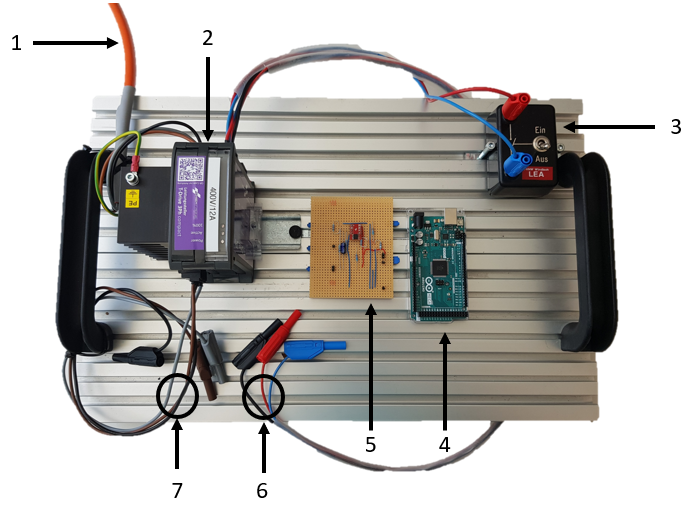
\includegraphics[width=\textwidth]{Aufbau_Messung.png}	
	\caption{Aufbau der Messung}\label{fig:Aufbau Messung}
\end{figure}
\todo{besserer Titel wählen}

\begin{table}[ht!]
	\centering
	\begin{tabular}{|l|l|}
		\hline
		Nummer & Bauteil                                       \\ \hline
		1      & Eingangskabel Thyristorsteller                \\ \hline
		2      & Thyristorsteller                              \\ \hline
		3      & Freigabe Thyristorsteller                     \\ \hline
		4      & Arduino Mega2560                              \\ \hline
		5      & Steckbrett mit Spannungsverstärkungsschaltung \\ \hline
		6      & Ansteuerung Thyristorsteller                  \\ \hline
		7      & Ausgang Thyristorsteller                      \\ \hline
	\end{tabular}
	\caption{Beschreibung der Nummern des Laboraufbaus}\label{tab:Nummern_Laboraufbau}
\end{table}





\newpage
\subsection{Messungen Ströme}
Die Ströme der verschiedenen Ansteuerungarten und Verbrauchern sind auf zu- und unzulässige Oberschwingungen zu untersuchen. Sie müssen zwingend die Werte der Normen \ref{sec:Normen} einhalten. Ist dies der Fall, werden anschliessend noch die Spannungen untersucht. Halten Ansteuerungsarten die Normen nicht ein, werden die Spannungen nicht behandelt. Bei den Schwingungspaketsteuerungen werden die Ströme nicht angeschaut, da die nicht von Interesse sind. Damit man jedoch einen Vergleich zur Simulation hat ist diese Ansteuerung bei der Spannung aufgelistet. Die Vergleiche werden immer mit Hilfe der FFT-Funktion von Matlab durchgeführt. 

\subsubsection{Messungen Widerstand}

Die Resultate der Strommessungen sind wie folgt aufgebaut: Bei den Abbildungen \ref{fig:Mess_Widerstand_Phas_60grad_stroeme}, \ref{fig:Mess_Widerstand_Phas_90grad_stroeme}, \ref{fig:Mess_Widerstand_Sanft_stroeme} und \ref{fig:Mess_Widerstand_Sanft_langsam_stroeme} sind zuerst die Ströme, die durch den Culatti fliessen dargestellt. Der Culatti ist ein ohmscher Widerstand mit dem Wert von \SI{150}{\Omega} pro Strang. Der maximale Effektivstrom, der dabei durchgelassen werden darf, ist \SI{2.4}{A}. Die zweite Grafik zeigt das FFT des gemessenen Stromes, jedoch nur von einer Phase an. Da sich alle drei Phasen gleich verhalten, werden die anderen zwei nicht angezeigt. Da die Grenzwerte der Oberschwingungsströme einen maximalen Wert von bis zu \SI{16}{A} Effektivwert behandelt, wurde der gemessene Wert auf die \SI{16}{A} hochgerechnet. Dies ist in der dritten Grafik der jeweiligen Abbildung ersichtlich. Anschliessend berechnete man von diesen Ströme das FFT und verglich die Werte der Amplitude tabellarisch mit den dazugehörigen Normen \ref{sec:Stromnormen}, ersichtlich in der Tabelle \ref{tab:Grenzwerte_Normen}.

\subsubsection*{Phasenanschnitt 60\textdegree}

In der Abbildung \ref{fig:Mess_Widerstand_Phas_60grad_stroeme} ist das Stromsignal mit einem Phasenanschnittswinkel von 60\textdegree \hspace{0.02cm} ersichtlich. 

\begin{figure}[ht!]
	\centering
	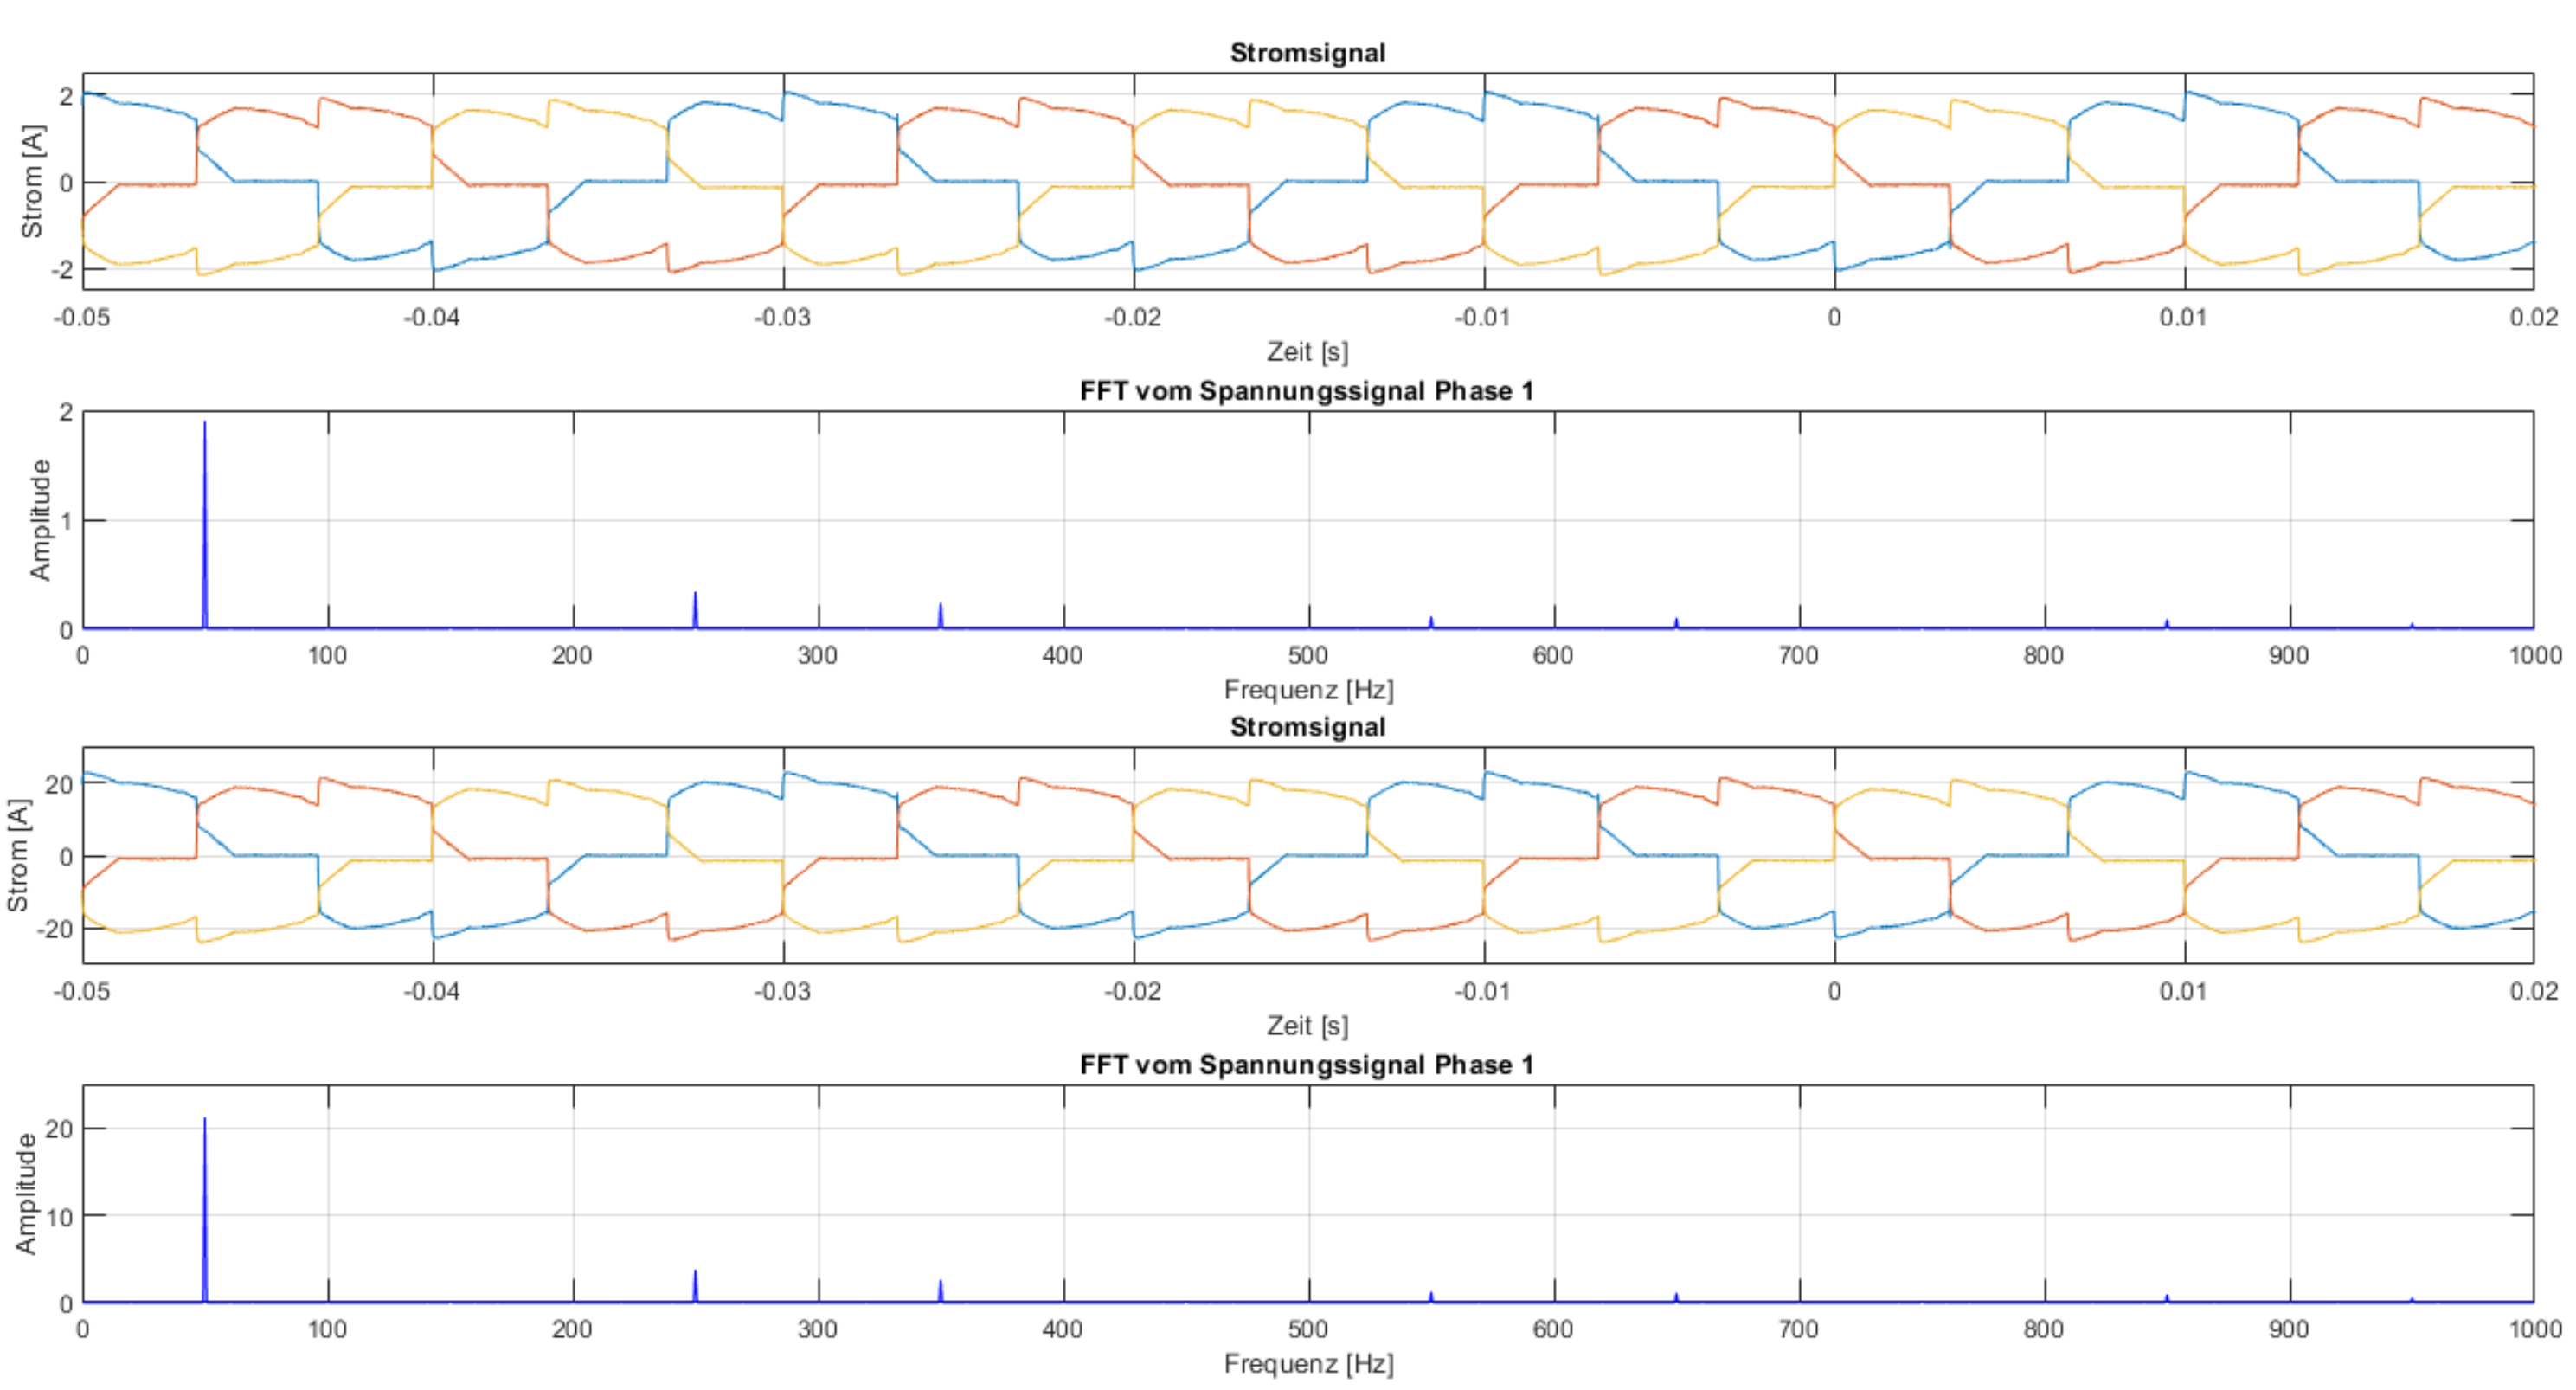
\includegraphics[width=\textwidth]{Messung_Widerstand_Phas_60grad_stroeme.png}	
	\caption{Messung mit Phasenanschnitt 60\textdegree}\label{fig:Mess_Widerstand_Phas_60grad_stroeme}
\end{figure}


\begin{table}[ht!]
	\centering
	\begin{tabular}{|l|l|l|}
		\hline
		Oberschwingungsordnung & Amplitude [A] 	& Verhältnis zur Grundschwingung	\\ \hline
		1                      & 21.1996   		& 100\%								\\ \hline
		5                      & 3.7851    		& 17.86\%							\\ \hline
		7                      & 2.6127    		& 12.32\%							\\ \hline
		11                     & 1.2267    		& 5.79\%							\\ \hline
	\end{tabular}
	\caption{Amplitudenwerte bei den harmonischen Oberschwingungen bei Phasenanschnitt 60\textdegree}\label{tab:Phas_60_Stroeme}
\end{table}
%Die Höhe der Amplituden der Oberschwingungen der Tabelle \ref{tab:Phas_60_Stroeme} können mit den Normen in der Tabelle \ref{tab:Grenzwerte_Normen} verglichen werden. Dabei wird festgestellt, dass die Werte der Messung höher sind als die Normen zulassen.

Wenn die Werten der Messungen in der Tabelle \ref{tab:Phas_60_Stroeme} mit den Werten der Normen in der Tabelle \ref{tab:Grenzwerte_Normen} verglichen werden, ist ersichtlich, dass die Amplitudenwerte bei der 5. bis 11. Oberschwingungsordnung zu hoch sind. Es kann gesagt werden, dass sich der Phasenanschnitt mit 60\textdegree \hspace{0.02cm} nicht eignet um den Widerstand anzusteuern, da dies nicht den Normen entspricht. Die Spannungen werden deshalb nicht mehr untersucht. 


\subsubsection*{Phasenanschnitt 90\textdegree}

Die Abbildung \ref{fig:Mess_Widerstand_Phas_90grad_stroeme} zeigt die Ansteuerung mit einem Phasenanschnitt von 90\textdegree \hspace{0.02cm}. 

\begin{figure}[ht!]
	\centering
	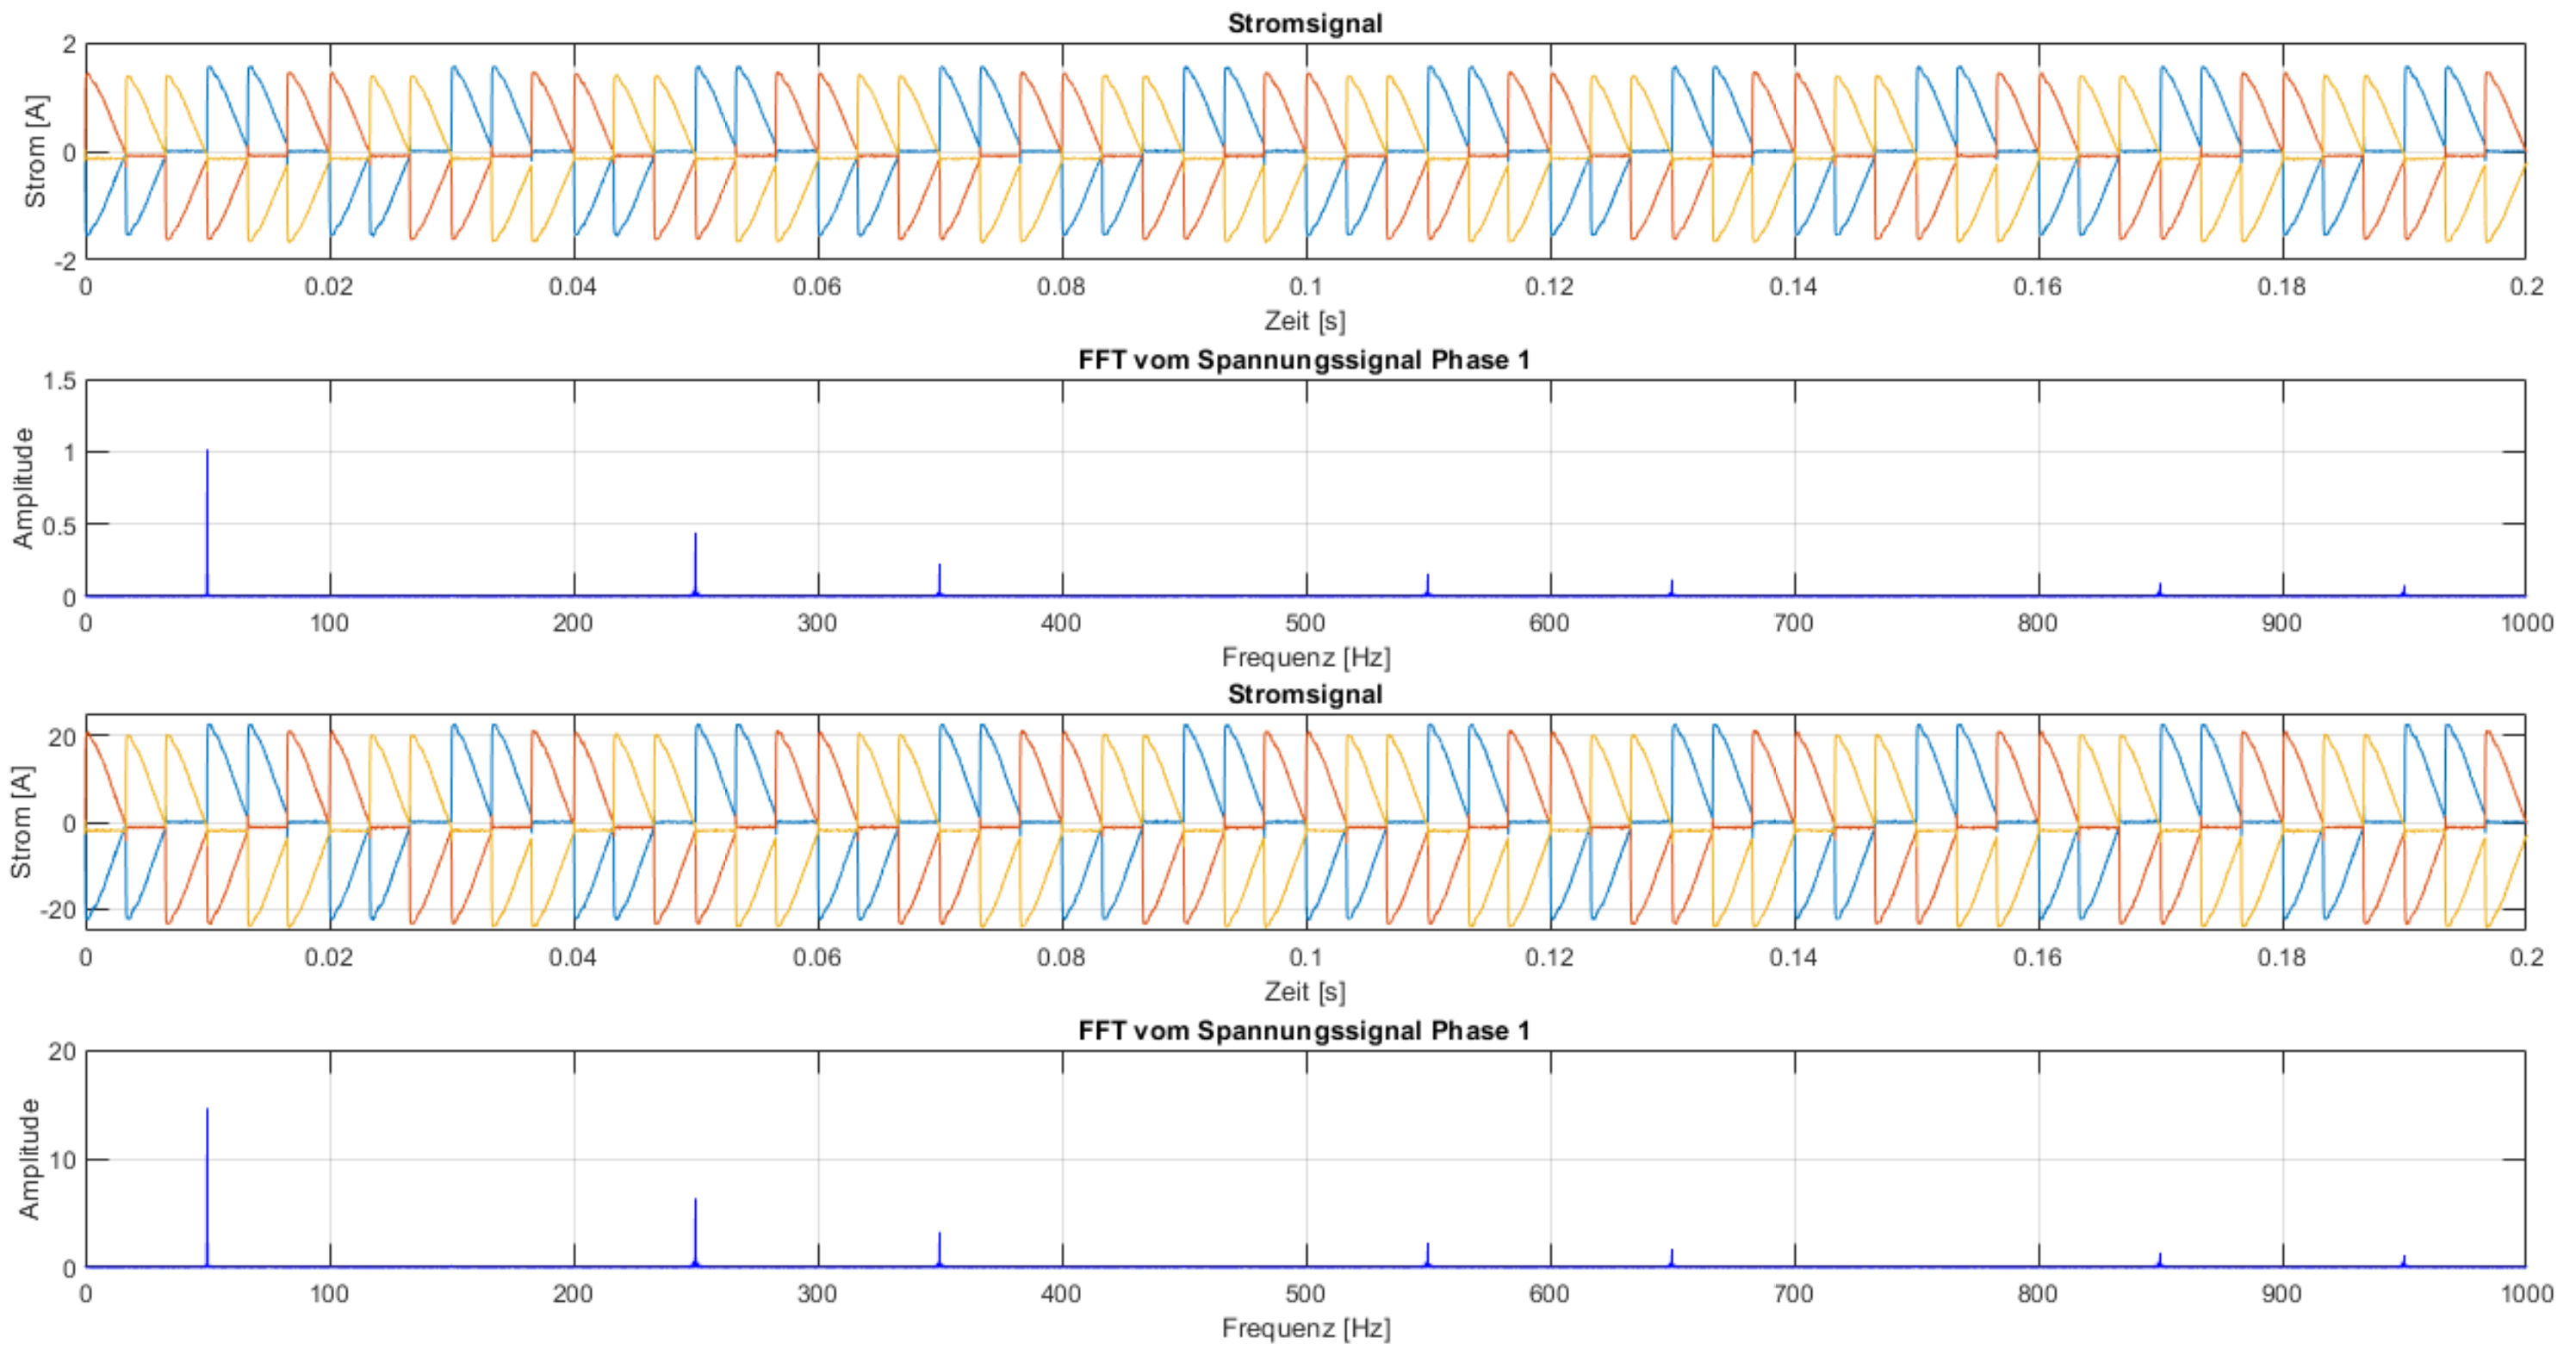
\includegraphics[width=\textwidth]{Messung_Widerstand_Phas_90grad_stroeme.png}	
	\caption{Phasenanschnitt 90\textdegree}\label{fig:Mess_Widerstand_Phas_90grad_stroeme}
\end{figure}

\begin{table}[ht!]
	\centering
	\begin{tabular}{|l|l|l|}
		\hline
		Oberschwingungsordnung 	& Amplitude [A] & Verhältnis zur Grundschwingung	\\ \hline
		1       				& 14.647   		& 100\%								\\ \hline
		5      					& 6.3481    	& 43.34\%							\\ \hline
		7      					& 3.2571    	& 22.24\%							\\ \hline
		11      				& 2.273    		& 15.52\%							\\ \hline
	\end{tabular}
	\caption{Amplitudenwerte bei den harmonischen Oberschwingungen bei Phasenanschnitt 90\textdegree}\label{tab:Phas_90_Stroeme}
\end{table}

Die Amplitudenwerte der 5. bis 11. Oberschwingungsanordnung, erkennbar in der Tabelle \ref{tab:Phas_90_Stroeme}, sind auch bei dieser Ansteuerung, im Vergleich zu den Normen \ref{tab:Grenzwerte_Normen}, zu hoch. Somit eignet sich auch der Phasenanschnitt mit 90\textdegree \hspace{0.02cm} nicht, um den Widerstand anzusteuern. Auf die Spannung wird ebenfalls hier nicht mehr eingegangen. 


\newpage
\subsubsection*{Hartes Auf- und Absteuern}

In der Abbildung \ref{fig:Mess_Widerstand_Sanft_stroeme} ist das harte Auf- und Absteuern des Widerstands erkennbar. 

\begin{figure}[ht!]
	\centering
	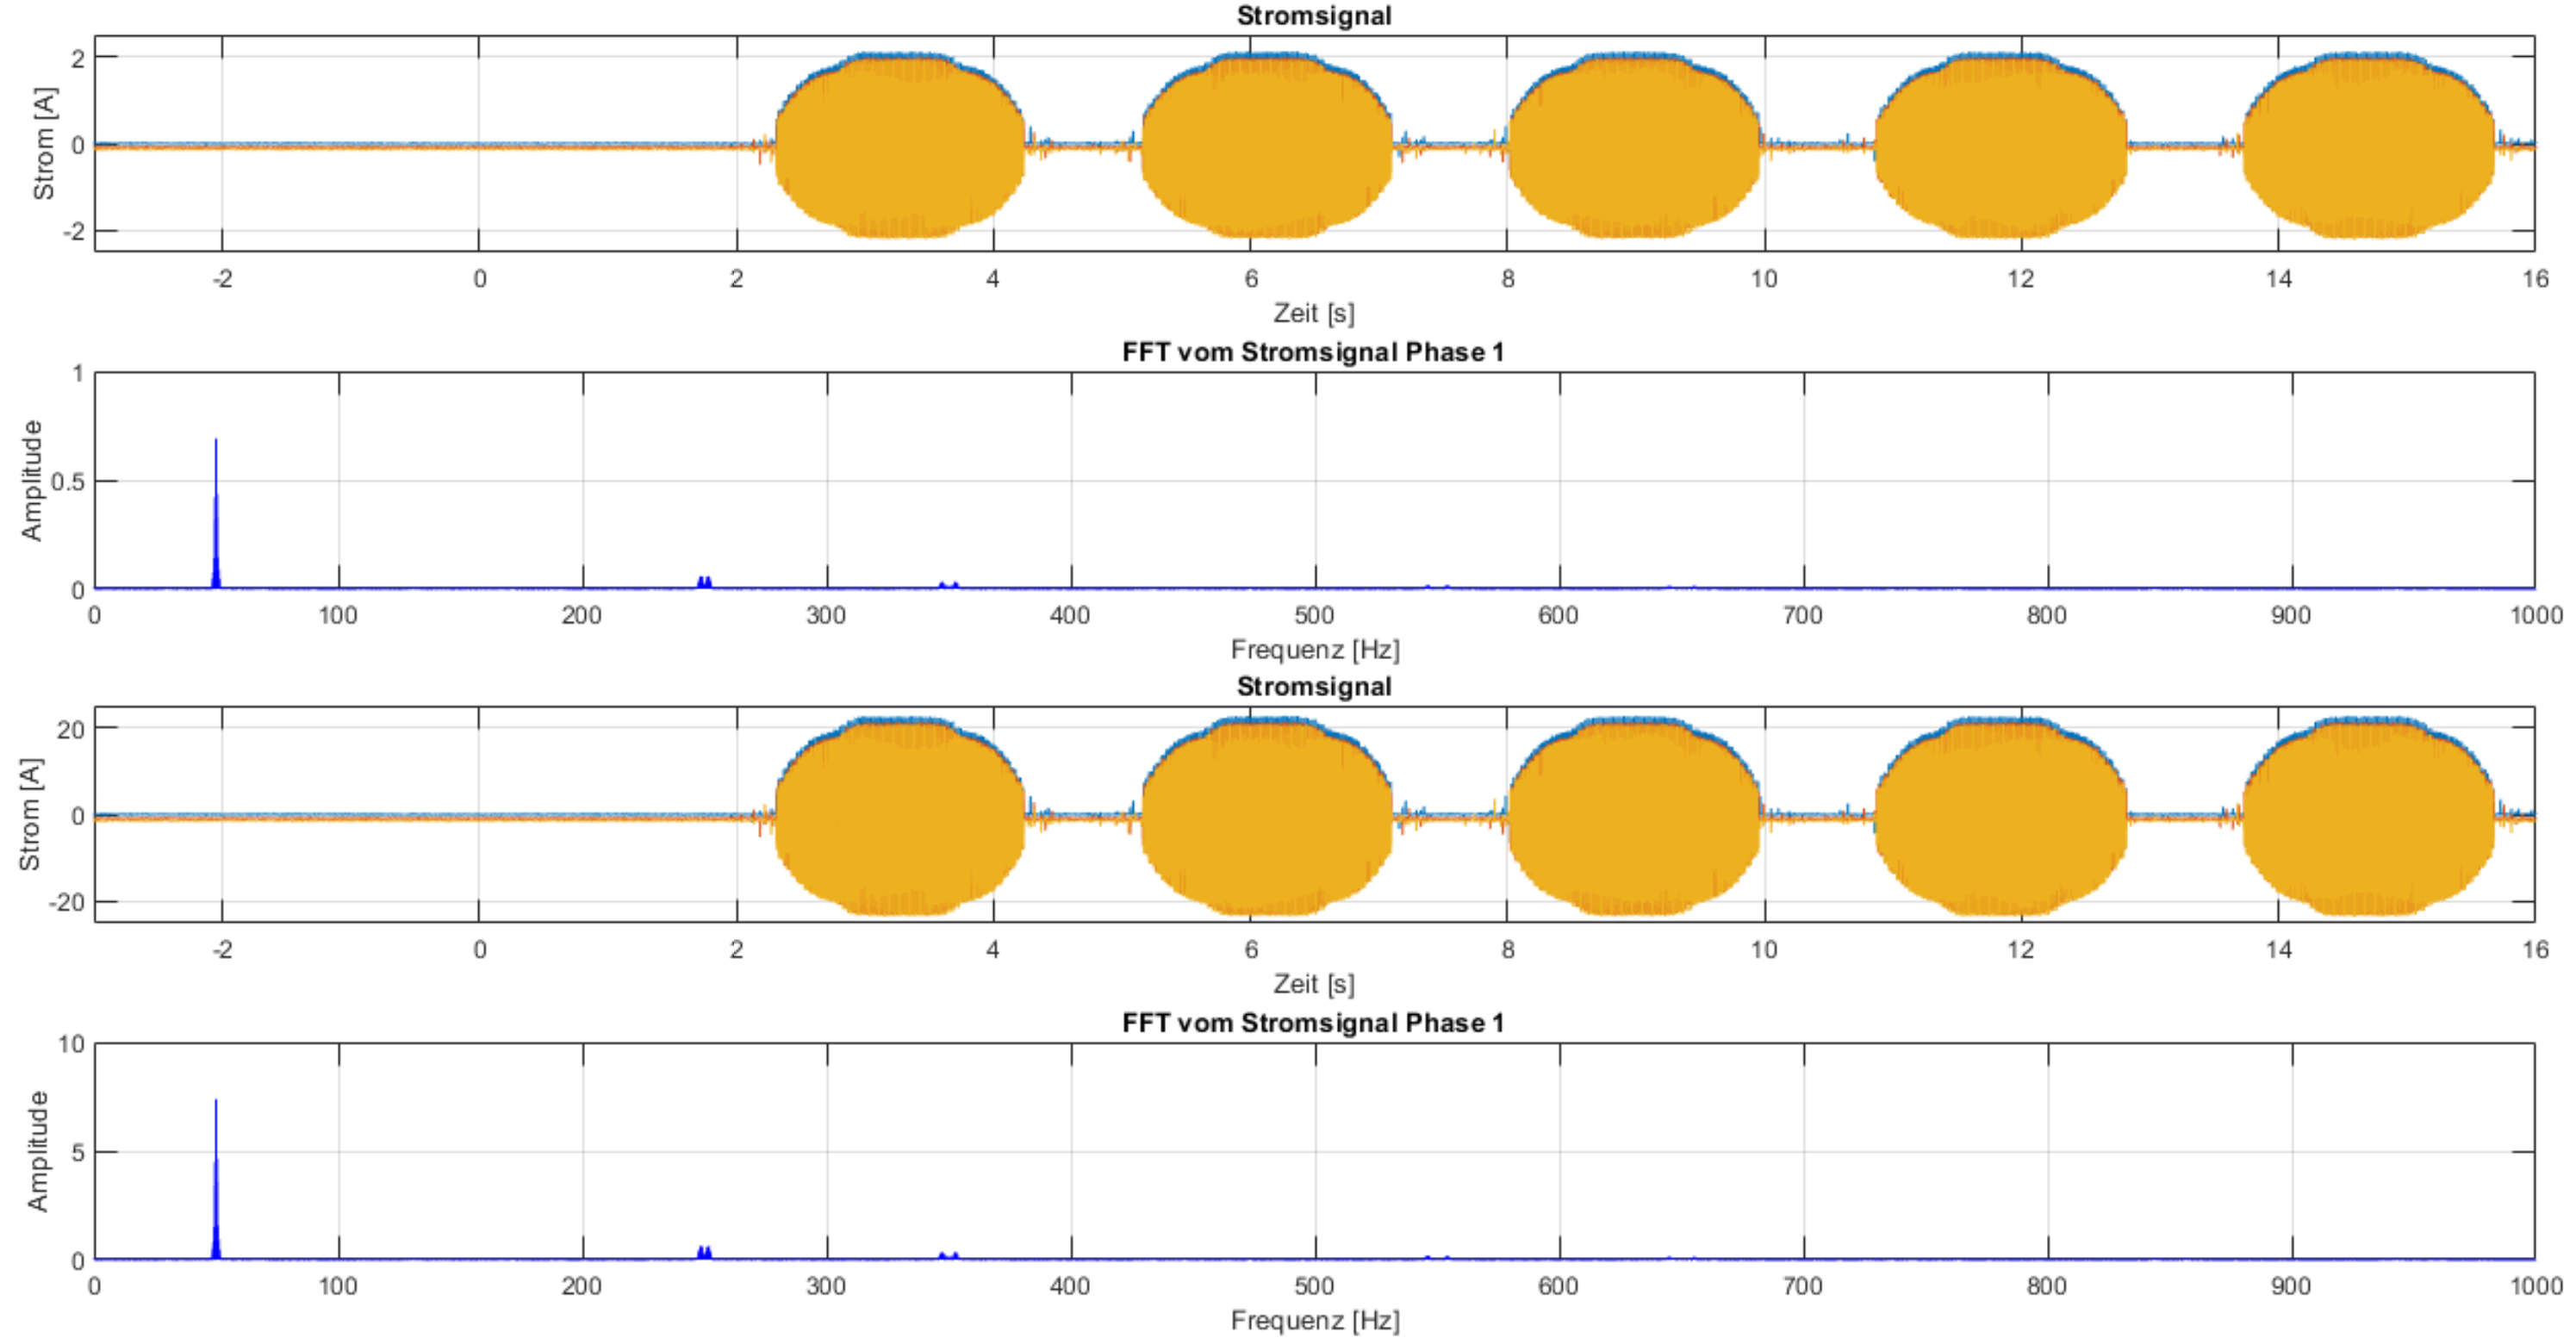
\includegraphics[width=\textwidth]{Messung_Widerstand_Sanft_stroeme.png}	
	\caption{Messung mit dem harten Auf- und Absteuern}\label{fig:Mess_Widerstand_Sanft_stroeme}
\end{figure}


\begin{table}[ht!]
	\centering
	\begin{tabular}{|l|l|l|}
		\hline
		Frequenz {[}Hz{]} & Amplitude {[}A{]} & Verhältnis zur Grundschwingung	\\ \hline
		49.3              & 1.5146            & 20.51\%							\\ \hline
		49.6              & 4.4853            & 60.73\%							\\ \hline
		49.7              & 2.618             & 35.45\%							\\ \hline
		50                & 7.3857            & 100\%							\\ \hline
		50.05             & 3.73              & 50.5\%							\\ \hline
		50.35             & 4.662             & 63.12\%							\\ \hline
		50.7              & 1.5504            & 21\%							\\ \hline
		248.65            & 0.6226            & 8.43\%							\\ \hline
		250               & 0.0883            & 1.2\%							\\ \hline
		251.45            & 0.6               & 8.12\%							\\ \hline
	\end{tabular}
	\caption{Amplitudenwerte bei verschiedenen Frequenzen beim hartem Auf- und Absteuern}\label{tab:Sanft_stroeme}
\end{table}
Da beim harten Auf- und Absteuern bereits die 5. harmonische Oberschwingung einen Amplitudenwert von  \SI{0.1}{A} hat, wurde darauf verzichtet weitere Werte der harmonischen Schwingungen tabellarisch aufzulisten. Jedoch sind bei dieser Messung die Sub- und Zwischenharmonische sehr interessant. Diese sind in der Tabelle \ref{tab:Sanft_stroeme} aufgeführt. Es ist ersichtlich, dass die Werte der Sub- und Zwischenharmonischen um \SI{50}{Hz}, mehr als die Hälfte der Grundschwingung, entsprechen. Diese sogenannten Seitenbänder sind auch bei den weiteren harmonischen Oberwellen erkennbar. Sie sind jedoch kleiner als die, um die \SI{50}{Hz}. Vergleicht man die Werte der Amplitude der Harmonischen sind sie im Bereich der erlaubten Grenzwerte. Deshalb wird noch eine Untersuchung der Spannung vorgenommen.


\newpage
\subsubsection*{Sanftes Auf- und Absteuern}\label{sec:Sanft_Widerstand_stroeme}
In Abbildung \ref{fig:Mess_Widerstand_Sanft_langsam_stroeme} erkennt man ein sanftes Auf- und Absteuern der Ströme.

\begin{figure}[ht!]
	\centering
	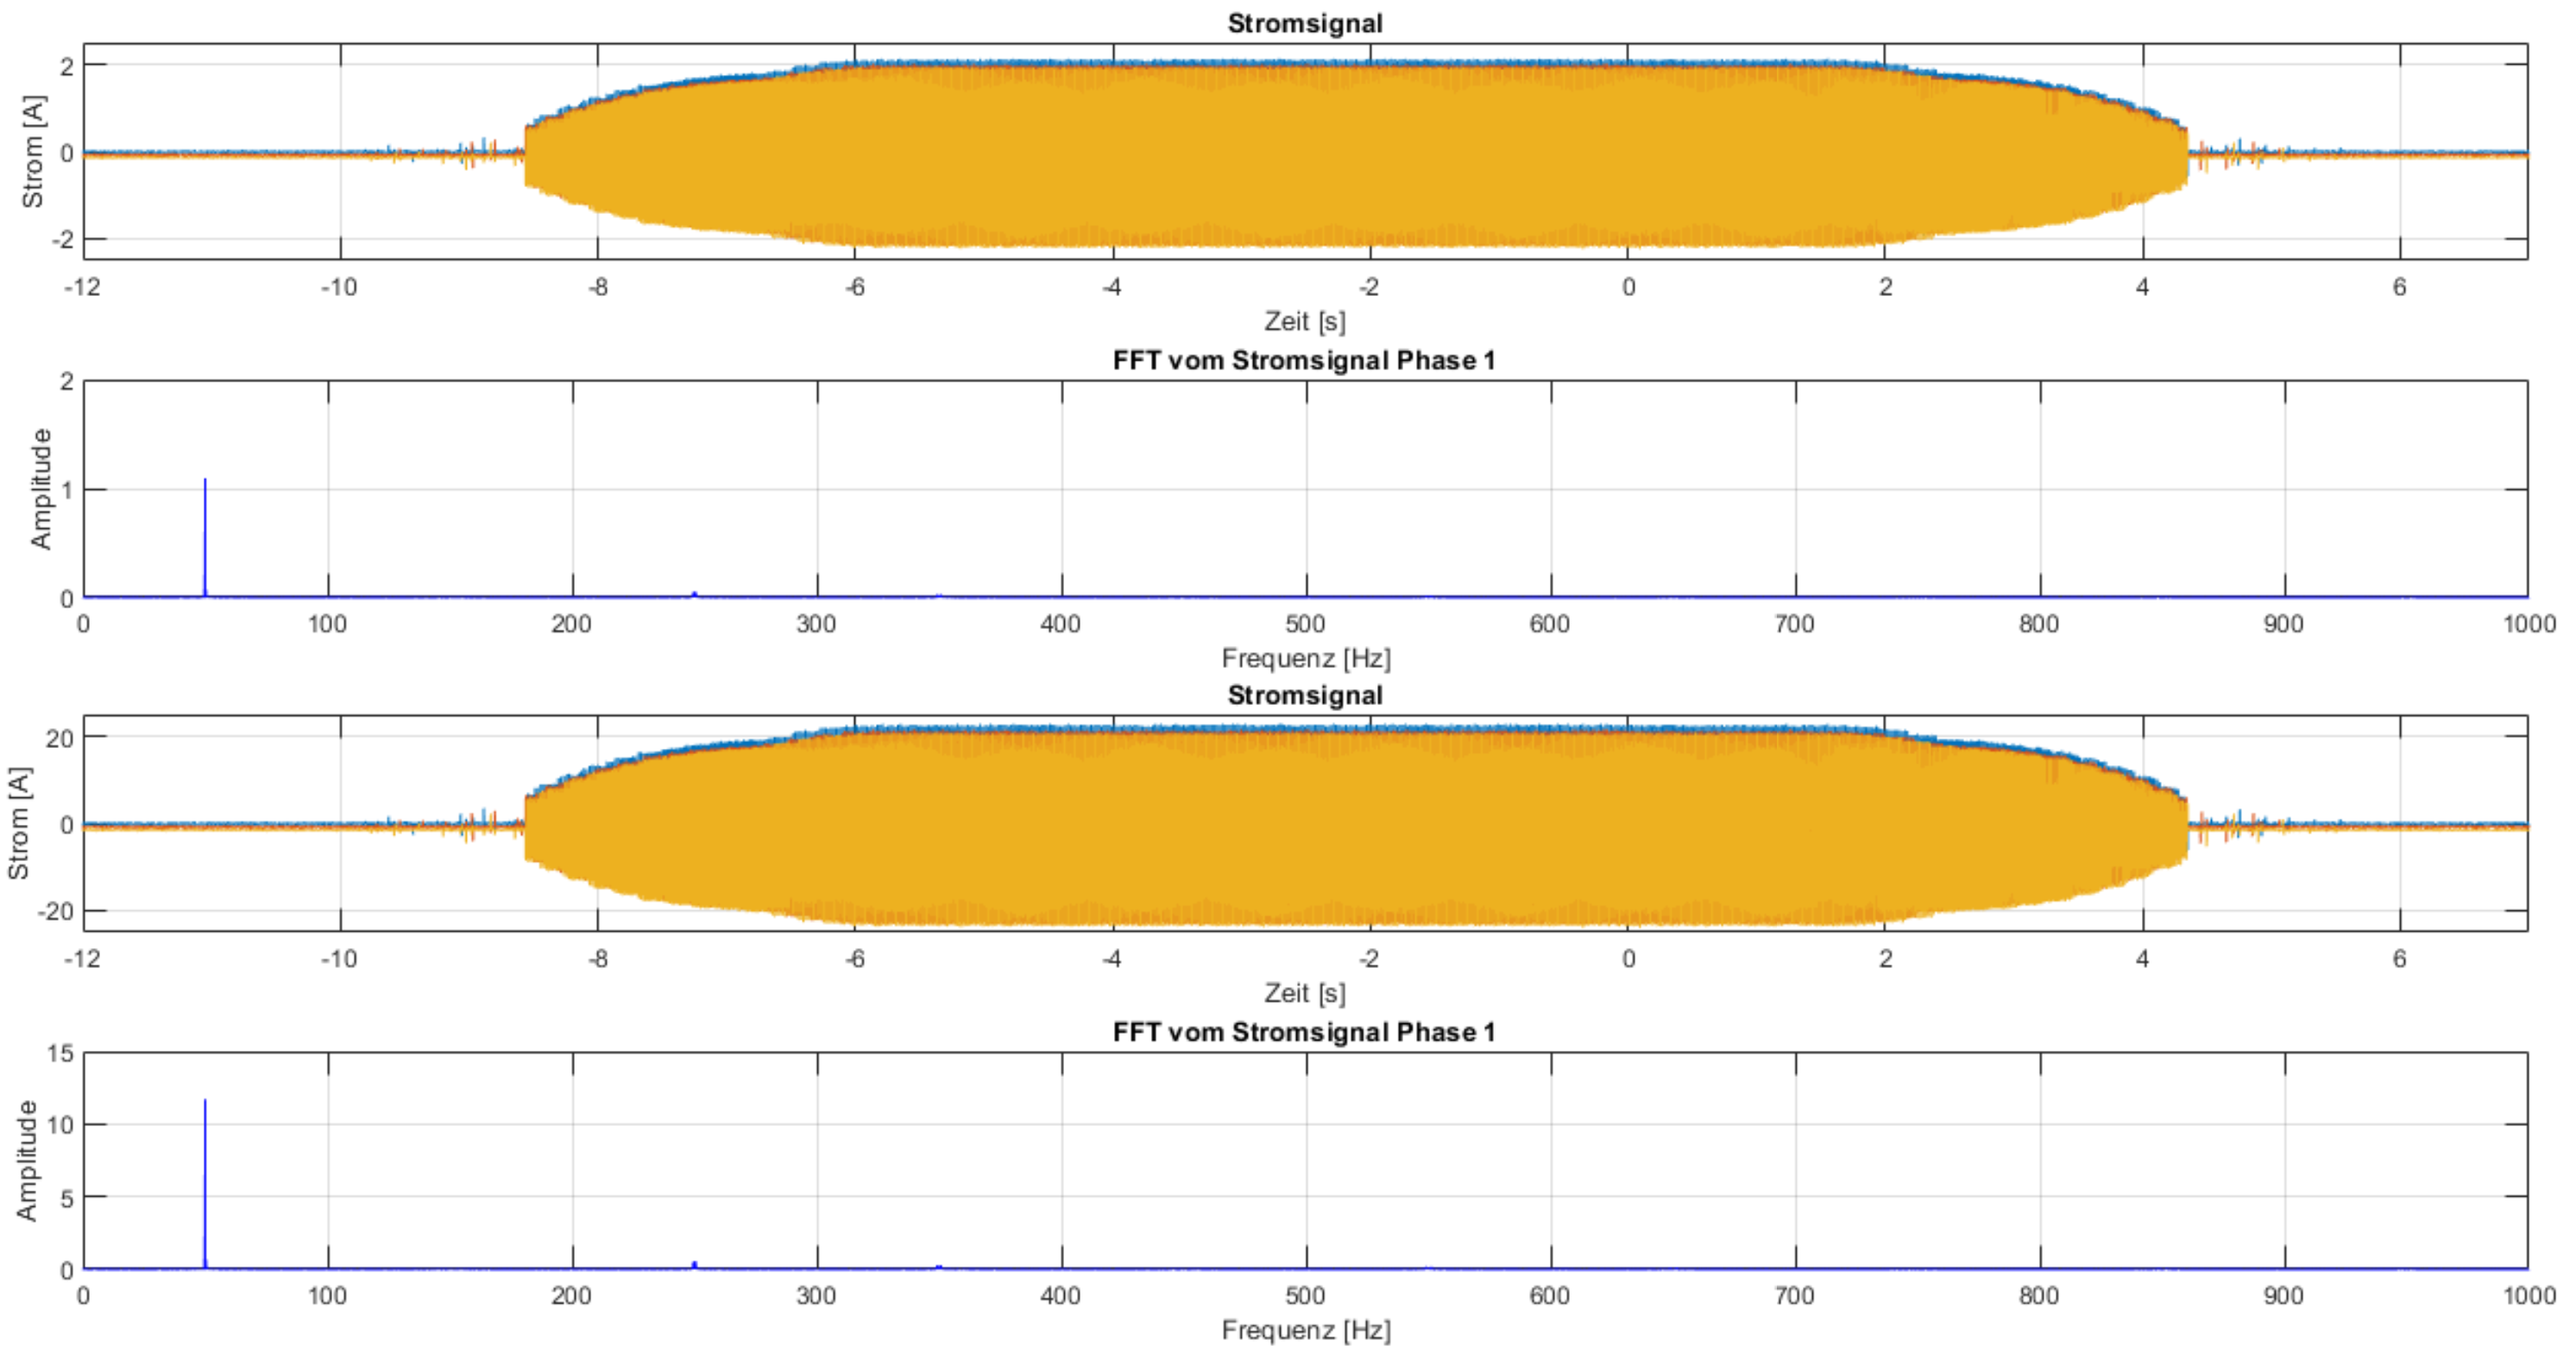
\includegraphics[width=\textwidth]{Messung_Widerstand_Sanft_langsam_stroeme.png}	
	\caption{Messung mit sanftem Auf- und Absteuern}\label{fig:Mess_Widerstand_Sanft_langsam_stroeme}
\end{figure}

\begin{table}[ht!]
	\centering
	\begin{tabular}{|l|l|l|}
		\hline
		Frequenz {[}Hz{]} & Amplitude {[}A{]} & Verhältnis zur Grundschwingung	\\ \hline
		49.8              & 1.148             & 9.8\%							\\ \hline
		49.85             & 1.786             & 15.25\%							\\ \hline
		49.9              & 1.519             & 12.97\%							\\ \hline
		49.95             & 6.703             & 57.22\%							\\ \hline
		50                & 11.715            & 100\%							\\ \hline
		50.05             & 7.136             & 60.91\%							\\ \hline
		50.1              & 1.473             & 12.57\%							\\ \hline
		50.15             & 1.923             & 16.41\%							\\ \hline
		249.65            & 0.563             & 4.81\%							\\ \hline
		250               & 0.186             & 1.59\%							\\ \hline
		250.35            & 0.559             & 4.77\%							\\ \hline
	\end{tabular}
	\caption{Amplitudenwerte bei den harmonischen Oberschwingungen beim sanftem Auf- und Absteuern}\label{tab:Sanft_langsam_stroeme}
\end{table}
Es ist zu erkennen, dass auch hier fast keine harmonische Oberwellen vorhanden sind. Die Amplitude der Grundschwingung ist jedoch höher als beim harten Auf- und Absteuern. Dies hat den Grund, dass länger auf der vollen Leistung gefahren wurde. Beim sanften Auf- und Absteuern ist das Hoch- und Runtergefahren langsamer, deshalb ist das Seitenband bei \SI{50}{Hz} kleiner. Dies erkennt man auch schon beim visuellen Vergleich der beiden Abbildungen \ref{fig:Mess_Widerstand_Sanft_langsam_stroeme} und \ref{fig:Mess_Widerstand_Sanft_stroeme}. Im Vergleich zum harten Auf- und Absteuern, ist die 5. Harmonische 0.39\% grösser, welches einem sehr kleinen Unterschied entspricht. Jedoch sind die Peaks der Seitenbänder näher bei \SI{50}{Hz}. Die Peaks des Seitenbandes bei \SI{250}{Hz} sind bei dem sanften Auf- und Absteuern kleiner als die beim harten Auf- und Absteuern.



\newpage
\subsubsection{Messungen Asynchronmaschine}
Um zu analysieren, wie sich das Signal bei einer ohmsch-induktiver Last verhält, wurden die Messungen mit einem Asynchronmotor wiederholt. Die Strommessung der ASM wurde mit den bekannten Phasenanschnittswinkeln und mit dem sanften Auf- und Absteuern vorgenommen. Dies hat den Grund, dass keine Anwendungen für das harte Auf- und Absteuern oder der Schwingungspaketsteuerung vorhanden sind. Ausserdem wird in der Praxis meistens der Phasenanschnitt verwendet. Wie auch schon beim Widerstand muss der Strom bei der ASM auf die \SI{16}{A} hochgerechnet werden, um diese mit den Norm tabellarisch vergleichen zu können. Die Messungen der Asynchronmaschine sind ähnlich aufgebaut wie die des Widerstands. Einzig das Spannungssignal des Drehzahlgebers wurde hinzugefügt. Es ist erkennbar, dass das jeweilige Hochfahren des Stromes einen Einfluss auf das Spannungssignal des Drehgeber hat. Je harter man hochfährt desto steiler wird die Kurve des Spannungssignal des Drehgeber. 


\subsubsection*{Phasenaschnitt 60\textdegree}
In Abbildung \ref{fig:Mess_Phas_60grad_stroeme} erkennt man ein einen Phasenanschnitt von 60\textdegree der Ströme.

\begin{figure}[ht!]
	\centering
	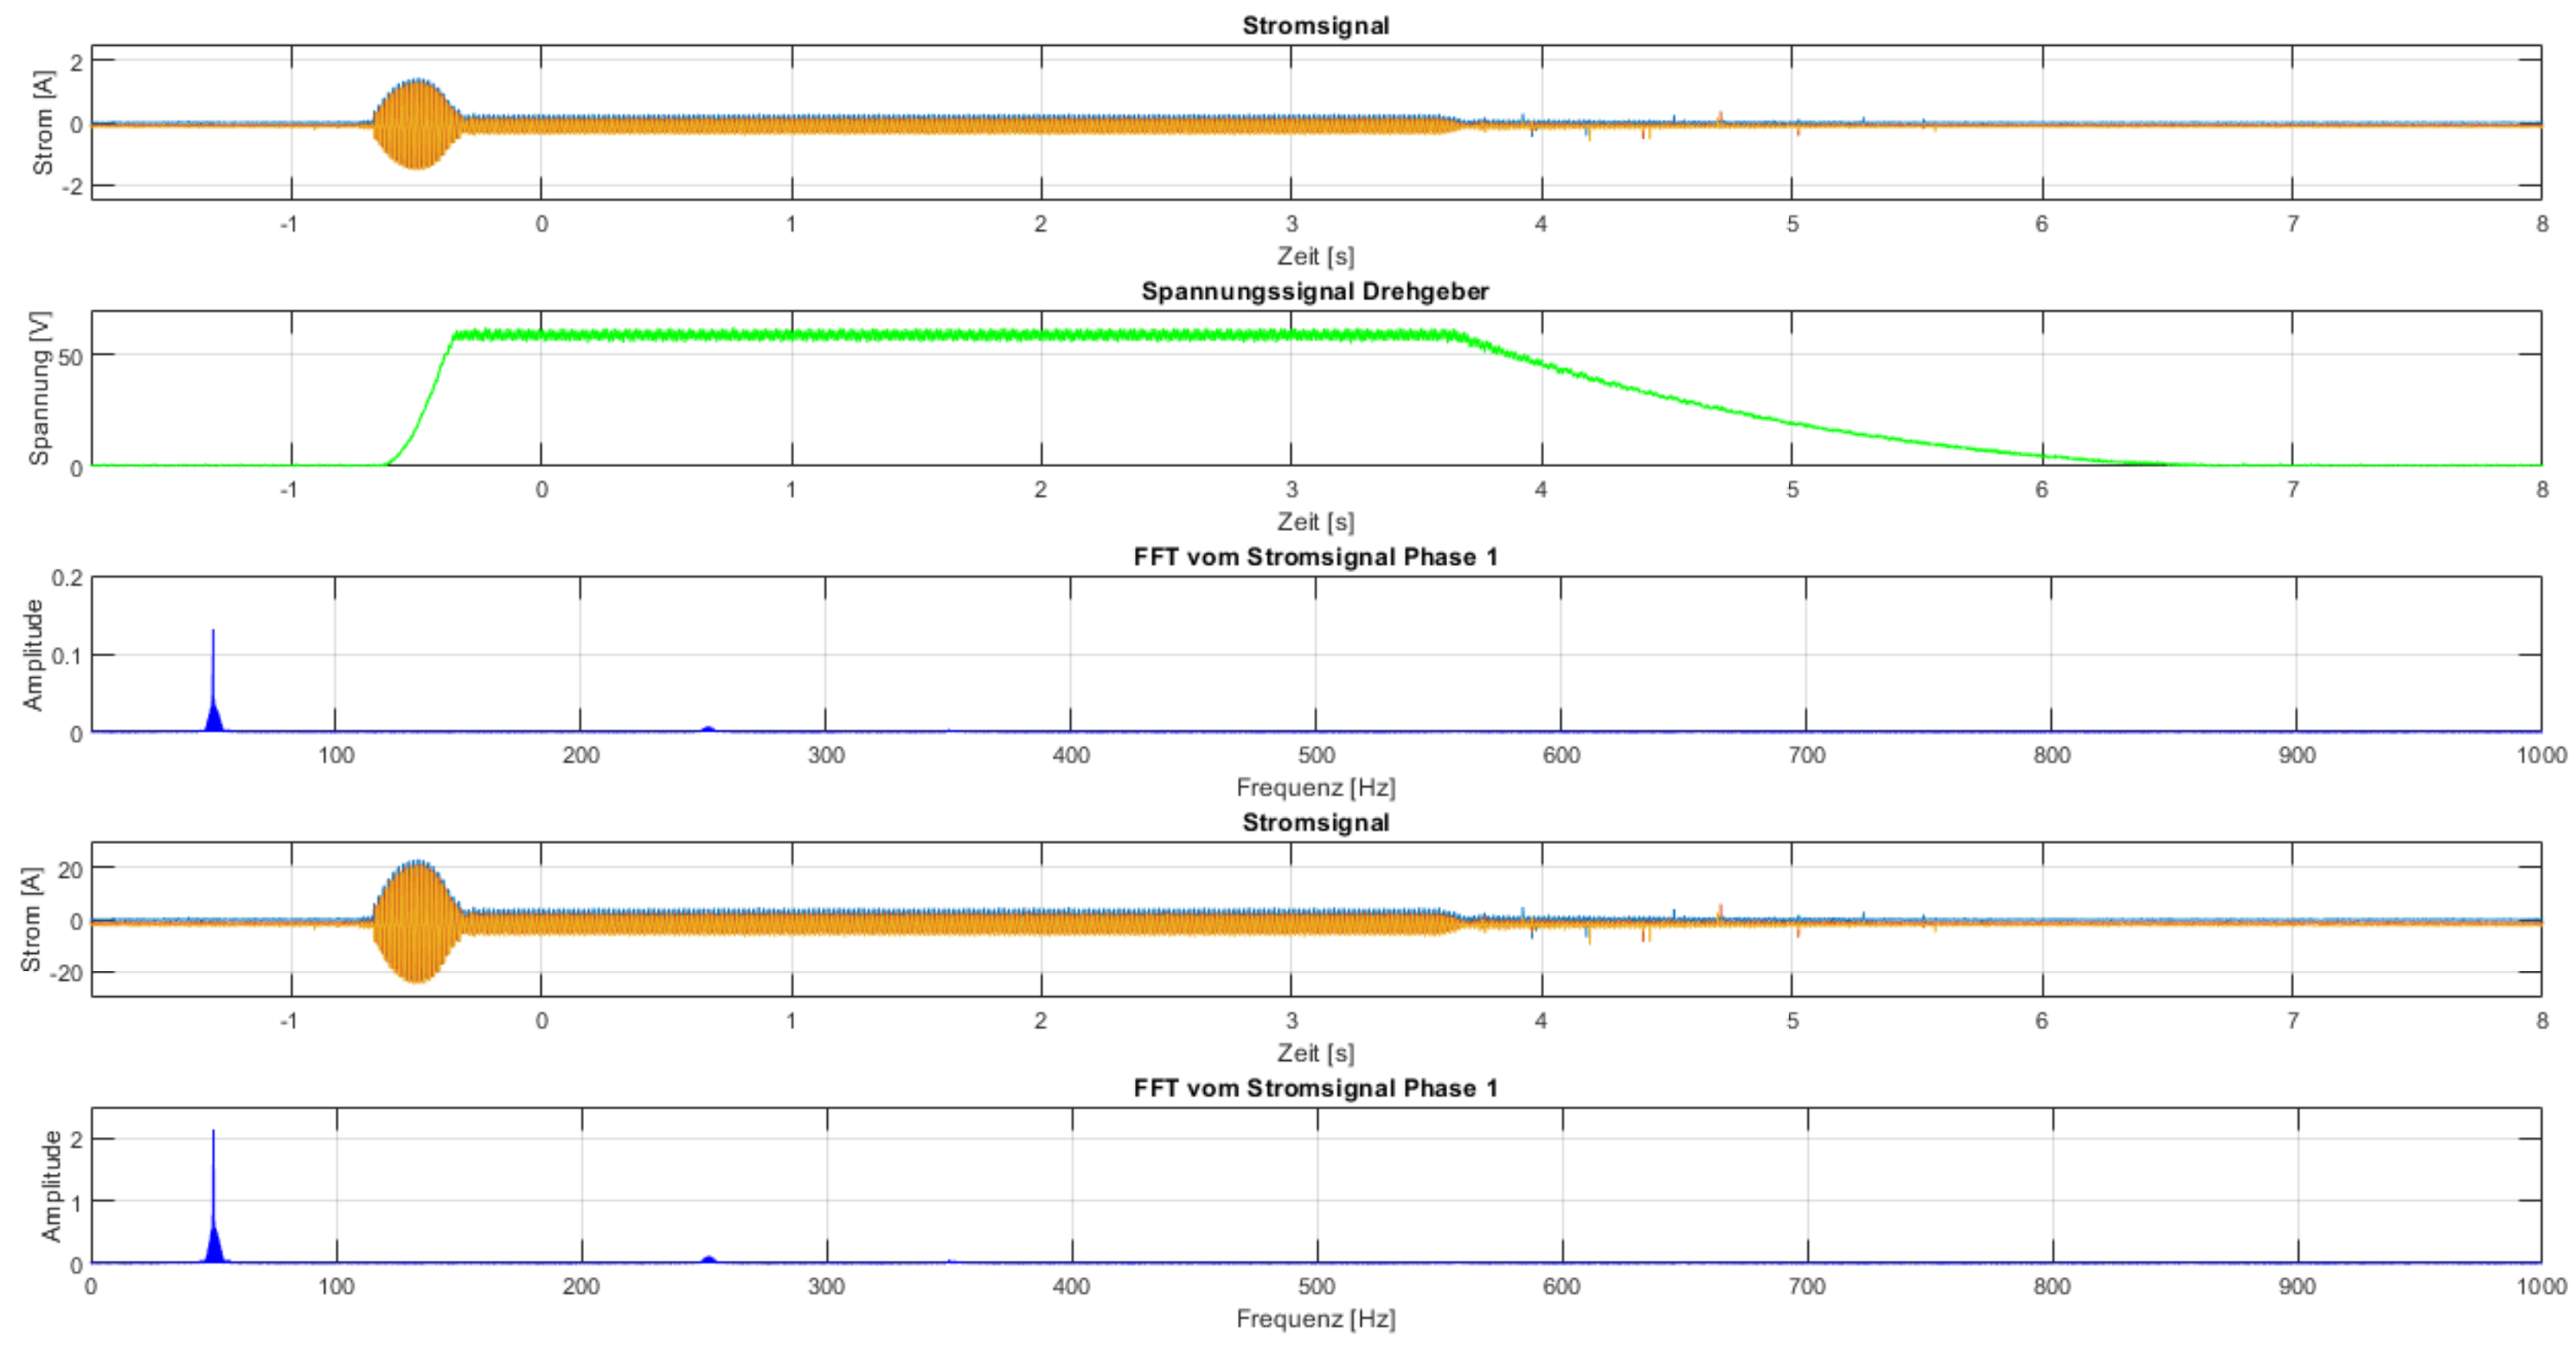
\includegraphics[width=\textwidth]{Messung_ASM_Phas_60grad_stroeme.png}	
	\caption{Messung mit Phasenanschnitt 60\textdegree}\label{fig:Mess_Phas_60grad_stroeme}
\end{figure}

\begin{table}[ht!]
	\centering
	\begin{tabular}{|l|l|l|}
		\hline
		Frequenz {[}Hz{]} & Amplitude {[}A{]} & Verhältnis zur Grundschwingung	\\ \hline
		49.7              & 0.76              & 35.53\%							\\ \hline
		49.9              & 1.317             & 61.57\%							\\ \hline
		50                & 2.139             & 100\%							\\ \hline
		50.1              & 1.53              & 71.53\%							\\ \hline
		50.3              & 0.675             & 31.56\%							\\ \hline
		250               & 0.07              & 3.27\%							\\ \hline
	\end{tabular}
	\caption{Amplitudenwerte bei den harmonischen Oberschwingungen bei Phasenanschnitt 60\textdegree}\label{tab:Phas_60_ASM_stroeme}
\end{table}
Entgegen den Vorkenntnissen bei Phasenanschnitt mit einem Winkel von 60\textdegree, gibt es bei der Ansteuerung der ASM praktisch keine harmonischen Oberwellen sondern fast nur Sub- und Zwischenharmonische. Dies hat den Grund, dass ein reiner Sinus von einer Frequenz von \SI{50}{Hz} bei der maximalen Drehzahl entsteht. Die fünfte harmonische Schwingung hat eine Amplitude von \SI{0.07}{A} und hält somit die Normen \ref{sec:Stromnormen} ein. Weitere Harmonische sind nicht zu erkennen. Die Peaks des Seitenbandes um die Grundschwingung sind im Verhältnis mit bis zu 70\% sehr hoch.


\subsubsection*{Phasenaschnitt 90\textdegree}

In Abbildung \ref{fig:Mess_Phas_90grad_stroeme} erkennt man einen Phasenanschnitt von 90\textdegree \hspace{0.02cm} der Ströme.

\begin{figure}[ht!]
	\centering
	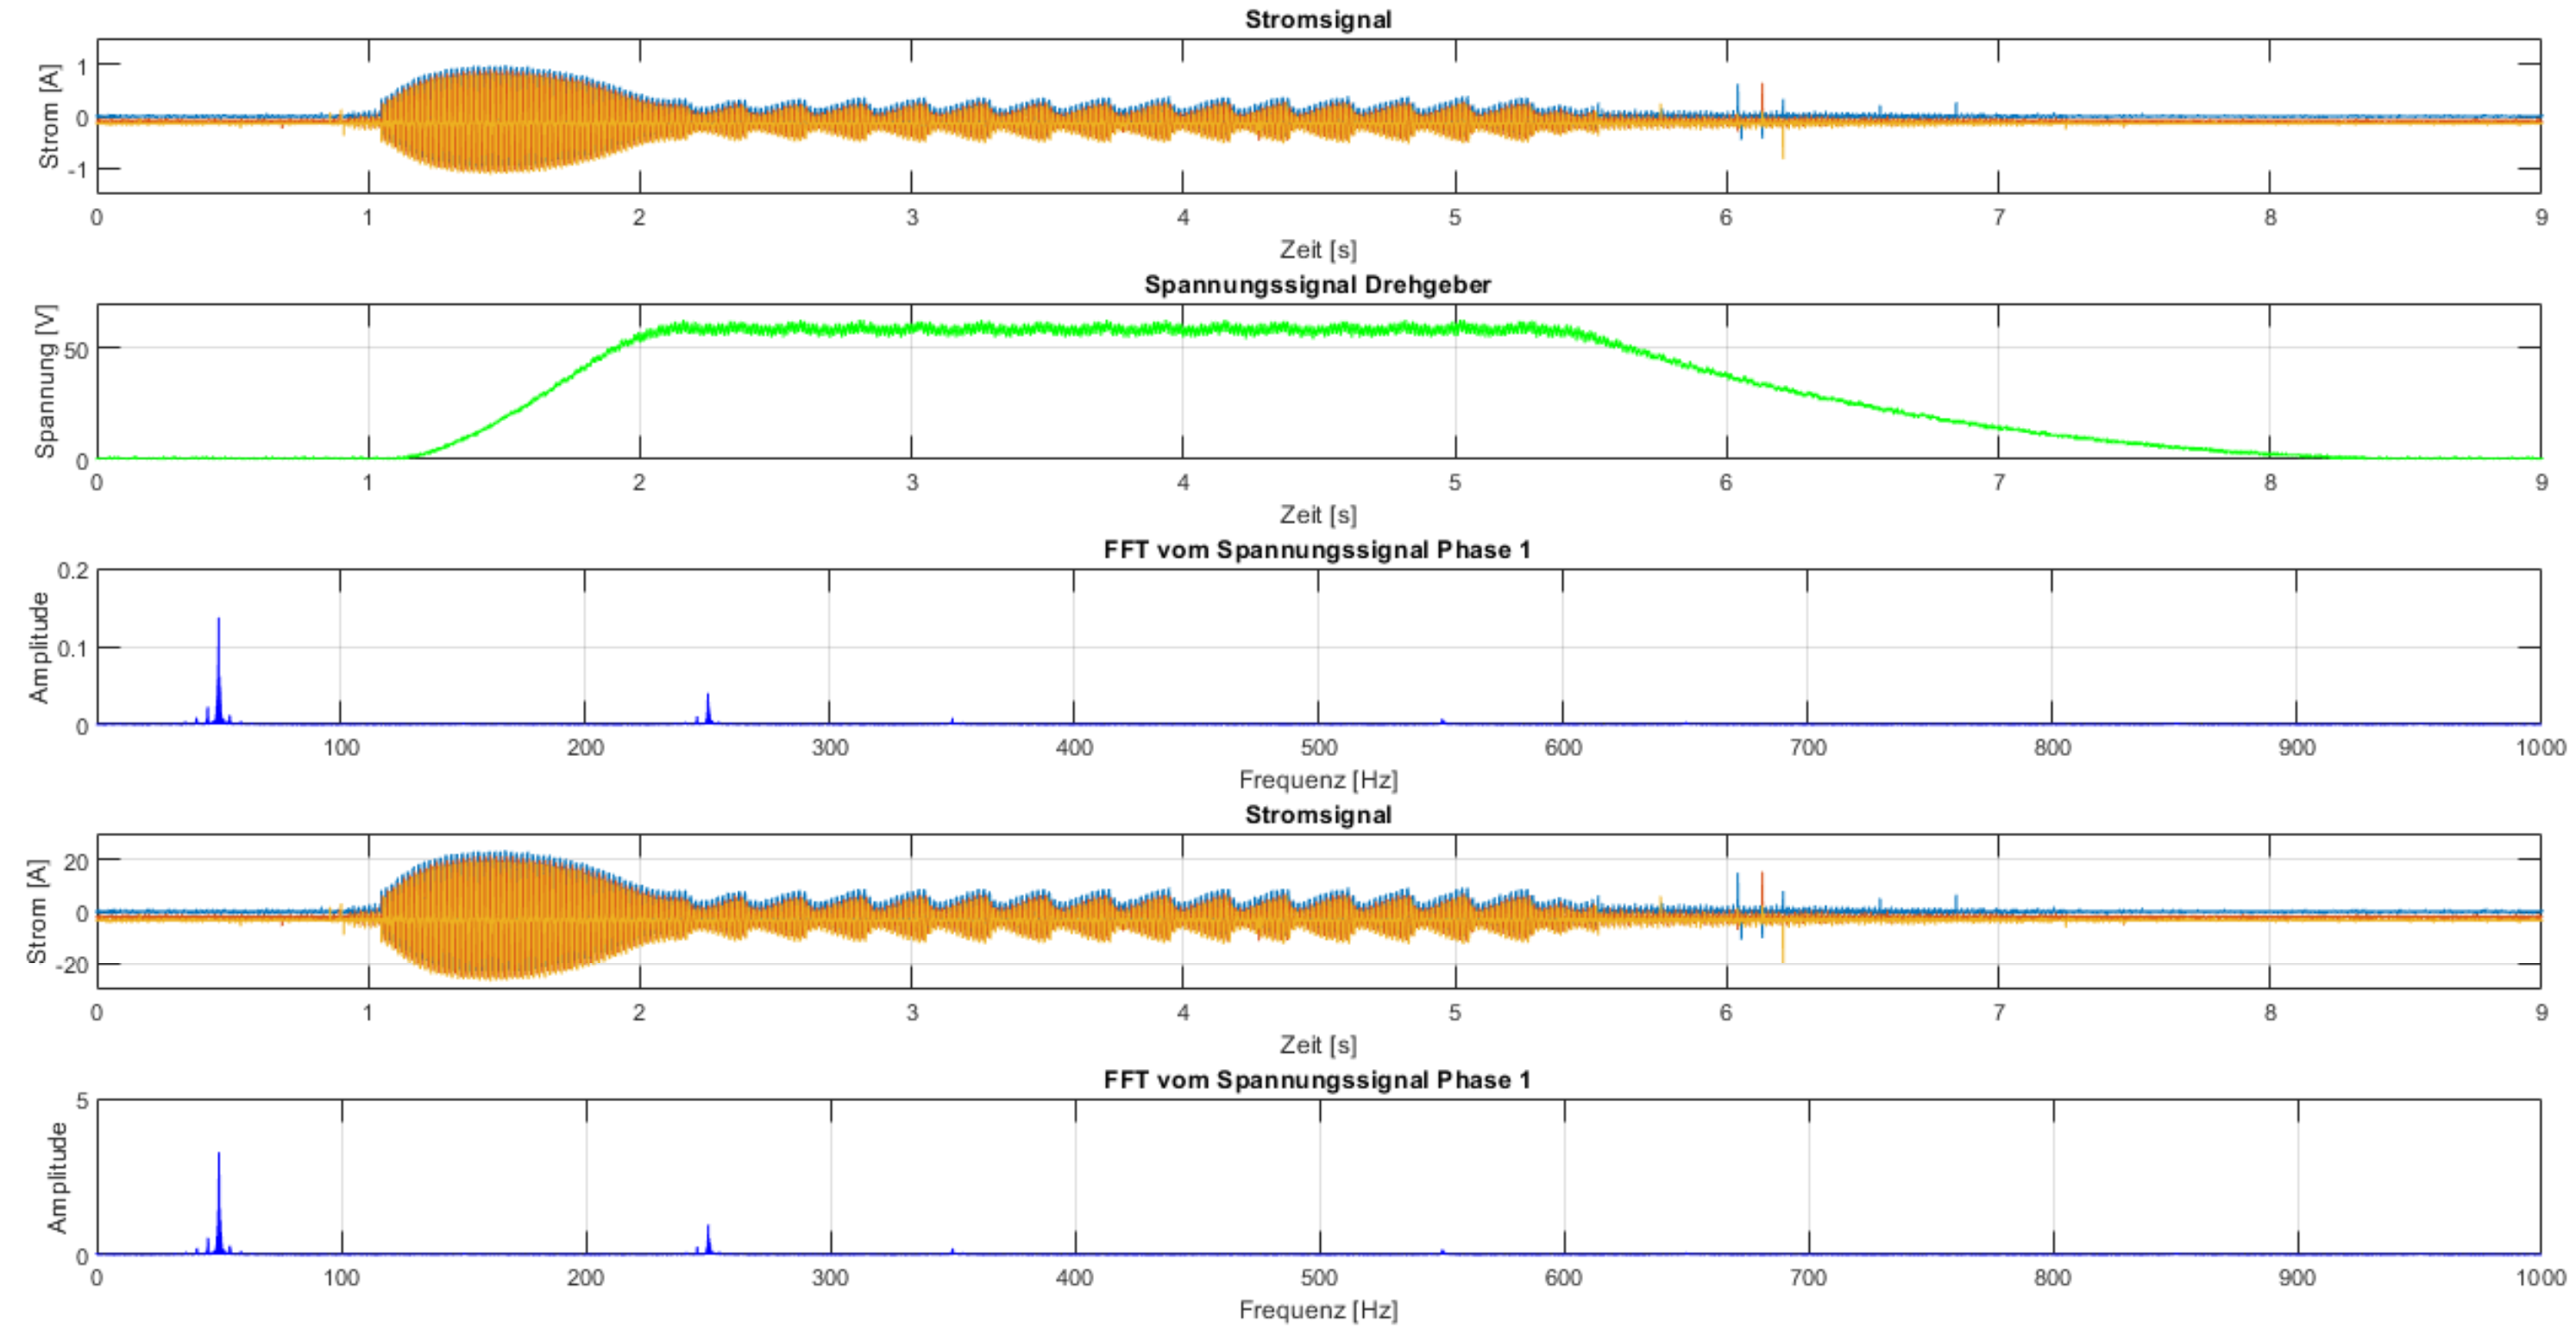
\includegraphics[width=\textwidth]{Messung_ASM_Phas_90grad_stroeme}	
	\caption{Messung mit Phasenanschnitt 90\textdegree}\label{fig:Mess_Phas_90grad_stroeme}
\end{figure}


\begin{table}[ht!]
	\centering
	\begin{tabular}{|l|l|l|}
		\hline
		Frequenz {[}Hz{]} & Amplitude {[}A{]} & Verhältnis zur Grundschwingung	\\ \hline
		49.7              & 1.399             & 42.6\%							\\ \hline
		49.9              & 2.023             & 61.61\%							\\ \hline
		50                & 3.2839            & 100\%							\\ \hline
		50.1              & 2.567             & 78.17\%							\\ \hline
		50.3              & 1.468             & 44.71\%							\\ \hline
		250               & 0.673             & 20.5\%							\\ \hline
		250.1             & 0.959             & 29.2\%							\\ \hline
		250.2             & 0.687             & 20.92\%							\\ \hline
	\end{tabular}
	\caption{Amplitudenwerte bei den harmonischen Oberschwingungen bei Phasenanschnitt 90\textdegree}\label{tab:Phas_90_ASM_stroeme}
\end{table}

Anders als bei der Ansteuerung mit dem Phasennaschnitt von 60\textdegree, treten mit 90\textdegree \hspace{0.02cm} bei der fünften Harmonischen grössere harmonische Oberwellen auf. Zusätzlich sind auch die Sub- und Zwischenharmonischen grösser als bei 60\textdegree. Auf der Abbildung \ref{fig:Mess_Phas_90grad_stroeme} ist beim Stromsignal ersichtlich, dass die Maschine schwingt. Dies wurde auch beim Testen festgestellt, dass die ASM nicht konstant auf der gleichen Drehzahl drehte. So kann diese Ansteuerungsart nicht verwendet werden um die Maschine anzusteuern. 
Im Vergleich zum Phasenanschnitt mit 60\textdegree sind die Peaks des Seitenbandes um die Grundschwingung noch höher. Auch die fünfte Harmonische entspricht im Verhältnis zur Grundschwingung 20.5\%. Die Amplitude jedoch ist immer noch kleiner als der erlaubte Grenzwert der Norm \ref{sec:Stromnormen}. 



\subsubsection*{Sanftes Auf- und Absteuern}

In Abbildung \ref{fig:Mess_Sanft_langsam_stroeme} erkennt man ein sanftes Auf- und Absteuern der Ströme.

\begin{figure}[ht!]
	\centering
	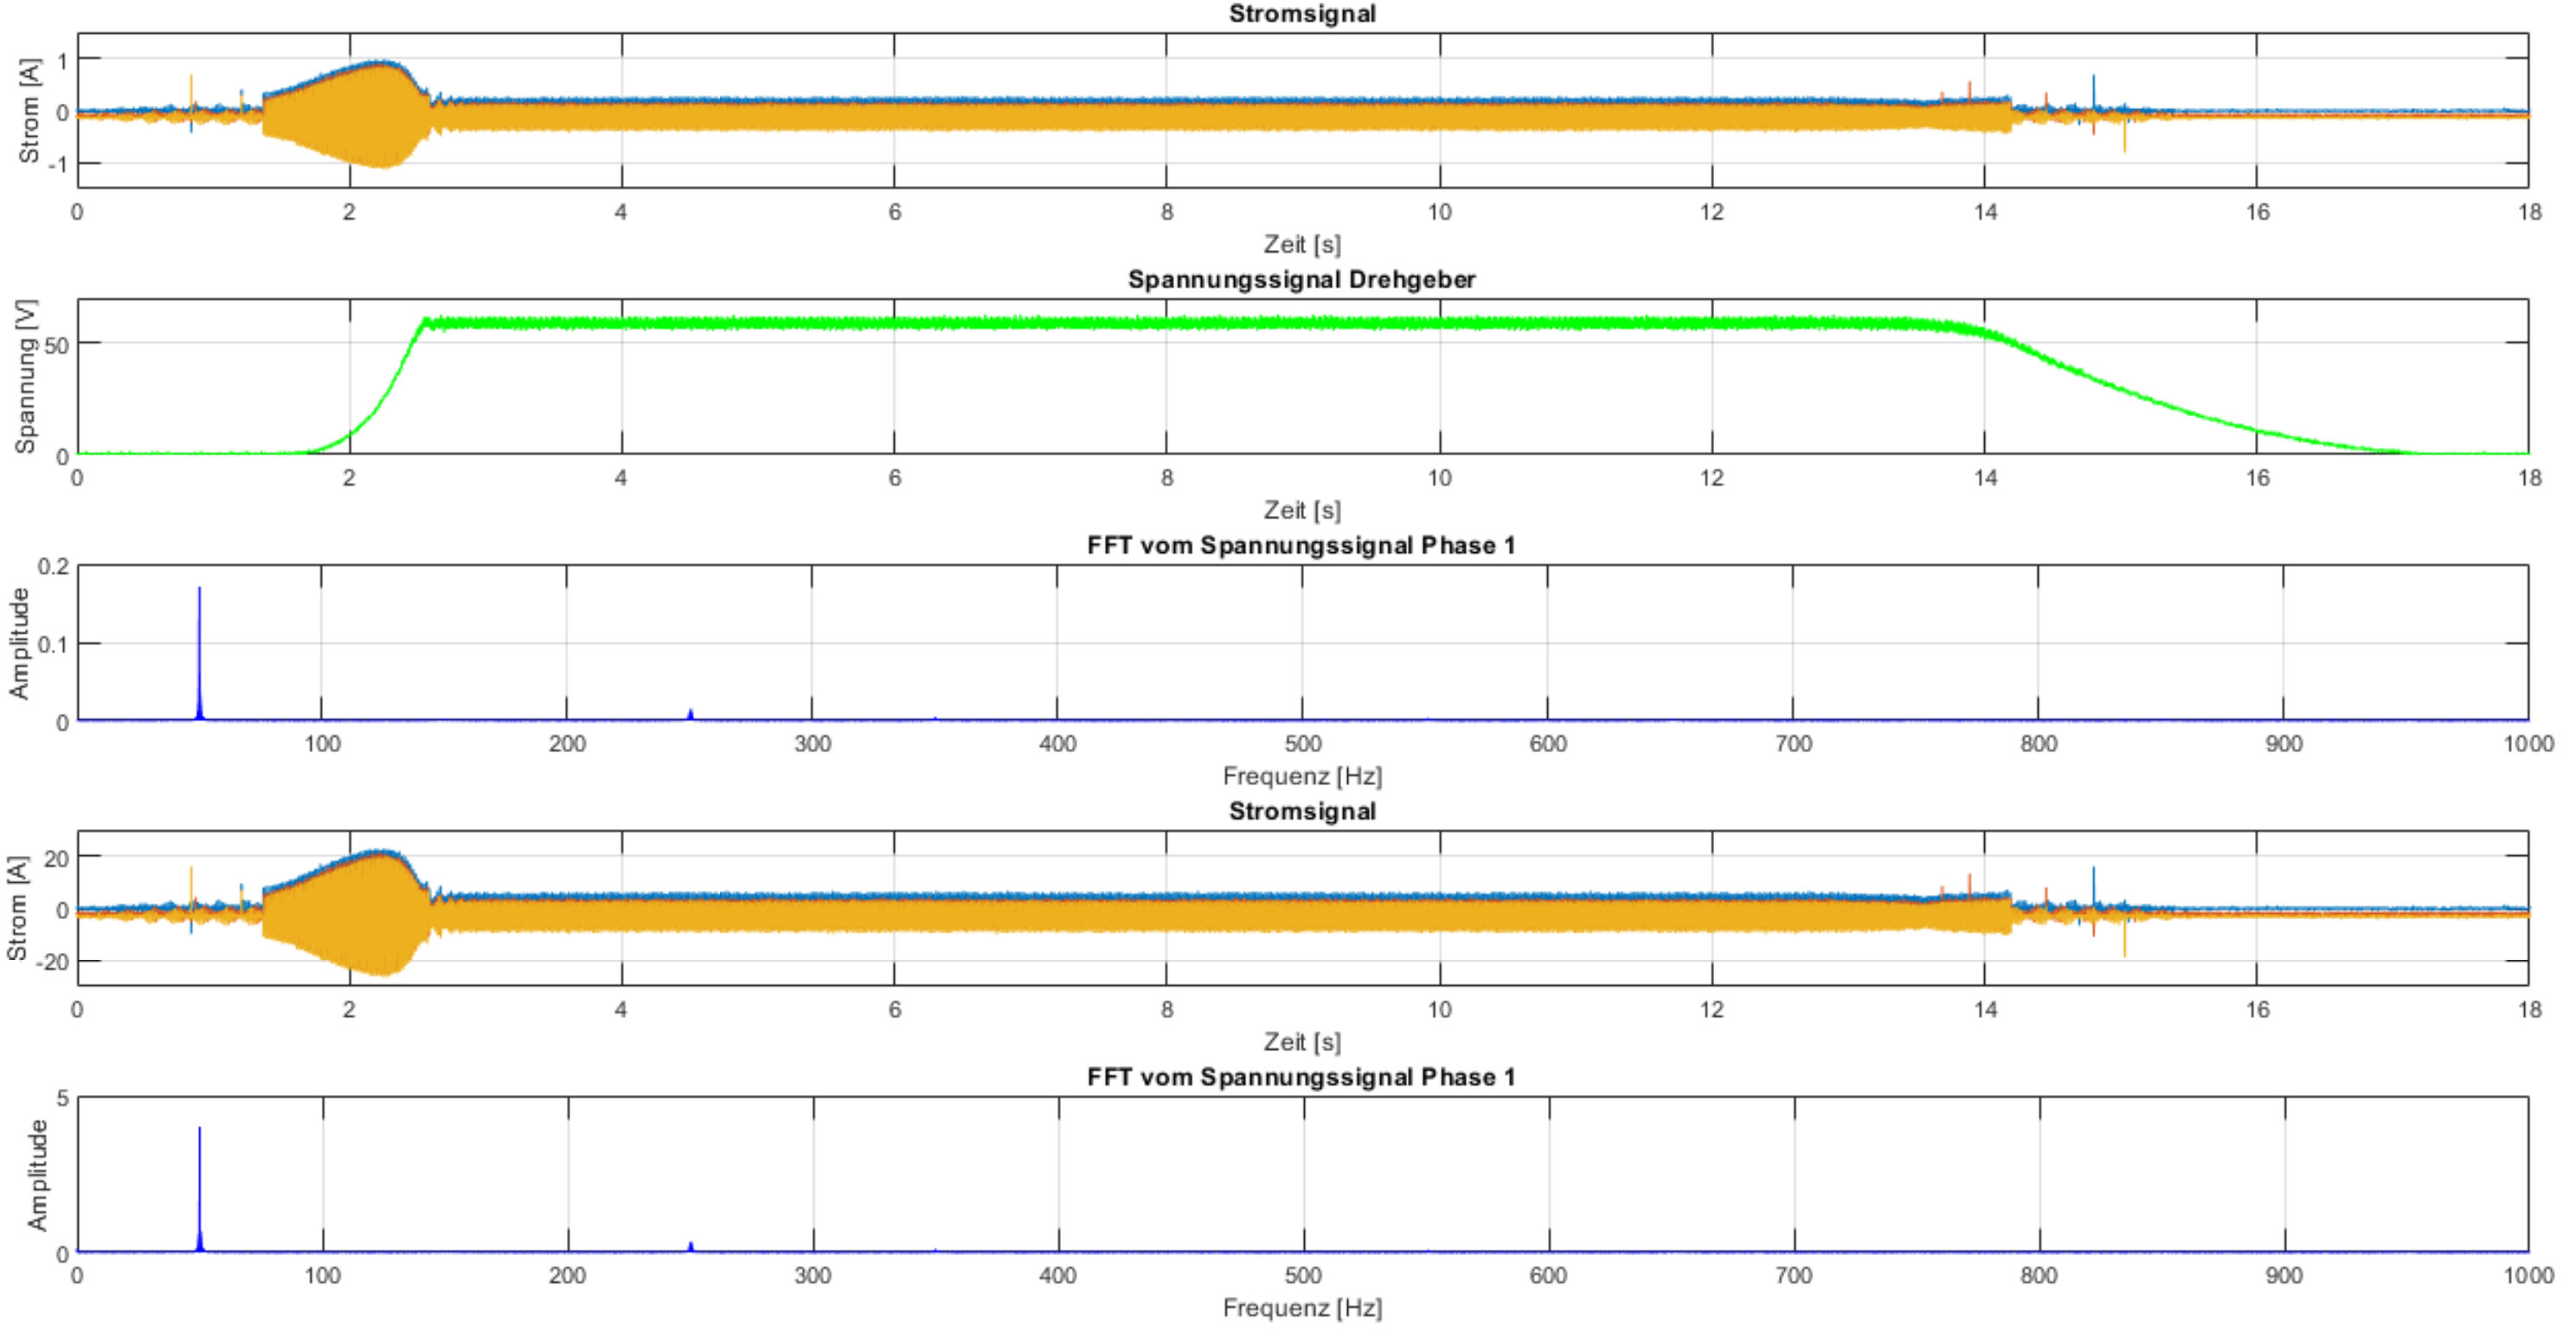
\includegraphics[width=\textwidth]{Messung_ASM_Sanft_langsam_stroeme.png}	
	\caption{Messung mit sanftem Auf- und Absteuern}\label{fig:Mess_Sanft_langsam_stroeme}
\end{figure}

\begin{table}[ht!]
	\centering
	\begin{tabular}{|l|l|l|}
		\hline
		Frequenz {[}Hz{]} & Amplitude {[}A{]} & Verhältnis zur Grundschwingung	\\ \hline
		49.8              & 0.823             & 20.51\%							\\ \hline
		49.9              & 1.064             & 26.51\%							\\ \hline
		49.95             & 1.716             & 42.76\%							\\ \hline
		50                & 4.013             & 100\%							\\ \hline
		50.05             & 1.613             & 40.19\%							\\ \hline
		50.1              & 1.141             & 28.43\%							\\ \hline
		50.2              & 0.878             & 21.88\%							\\ \hline
		250               & 0.28              & 6.98\%							\\ \hline
	\end{tabular}
	\caption{Amplitudenwerte bei den harmonischen Oberschwingungen bei sanftem Auf- und Absteuern}\label{tab:Sanft_langsam_ASM_stroeme}
\end{table}
Wie schon bei der Widerstandsmessung mit dem sanftem Auf- und Absteuern im Kapitel \ref{sec:Sanft_Widerstand_stroeme}, sind bei dieser Messung, mit der ASM, die harmonische Oberschwingungen sehr klein. Sie halten somit die Norm \ref{sec:Stromnormen} ein. In der Tabelle \ref{tab:Sanft_langsam_ASM_stroeme} sind bei verschiedenen Frequenzen die Werte der Amplituden des FFTs aufgelistet.
Die Peaks des Seitenbandes um \SI{50}{Hz} haben ein Verhältnis von bis zu 40\% zur Grundfrequenz.


\newpage
\subsection{Messungen Spannungen}

Damit man die Funktionen des Laboraufbaues mit den Simulationen vergleichen kann, wurden die Spannungen über dem Widerstand und der Asynchronmaschine mit den verschiedenen Ansteuerungsarten gemessen. Dafür wurden die Spannungssignale und das FFT als Grafik und die interessanten Werte der sub-, zwischenharmonischen und harmonischen Schwingungen tabellarisch aufgelistet. Damit auch die Spannungen mit den Normen verglichen werden können, wurde das Verhältnis der verschiedenen Oberschwingungen zur Grundschwingung in Prozent in die Tabellen eingefügt. Da die Phasenanschnittsteureungen die Normen der harmonischen Oberwellen des Stromes nicht einhalten, werden die Spannungssignale bei diesen Verfahren nicht mehr aufgezeigt. Sie sind jedoch im Anhang \ref{sec:Mess_Spannung_Widerstand} ersichtlich. Die Abbildungen in diesem Kapitel sind so aufgebaut, dass zuerst das Spannungssignal über dem Widerstand und anschliessend das daraus berechnete FFT dargestellt wurde.

\subsubsection{Messungen Widerstand}

Zuerst wird die Spannung der Schwingungspaketsteuerung mit einem Duty Cycle von 0.5 und 0.8 über dem ohmschen Widerstand untersucht. Anschliessend betrachtet man das harte und sanfte Auf- und Absteuern der Spannung über dem Widerstand. Da bei diesen Verfahren keine harmonischen Schwingungen auftreten, halten sie die Normen im Kapitel \ref{sec:Spannungsnormen} zu den Harmonischen ein. Die Erkenntnisse zu den Sub- und Zwischenharmonischen werden im Kapitel \ref{sec:Interpretation_Resultate} Interpretation der Resultate erläutert.

\subsubsection*{Schwingungspaket mit Duty Cycle von 0.5}

In Abbildung \ref{fig:Mess_Schwing_50} ist die Schwingungspaketsteuerung mit einem Duty Cycle von 0.5 dargestellt.


\begin{figure}[ht!]
	\centering
	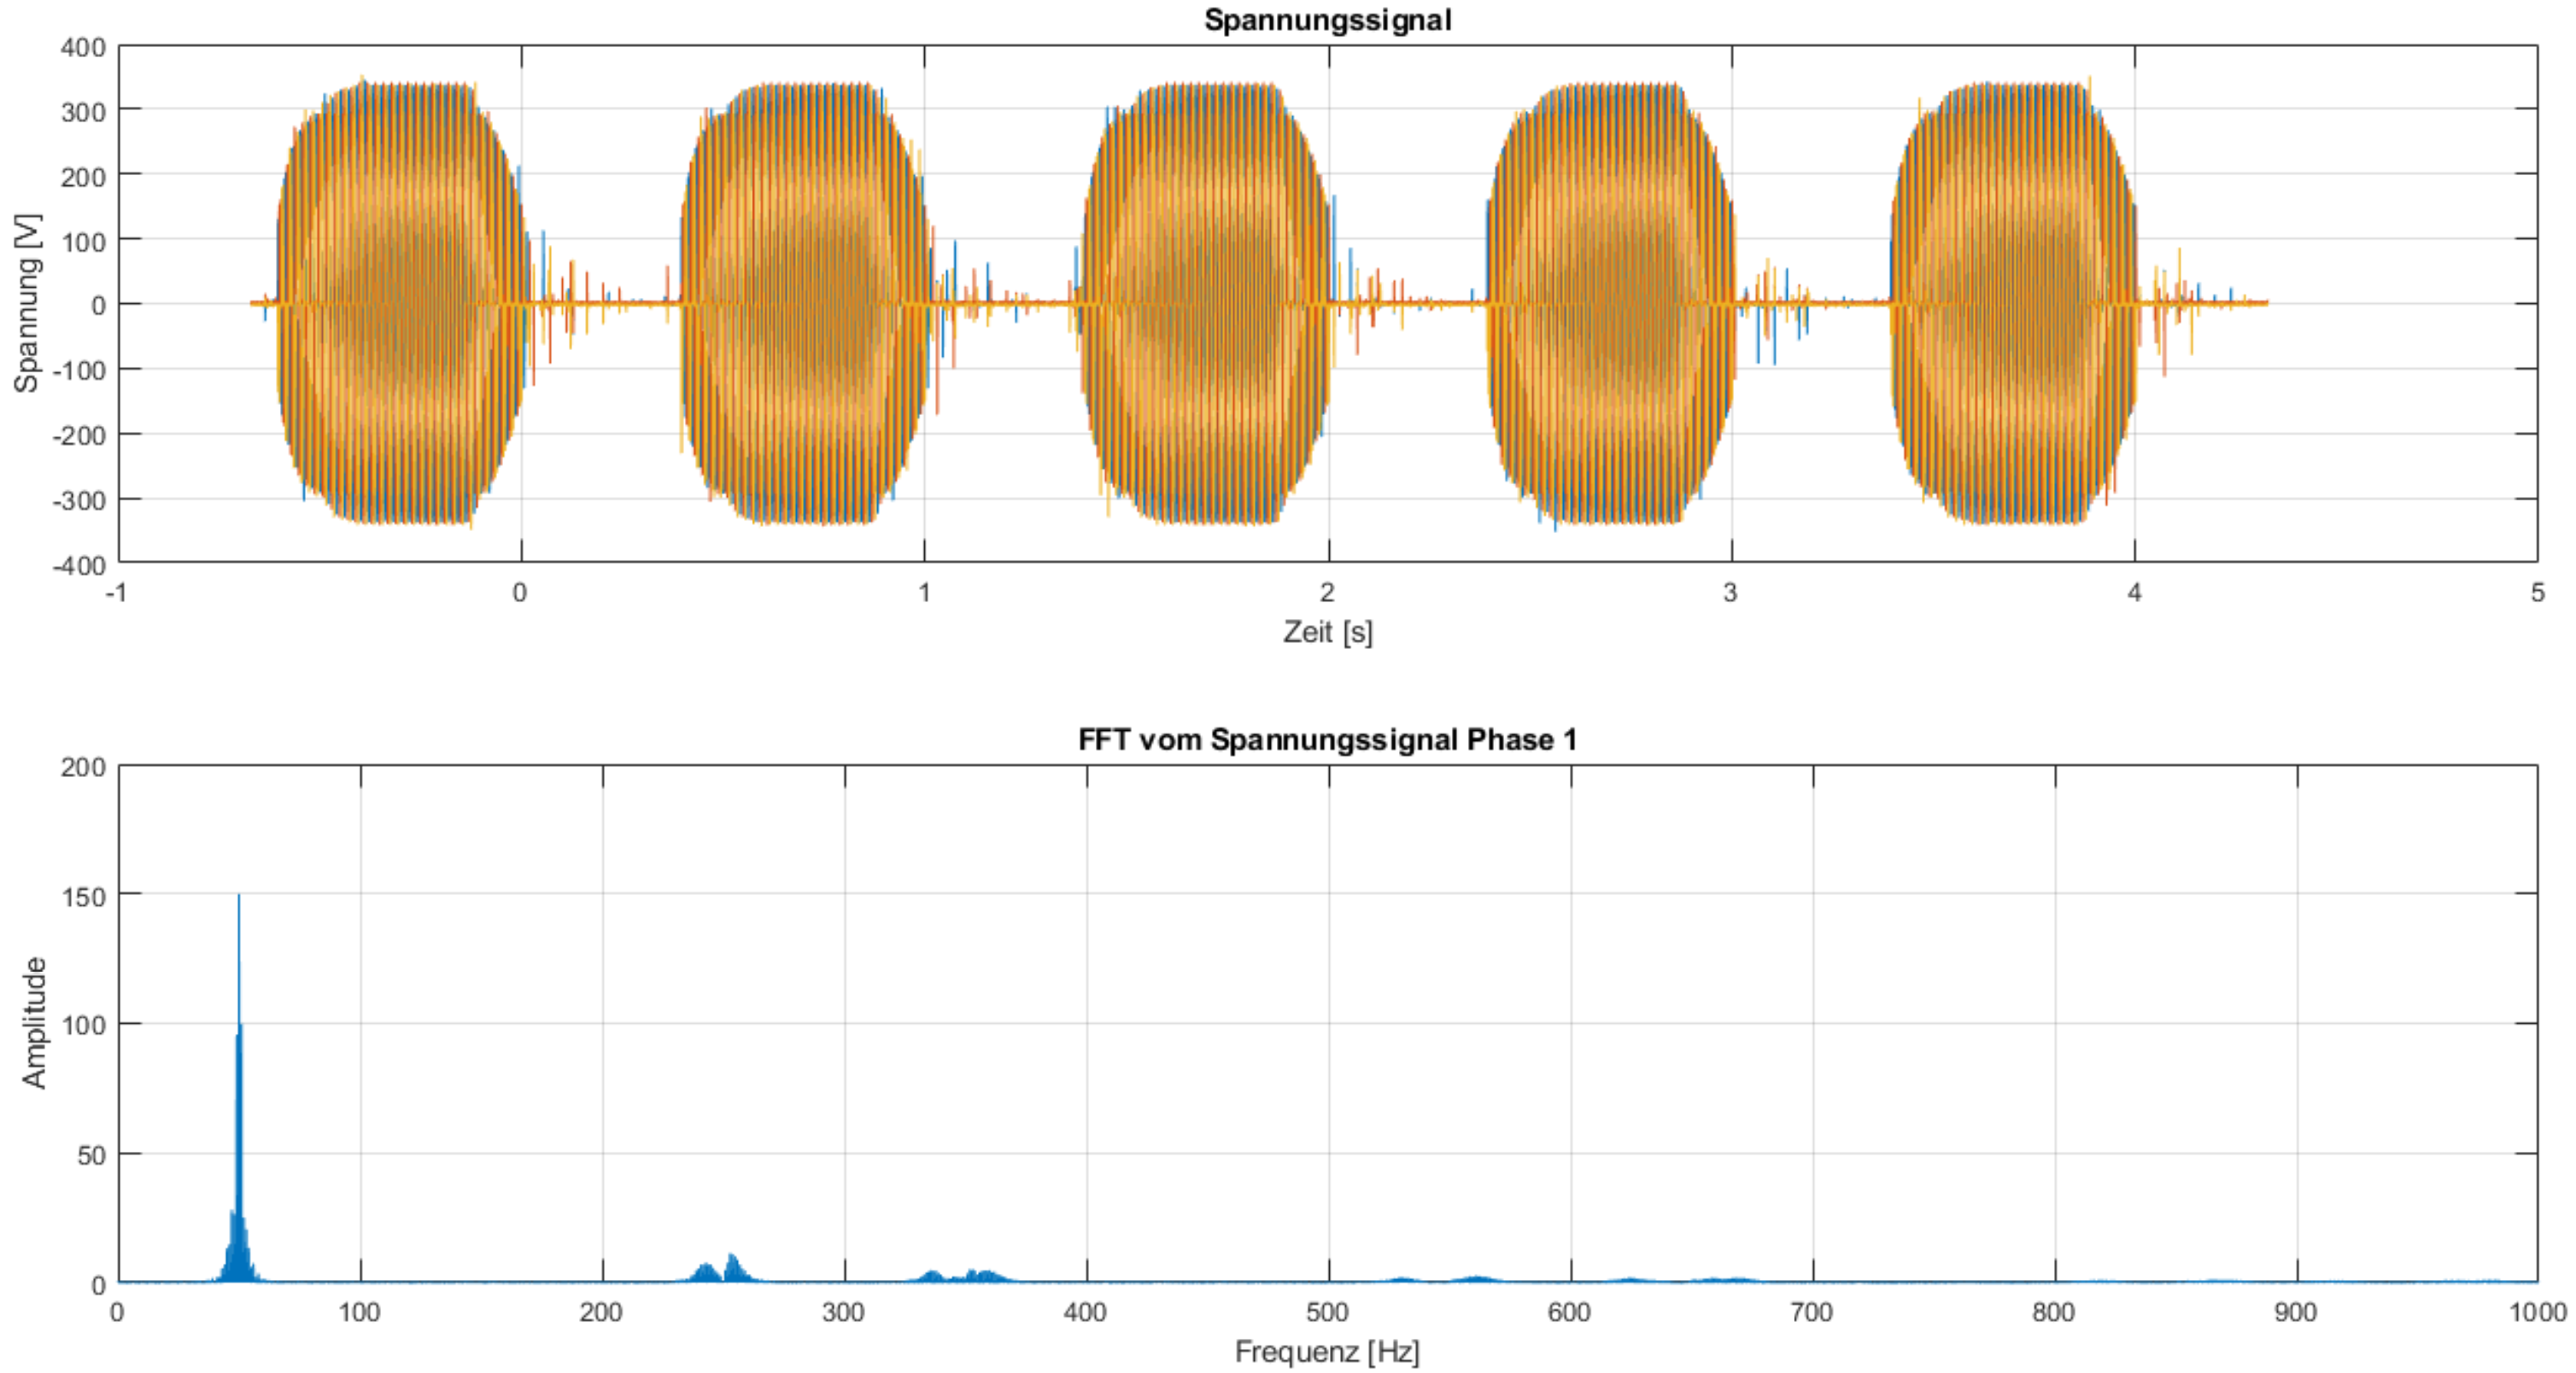
\includegraphics[width=\textwidth]{Messung_Widerstand_Schwing_0_5.png}	
	\caption{Messung mit der Schwingungspaketsteuerung mit einem Duty Cycle von 0.5}\label{fig:Mess_Schwing_50}
\end{figure}


\newpage
\begin{table}[ht!]
	\centering
	\begin{tabular}{|l|l|l|}
		\hline
		Frequenz {[}Hz{]} & Amplitude {[}V{]} & Verhältnis zur Grundschwingung \\ \hline
		46                & 14.7351           & 9.83\%                         \\ \hline
		47                & 28                & 18.68\%                        \\ \hline
		48                & 26.376            & 17.59\%                        \\ \hline
		49                & 95.6              & 63.77\%                        \\ \hline
		50                & 149.92            & 100\%                          \\ \hline
		51                & 99.8              & 66.57\%                        \\ \hline
		52                & 25.134            & 16.76\%                        \\ \hline
		53                & 20.6              & 13.74\%                        \\ \hline
	\end{tabular}
\caption{Amplitudenwerte bei der Frequenzen bei der Schwingungspaketsteuerung mit einem Duty Cycle von 0.5}\label{tab:Mess_Spannung_Schwing_50}
\end{table}

Wie bei den Simulationen im Kapitel \ref{sec:Schwingungspaketsteuerung_Simulation} gezeigt, treten bei der Schwingungspaketsteuerung fast keine harmonischen Oberwellen auf. Bei dem FFT erkennt man, dass das Seitenband bei der Grundschwingung relativ breit ist. In der Tabelle \ref{tab:Mess_Spannung_Schwing_50} sind die Werte der Amplituden der Sub- und Zwischenharmonischen aufgelistet. Dabei wurden die Werte aus dem FFT ausgelesen, welche sich in der Nähe der Grundschwingung von \SI{50}{Hz} befinden und einen hohen Amplitudenwert besitzen. \\
Die Werte der Tabelle \ref{tab:Mess_Spannung_Schwing_50} wurden mit denen des FFTs der Plecs-Simulation verglichen. Die Grafik und die Werte der Messung und der Simulation befinden sich im Anhang \ref{sec:Vergleich_Mess_Sim_Schwing_50}. Dabei wurde festgestellt, dass sich die Kurvenformen der FFT ähnlich aussehen. Jedoch bei näherem betrachten gibt es grosse Unterschiede zwischen den Peak-Werten. In der Simulation schnellen, nach dem Einschalten eines Paketes, die Spannungen sogleich an den Spitzenwert, wobei dies beim Laboraufbau nicht der Fall ist. Deshalb ist bei der Simulation, bei gleicher Zeitdauer, die Spannung länger auf dem Spitzenwert als beim Laboraufbau. Des Weiteren sind alle Bauteile in der Simulation ideal, wobei dies in der Praxis nicht der Fall ist. Deshalb ist auch eine minimale Abweichung des Spitzenwertes ersichtlich. Die Standartabweichung aller aufgeführten Frequenzen beträgt 7.912. Dieser Wert wurde mit Excel berechnet, wobei die Frequenzen als Stichprobe verwendet wurden. \todo{Nochmal überlegen wegen Standartabweichung}



\newpage
\subsubsection*{Schwingungspaketsteuerung mit Duty Cycle von 0.8}
In der Abbildung \ref{fig:Mess_Schwing_80} ist die Schwingungspaketsteuerung mit einem Duty Cycle von 0.8 ersichtlich.
\begin{figure}[ht!]
	\centering
	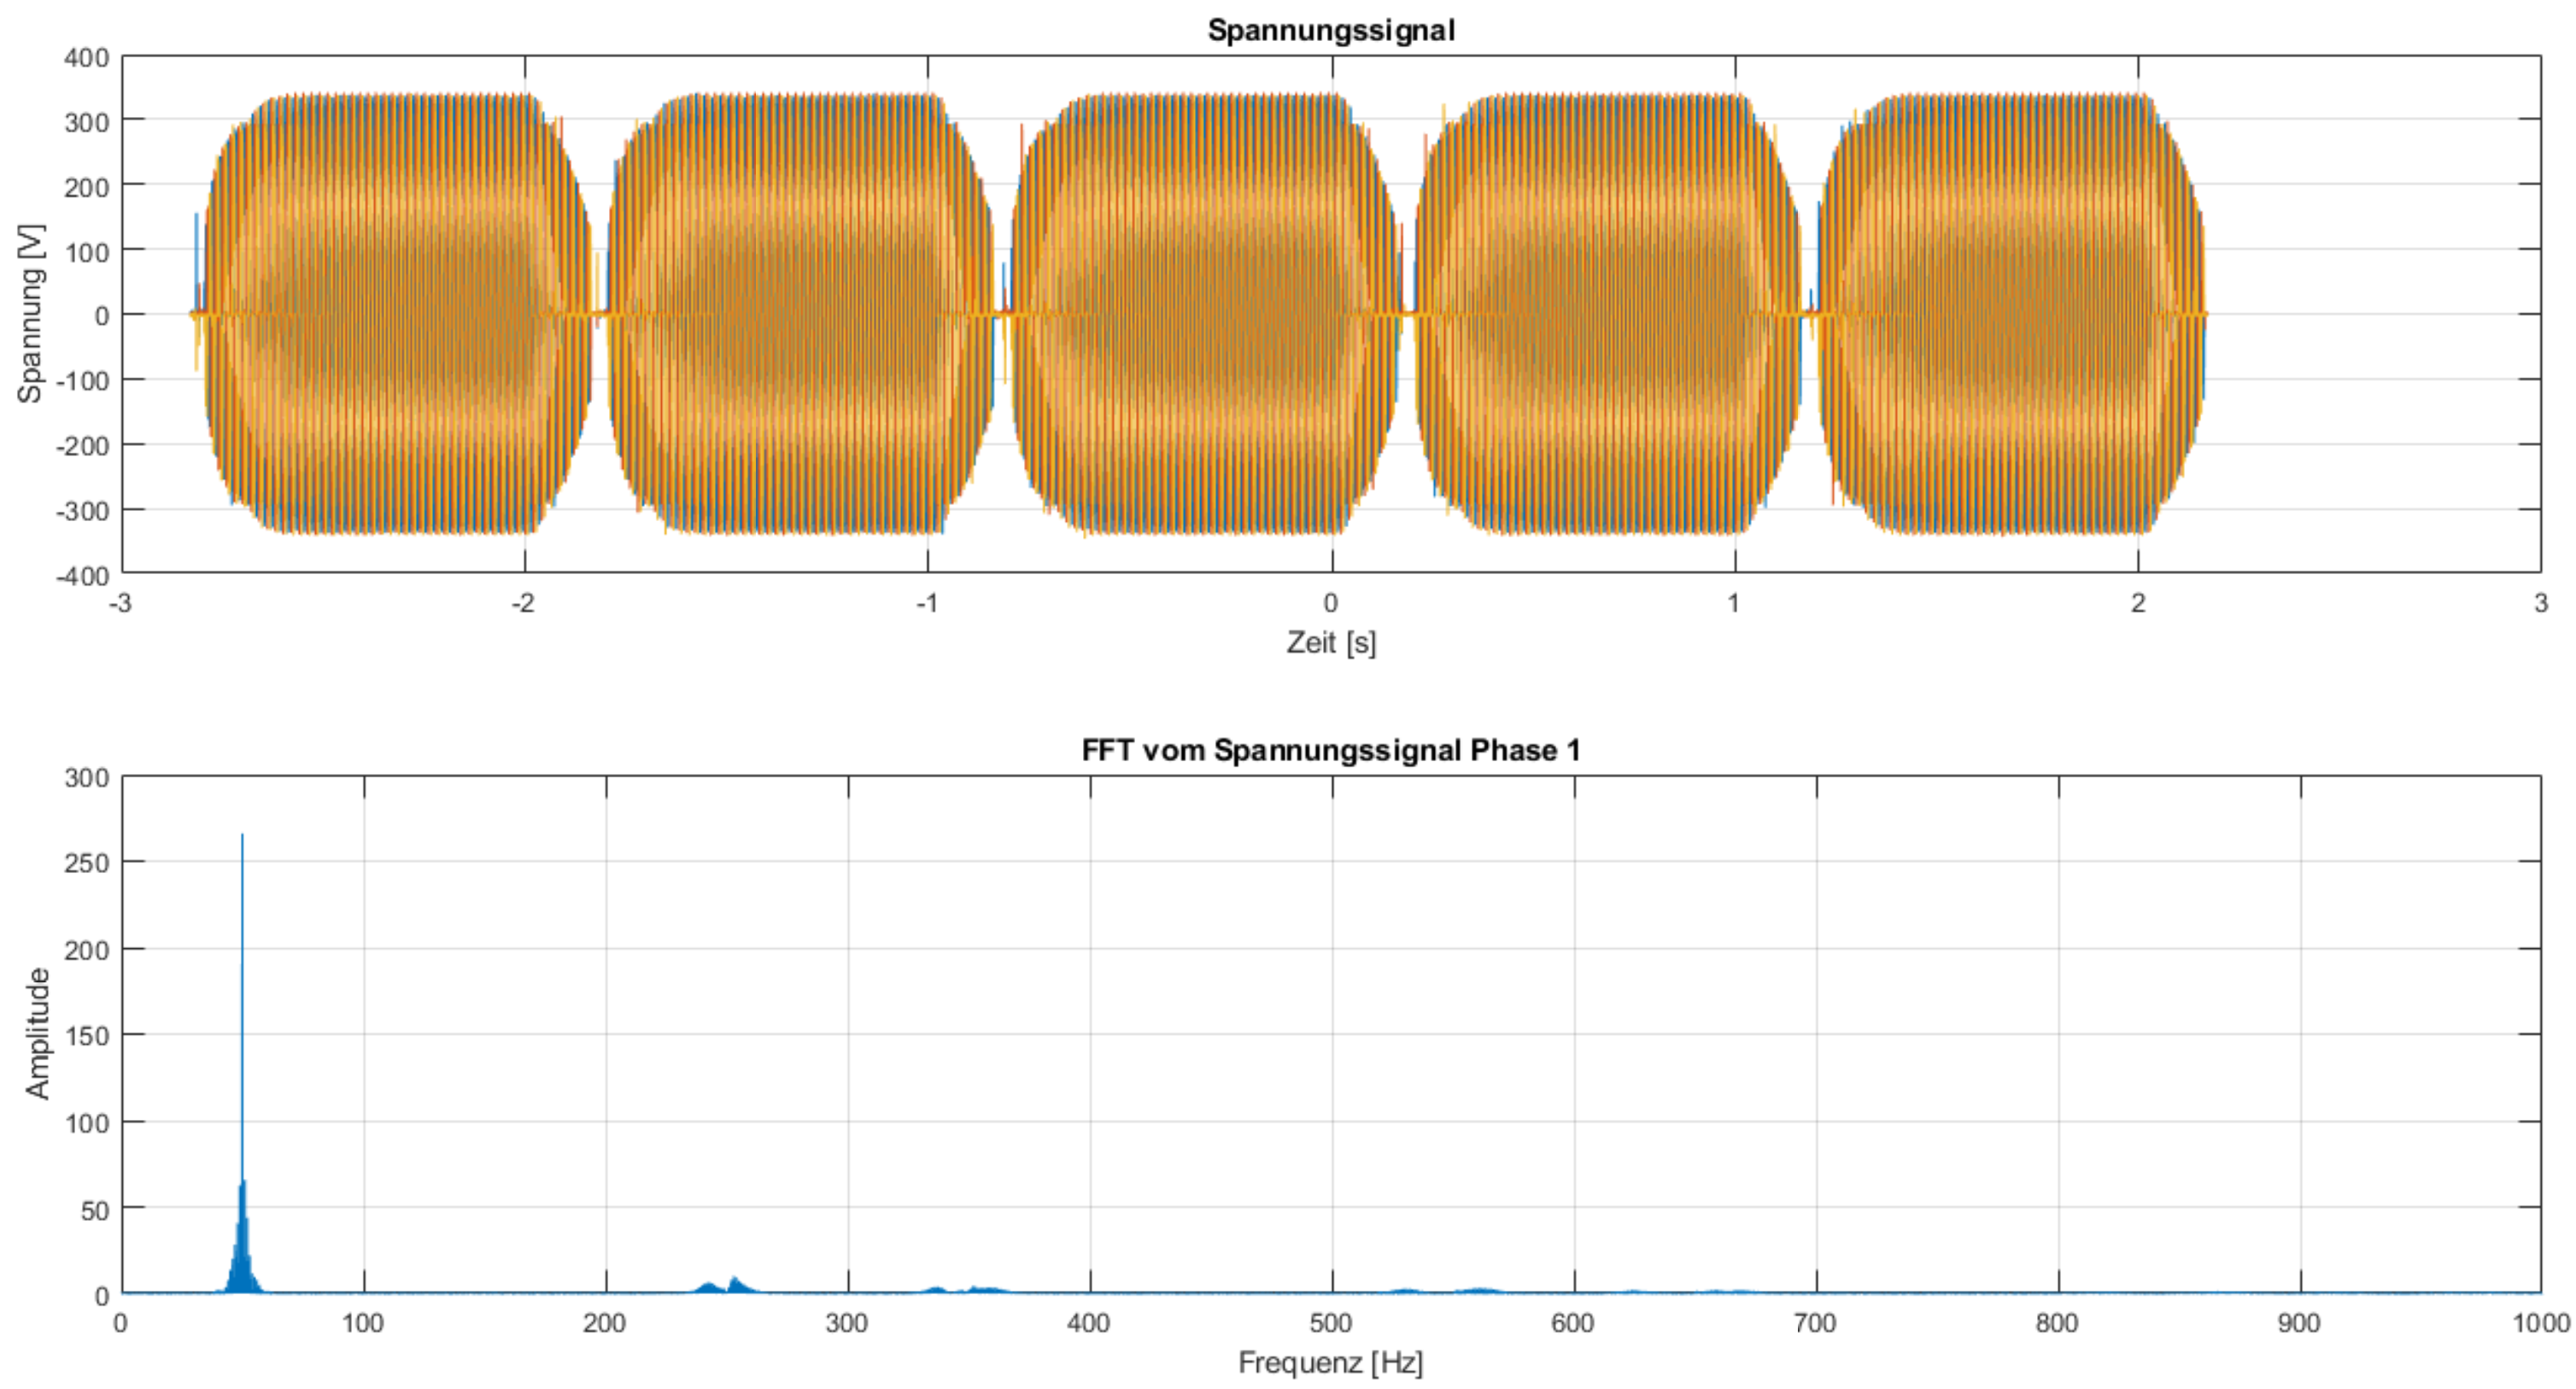
\includegraphics[width=\textwidth]{Messung_Widerstand_Schwing_0_8.png}	
	\caption{Messung mit der Schwingungspaketsteuerung mit einem Duty Cycle von 0.8}\label{fig:Mess_Schwing_80}
\end{figure}


\begin{table}[ht!]
	\centering
	\begin{tabular}{|l|l|l|}
		\hline
		Frequenz {[}Hz{]} & Amplitude {[}V{]} & Verhältnis zur Grundschwingung \\ \hline
		46                & 20.173            & 7.58\%                         \\ \hline
		47                & 28.26             & 10.62\%                        \\ \hline
		48                & 40.576            & 15.26\%                        \\ \hline
		49                & 62.694            & 23.57\%                        \\ \hline
		50                & 265.98            & 100\%                          \\ \hline
		51                & 65.7              & 24.7\%                         \\ \hline
		52                & 43.812            & 16.47\%                        \\ \hline
		53                & 21.939            & 8.25\%                         \\ \hline
	\end{tabular}
\caption{Amplitudenwerte bei der Frequenzen bei Schwingungspaket 80\%}\label{tab:Mess_Spannung_Schwing_80}
\end{table}

Anders als beim Schwingungspaket mit einem Duty Cycle von 0.5, ist bei 0.8 der Peak bei der Grundfrequenz von \SI{50}{Hz} deutlich höher. Das kommt davon, da die Spannung eine längere Zeit auf dem Maximum ist.
In der Tabelle \ref{tab:Mess_Spannung_Schwing_80} befinden sich die Werte der Amplituden und deren Verhältnis zur Grundschwingung.\\
Wie bei der Schwingungspaketsteuerung mit Duty Cycle von 0.5 wurden auch die Resultate der Messung mit 0.8 mit der Simulation verglichen. Die Tabelle mit den Werte und der grafische Vergleich befindet sich im Anhang \ref{sec:Vergleich_Mess_Sim_Schwing_80}. Auch hier gab es Abweichungen bei den verschiedenen Frequenzen zwischen der Simulation und der Messung. Diese waren jedoch bedeutend kleiner als bei der Schwingungspaketsteuerung mit einem Duty Cycle von 0.5. Es resultierte eine Standartabweichung von 2.481. Der Grund, für die niedrigere Abweichung ist, dass die Schwingungspakete eine längere Zeit auf dem Maximum bleiben. Das Hoch- und Herunterfahren haben somit einen kleineren Einfluss auf die Amplitudenwerte. Deshalb ist eine grössere Ähnlichkeit zur Simulation ersichtlich.



\newpage
\subsubsection*{Hartes Auf- und Absteuern}
Die Abbildung \ref{fig:Mess_Sanft} zeigt ein hartes Auf- und Absteuern der Spannung.

\begin{figure}[ht!]
	\centering
	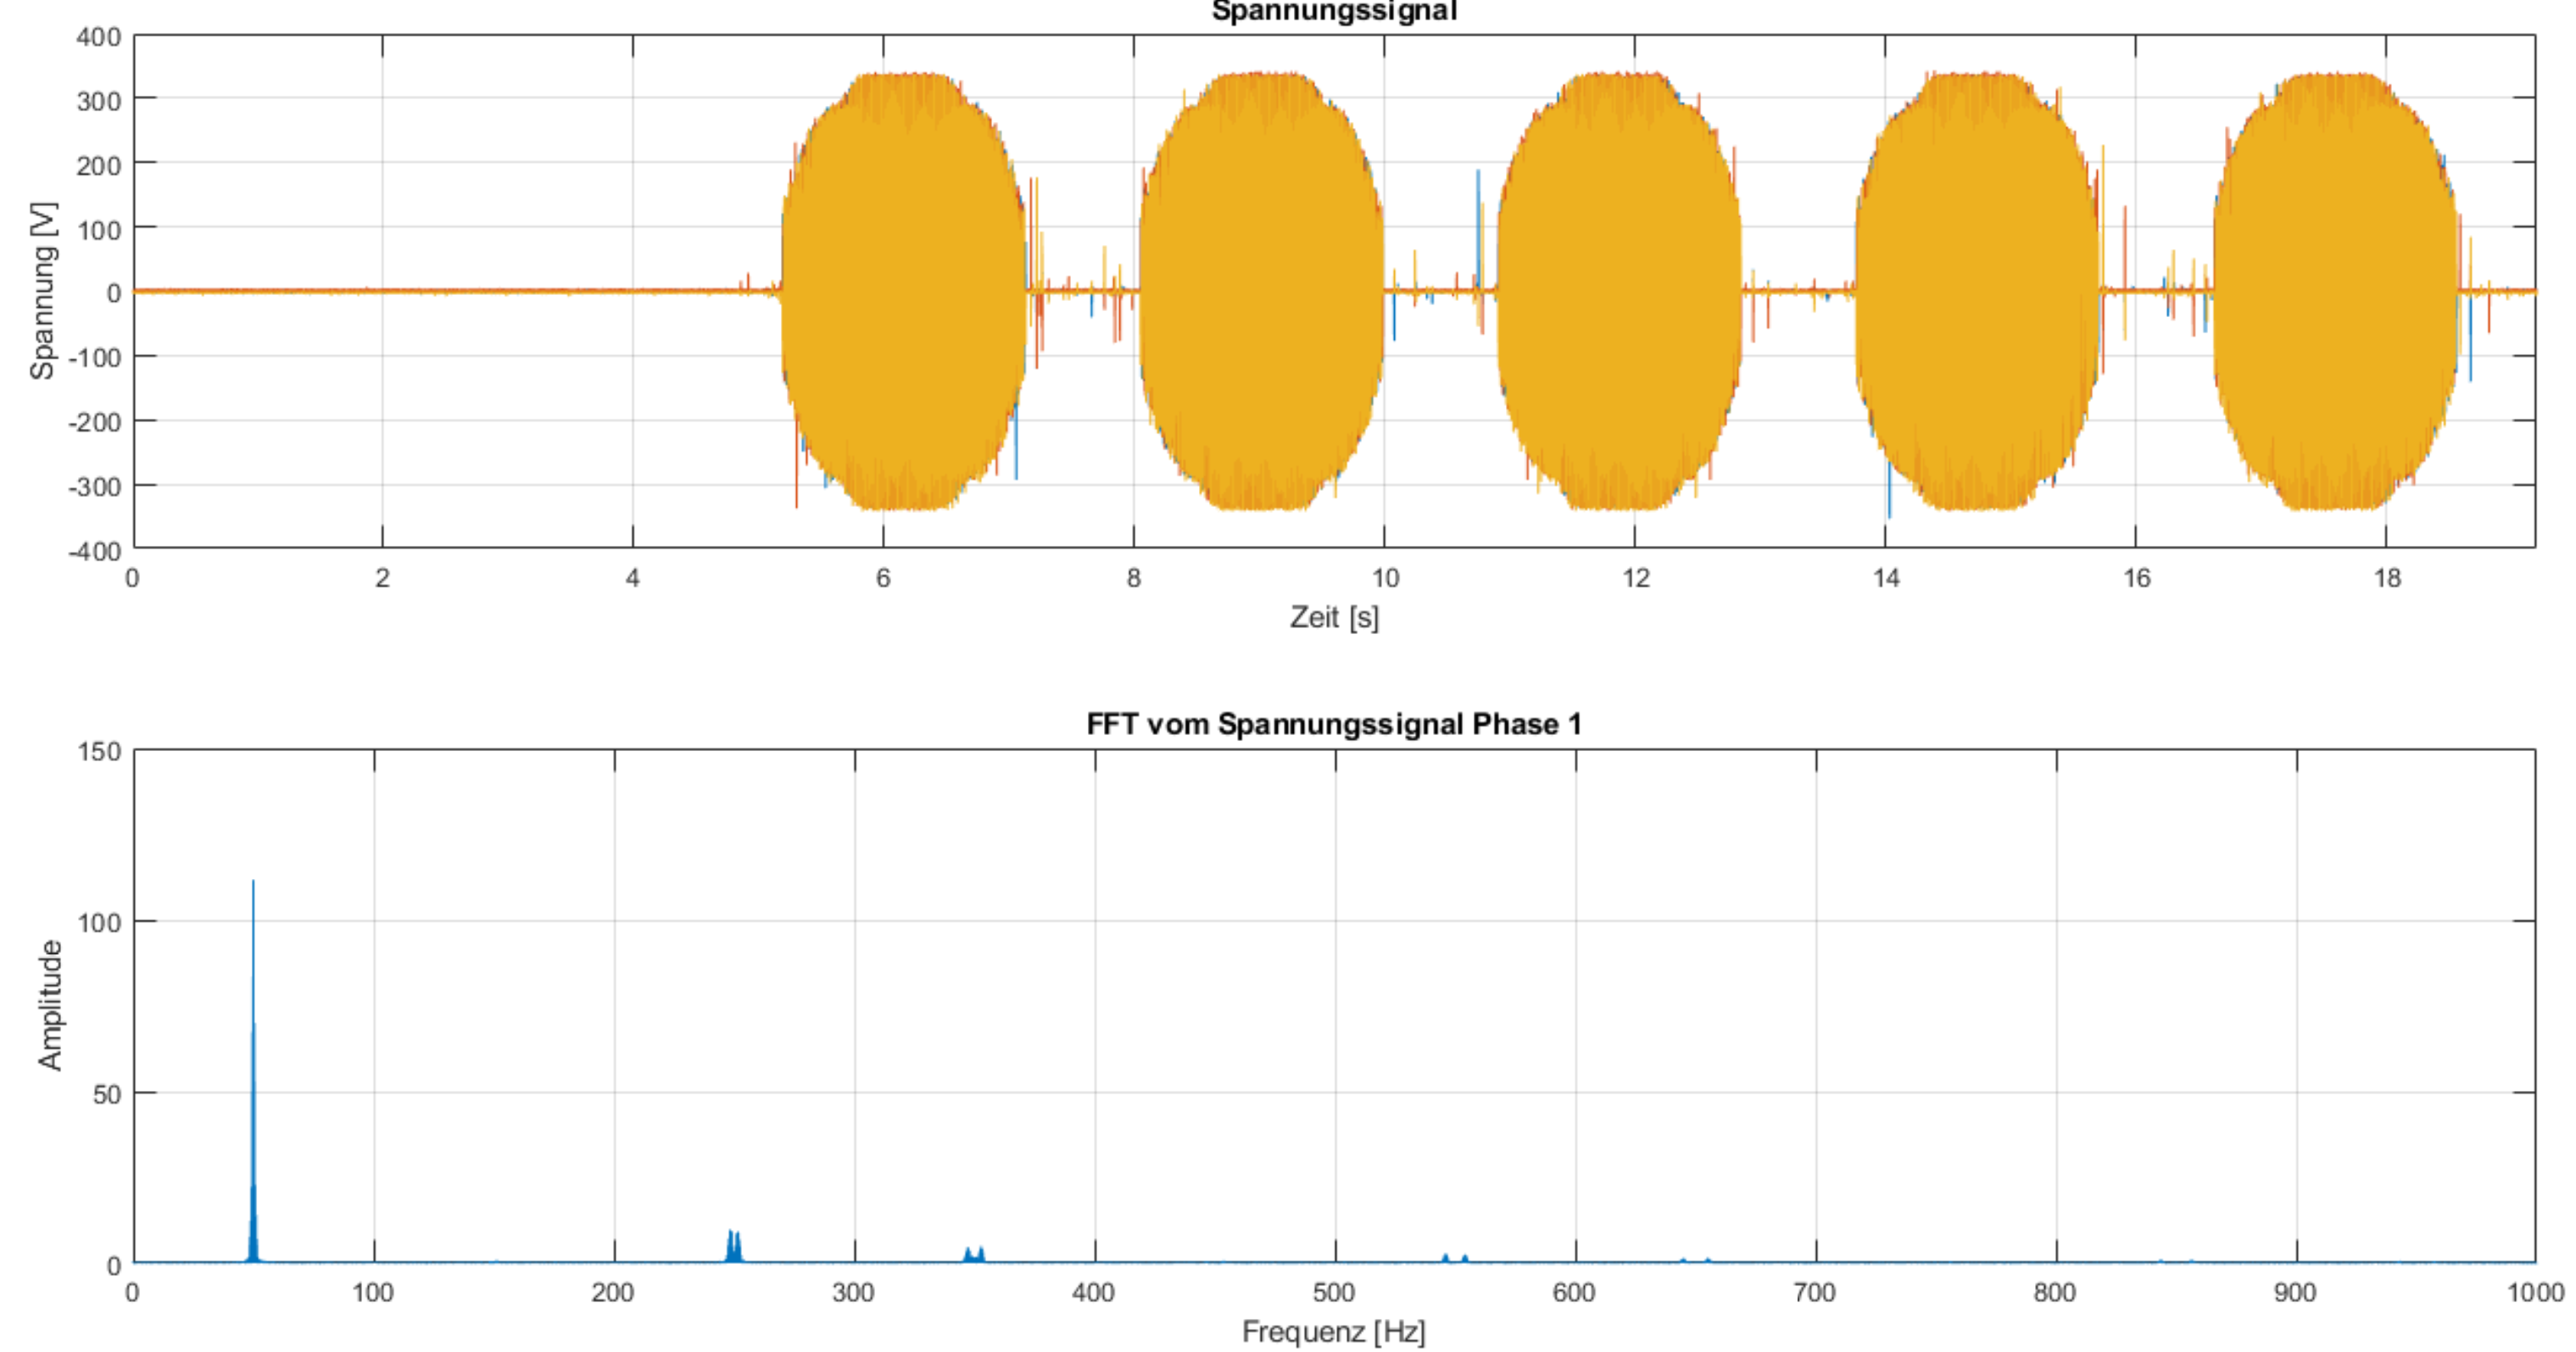
\includegraphics[width=\textwidth]{Mess_Widerstand_AufAb.png}	
	\caption{Messung mit Auf- und Absteuern}\label{fig:Mess_Sanft}
\end{figure}


\begin{table}[ht!]
	\centering
	\begin{tabular}{|l|l|l|}
		\hline
		Frequenz {[}Hz{]} & Amplitude {[}V{]} & Verhältnis zur Grundschwingung \\ \hline
		49.65             & 67.126            & 60.11\%                        \\ \hline
		49.7              & 40.9583           & 36.68\%                        \\ \hline
		50                & 111.6763          & 100\%                          \\ \hline
		50.05             & 58.2021           & 52.12\%                        \\ \hline
		50.35             & 70.0651           & 62.74\%                        \\ \hline
		249               & 9.0297            & 8.09\%                         \\ \hline
		250               & 1.0487            & 0.94\%                         \\ \hline
		251 		      & 1.8206            & 1.63\%                         \\ \hline
	\end{tabular}
\caption{Amplitudenwerte bei der Frequenzen bei hartes Auf- und Absteuern}\label{tab:Mess_Spannung_AufAb_hart}
\end{table}

Für die Tabelle \ref{tab:Mess_Spannung_AufAb_hart} wurden die höchsten Amplitudenwerte bei der Grundschwingung von \SI{50}{Hz} und bei der 5. Harmonische bei \SI{250}{Hz} aufgelistet.
Wie auch bei den Schwingungspaketsteuerungen, tritt bei dem harten Auf- und Absteuern die harmonischen Oberschwingung praktisch nicht mehr auf. Jedoch sind auch hier sub- und zwischenharmonische Oberwellen ersichtlich. Diese betragen bei den Frequenzen \SI{49.65}{Hz} und \SI{50.35}{Hz} über 60\% der Grundschwingung. Bei dem Vergleich des harten Auf- und Absteuern im Laboraufbau und der Simulation wurde ein Unterschied der Signaldauer erkannt. Während bei der Simulation das Auffahren \SI{0.2}{s} dauert, benötigt der Laboraufbau, mit fast \SI{0.8}{s}, deutlich länger. Da der Thyristorsteller nicht schneller reagiert, dauerte es fast \SI{1}{s} bis das nächste Paket hochfährt. Diese Gründe erklären den grossen Unterschied zwischen dem FFT der Simulation und der Messung. Im Kapitel \ref{sec:sanftes_hoch_und_runterfahren} wird das Verhalten von verschieden Anstiegs-Funktionen und die dazu gehörigen FFTs erklärt. Berechnet wurde eine Standartabweichung von 19.812, wobei dieser Wert 2.5 mal grösser ist als die Standartabweichung des Schwingungspaketes mit einem Duty Cycle von 0.5. Der Vergleich mit der Simulation ist im Anhang im Kapitel \ref{sec:Vergleich_Mess_Sim_hart_AufAb} ersichtlich.

\newpage
\subsubsection*{Sanftes Auf- und Absteuern}
Die Abbildung \ref{fig:Mess_Sanft_langsam} zeigt ein sanftes Auf- und Absteuern der Spannung.


\begin{figure}[ht!]
	\centering
	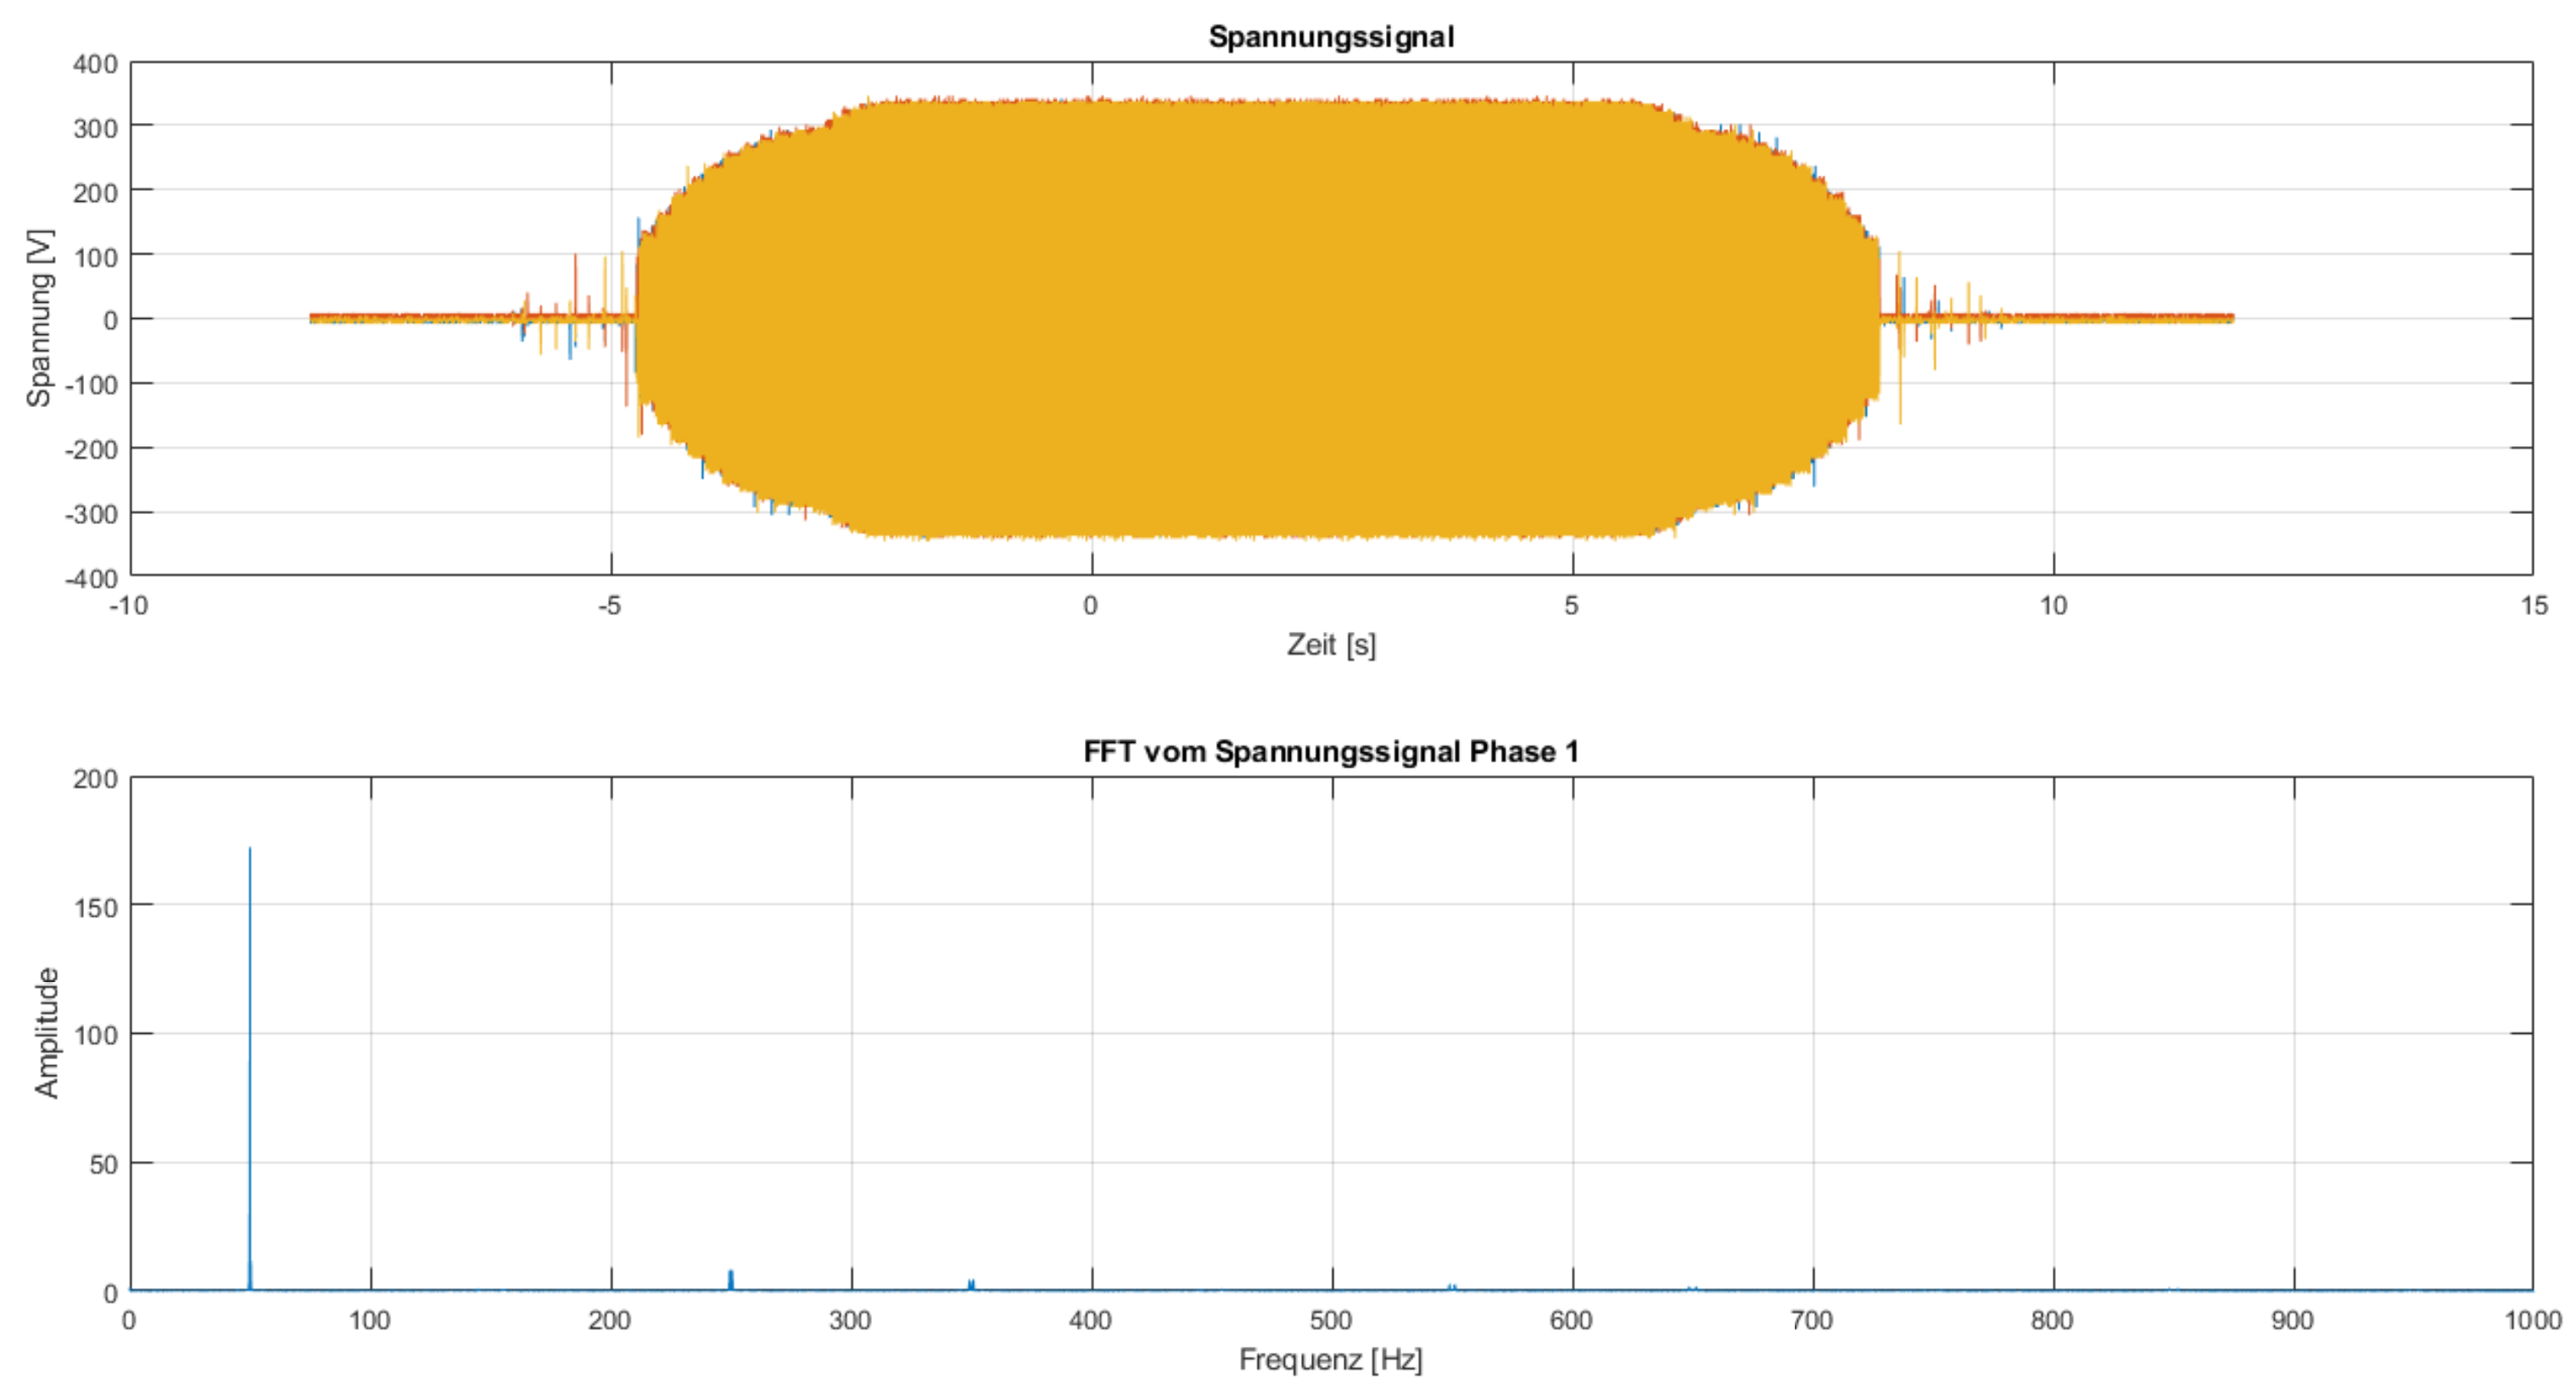
\includegraphics[width=\textwidth]{Messung_Widerstand_Sanft_langsam.png}	
	\caption{Messung mit sanftem Auf- und Absteuern}\label{fig:Mess_Sanft_langsam}
\end{figure}


\begin{table}[ht!]
	\centering
	\begin{tabular}{|l|l|l|}
		\hline
		Frequenz {[}Hz{]} & Amplitude {[}V{]} & Verhältnis zur Grundschwingung \\ \hline
		49.8              & 18.522            & 10.75\%                        \\ \hline
		49.85             & 26.576            & 15.43\%                        \\ \hline
		49.9              & 29.507            & 17.131\%                       \\ \hline
		49.95             & 91.266            & 52.99\%                        \\ \hline
		50                & 172.241           & 100\%                          \\ \hline
		50.05             & 116.719           & 67.76\%                        \\ \hline
		50.1              & 28.629            & 16.62\%                        \\ \hline
		50.15             & 30.076            & 17.46\%                        \\ \hline
		50.2              & 18.72             & 10.87\%                        \\ \hline
		249.6             & 8.183             & 4.75\%                         \\ \hline
		250               & 1.158             & 0.67\%                         \\ \hline
		250.4             & 7.466             & 4.33\%                         \\ \hline
	\end{tabular}
\caption{Amplitudenwerte bei der Frequenzen beim sanften Auf- und Absteuern}\label{tab:Mess_Spannung_AufAb_sanft}
\end{table}

Im visuellen Vergleich mit dem hartem Auf- und Abfahren zeigt das FFT, dass die Frequenzbänder dünner und der Peak bei \SI{50}{Hz} grösser geworden sind. In der Tabelle \ref{tab:Mess_Spannung_AufAb_sanft} sind die höchsten Amplitudenwerte der Frequenzen, die sich in der Nähe der Grundschwingung von \SI{50}{Hz} und der 5. Harmonischen bei \SI{250}{Hz} aufhalten, aufgelistet. Der Vergleich mit der Simulation, befindet sich im Anhang im Kapitel \ref{sec:Vergleich_Mess_Sim_sanft_AufAb}, zeigt grosse Unterschiede der Amplitudenwerte auf. Ein Grund dafür ist, dass die Simulation für das Hoch- und Runterfahren eine Zeitdauer von \SI{0.3}{s} benötigt, wobei sie bei der Messung \SI{3}{s} beträgt. Zusätzlich ist bei der Simulation während \SI{6}{s} die Spannung auf dem Spitzenwert, beim Laboraufbau sind es jedoch \SI{7}{s}.  Berechnet wurde für die Standartabweichung ein Wert von 88.904. Es ist ersichtlich, dass die beiden Funktionen nicht miteinander verglichen werden können, da die Abweichung zu gross ist.


\subsubsection{Messungen Asynchronmaschine}

Auch bei der Asynchronmaschine wurden die verschiedenen Ansteuerungsarten, Phasenanschnitt mit 60\textdegree \hspace{0.02cm} und 90\textdegree \hspace{0.02cm}, Schwingungspaket mit Duty Cycle von 0.5 und 0.8 und dem harten und sanften Auf- und Absteuern durchgeführt. Dabei stellte man fest, dass sich die Schwingungspaketsteuerungen und das harte Auf- und Absteuern nicht für einen Asynchronmotor eignen. Der Motor fährt zu schnell Hinauf und Hinunter und befindet sich nie in einem geeigneten stationären Zustand. Deshalb verzichtete man bei der Messung auf diese Verfahren. Der Aufbau der Abbildungen und Tabellen ist gleich wie bei dem Widerstand.

\subsubsection*{Phasenanschnitt 60\textdegree}

Bei der Abbildung \ref{fig:Mess_ASM_Phas60} verwendete man einen Phasenanschnittswinkel von 60\textdegree.

\begin{figure}[ht!]
	\centering
	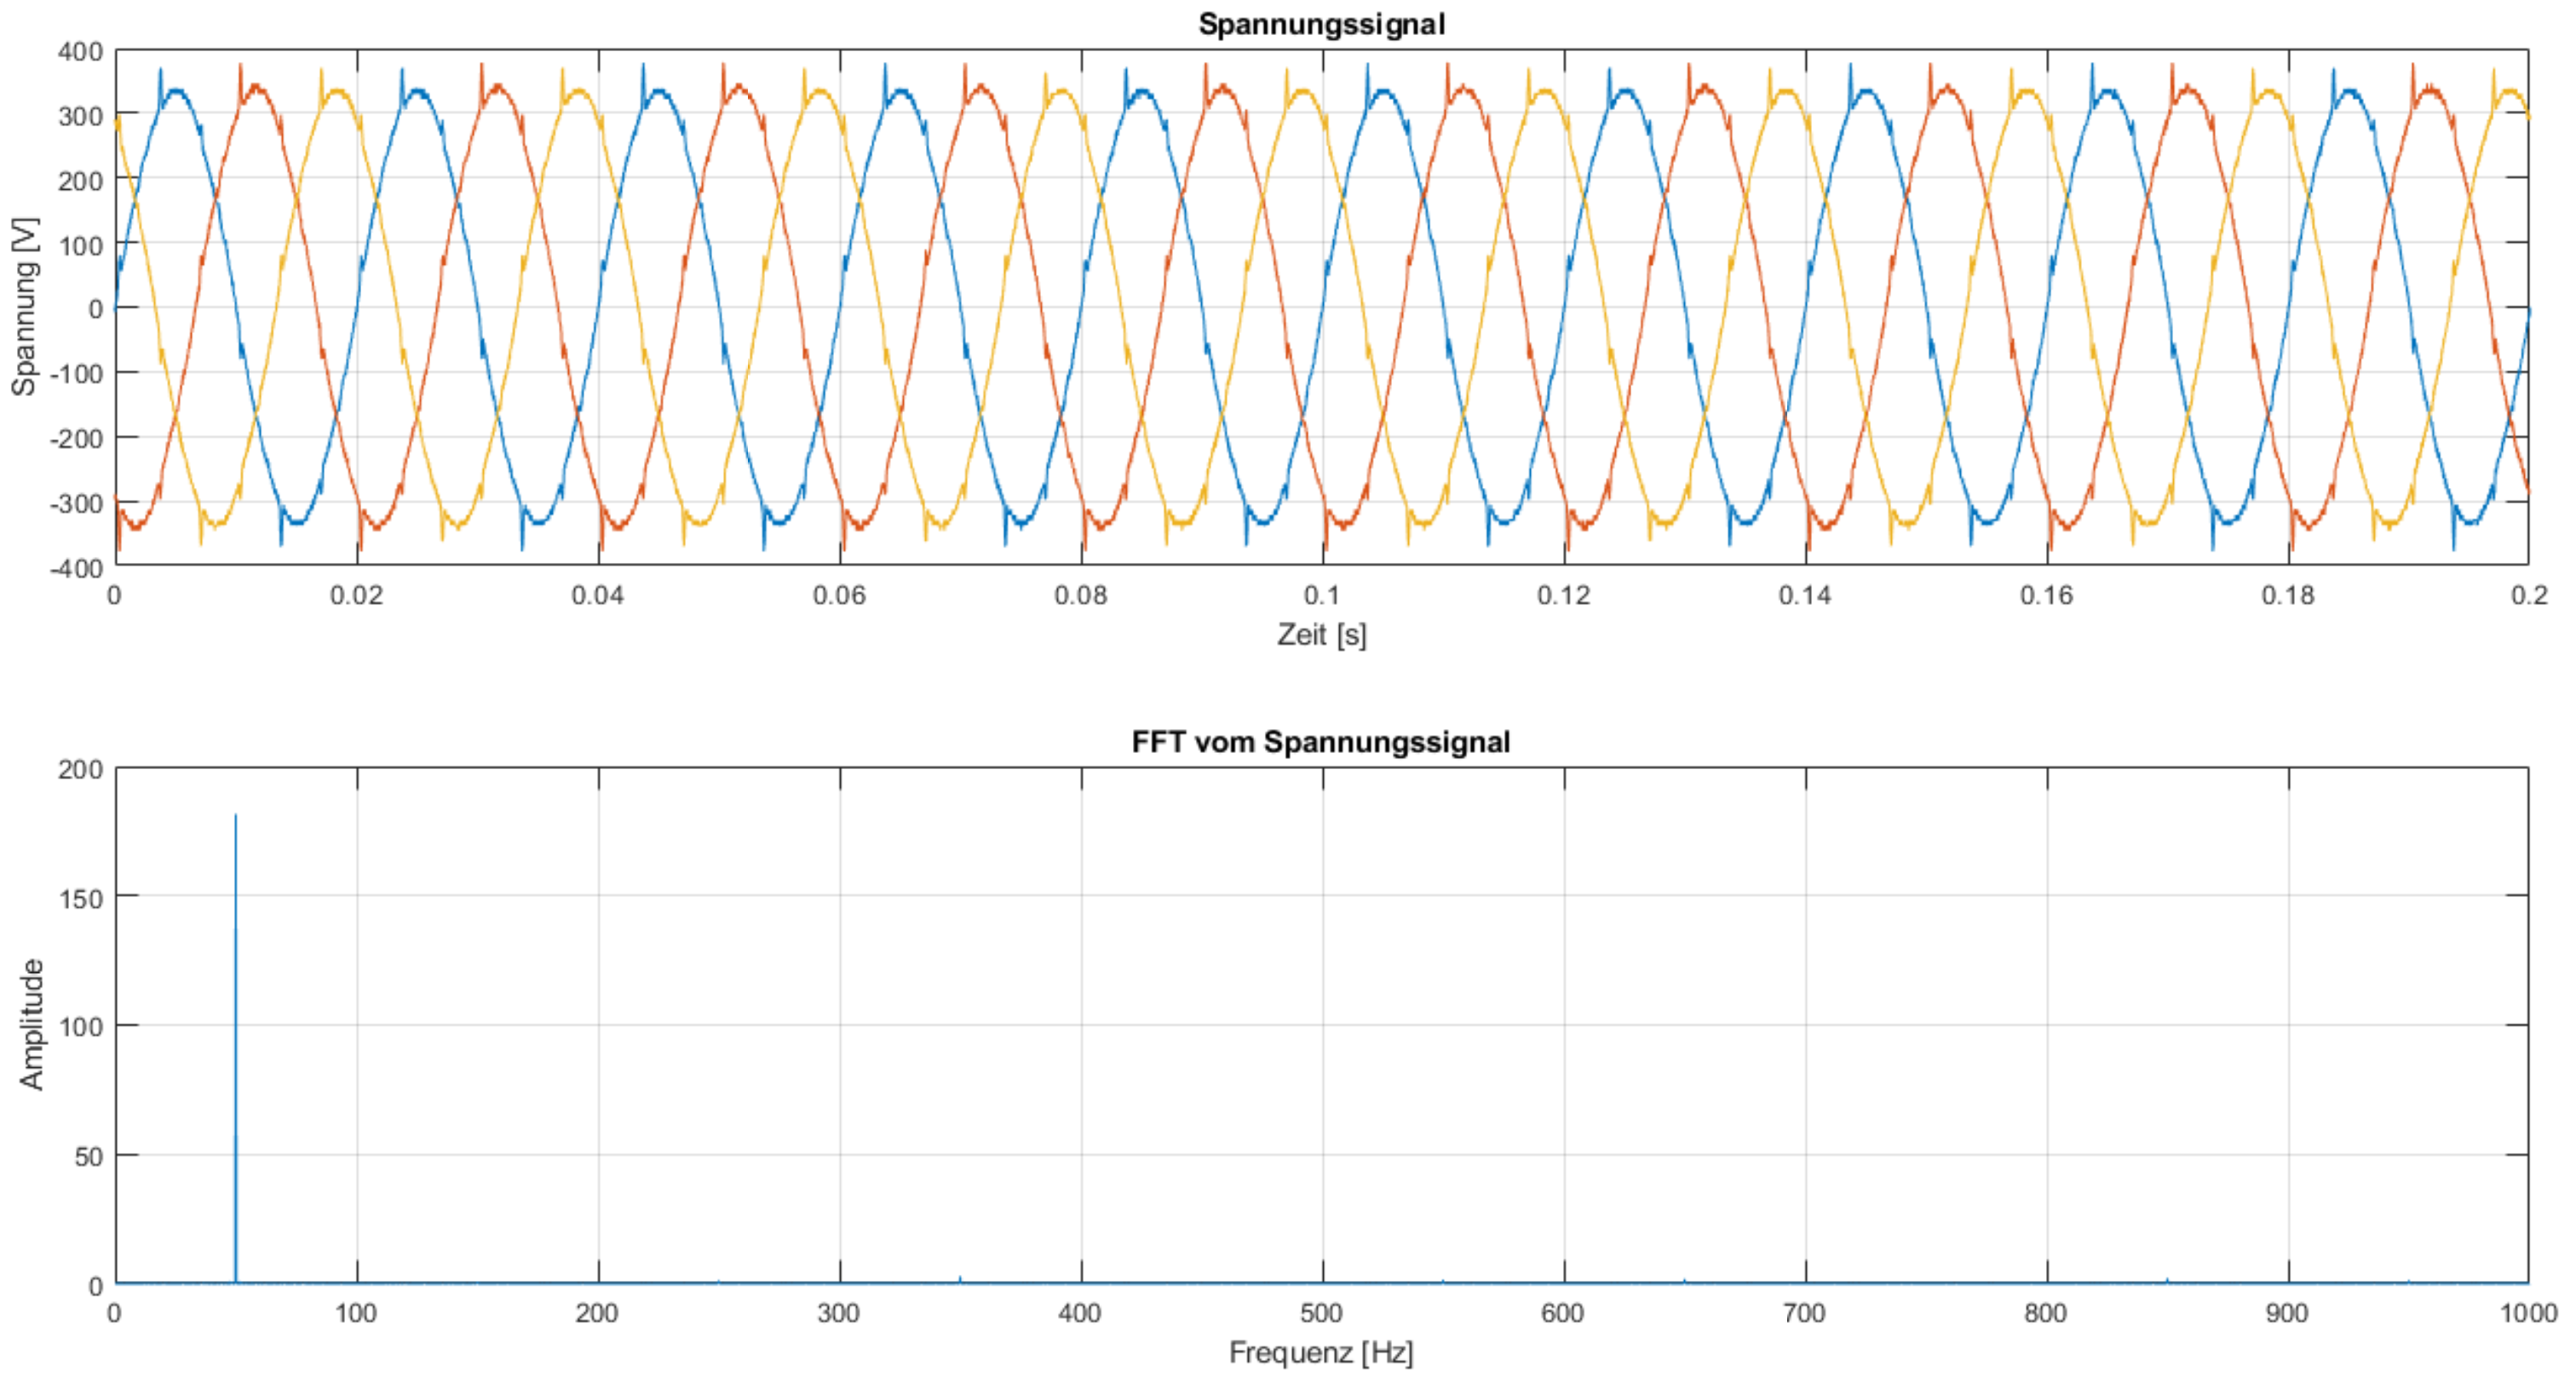
\includegraphics[width=\textwidth]{Messung_ASM_Phas_60grad.png}	
	\caption{Messung mit Phasenanschnitt 60\textdegree}\label{fig:Mess_ASM_Phas60}
\end{figure}


\newpage
\begin{table}[ht!]
	\centering
	\begin{tabular}{|l|l|l|}
		\hline
		Oberschwingungsordnung & Amplitude {[}V{]} & Verhältnis zur Grundschwingung \\ \hline
		1                      & 181.5519          & 100\%                          \\ \hline
		5                      & 1.1065            & 0.61\%                         \\ \hline
		7                      & 2.8728            & 1.58\%                         \\ \hline
		11                     & 1.4537            & 0.8\%                          \\ \hline
	\end{tabular}
\caption{Amplitudenwerte bei der Frequenzen bei Phasenanschnitt 60\textdegree}\label{tab:Mess_Spannung_ASM_Phas60}
\end{table}

Anders als beim Phasenanschnitt von 60\textdegree\hspace{0.02cm} mit dem ohmschen Widerstand, treten bei dem Asynchronmotor fast keine harmonischen Oberschwingungen auf. Da diese Peaks im FFT nicht ersichtlich sind, wurden die Amplituden der Oberschwingungen bis zur 11. Ordnung in der Tabelle \ref{tab:Mess_Spannung_ASM_Phas60} aufgeführt. 
Beim Ansteuern mit dem Winkel von 60\textdegree \hspace{0.02cm} wurde bemerkt, dass die Maschine bereits mit maximaler Drehzahl dreht. Es macht bei den Spannungssignalen keinen Unterschied ob die ASM mit einem Winkel von 60\textdegree \hspace{0.02cm} oder 0\textdegree \hspace{0.02cm} angesteuert wird. Anders als beim Phasenanschnitt mit 60\textdegree\hspace{0.02cm} bei ohmscher Last, sind mit dem gleichen Anschnitswinkel bei der ASM keine Sub- und Zwischenharmonische in der Nähe der Grundfrequenz ersichtlich. Im Verhältnis zur Grundschwingung hat die 7. Ordnung die maximale Abweichung von 1.58\%. Die Werte der harmonischen Schwingungen halten somit die Normen in der Tabelle \ref{tab:kompatibilitätsstufen} ein. 

\newpage
\subsubsection*{Phasenanschnitt 90\textdegree}
Die Abbildung \ref{fig:Mess_ASM_Phas90} zeigt eine Steuerung mit einem Phasenanschnitt von 90\textdegree.

\begin{figure}[ht!]
	\centering
	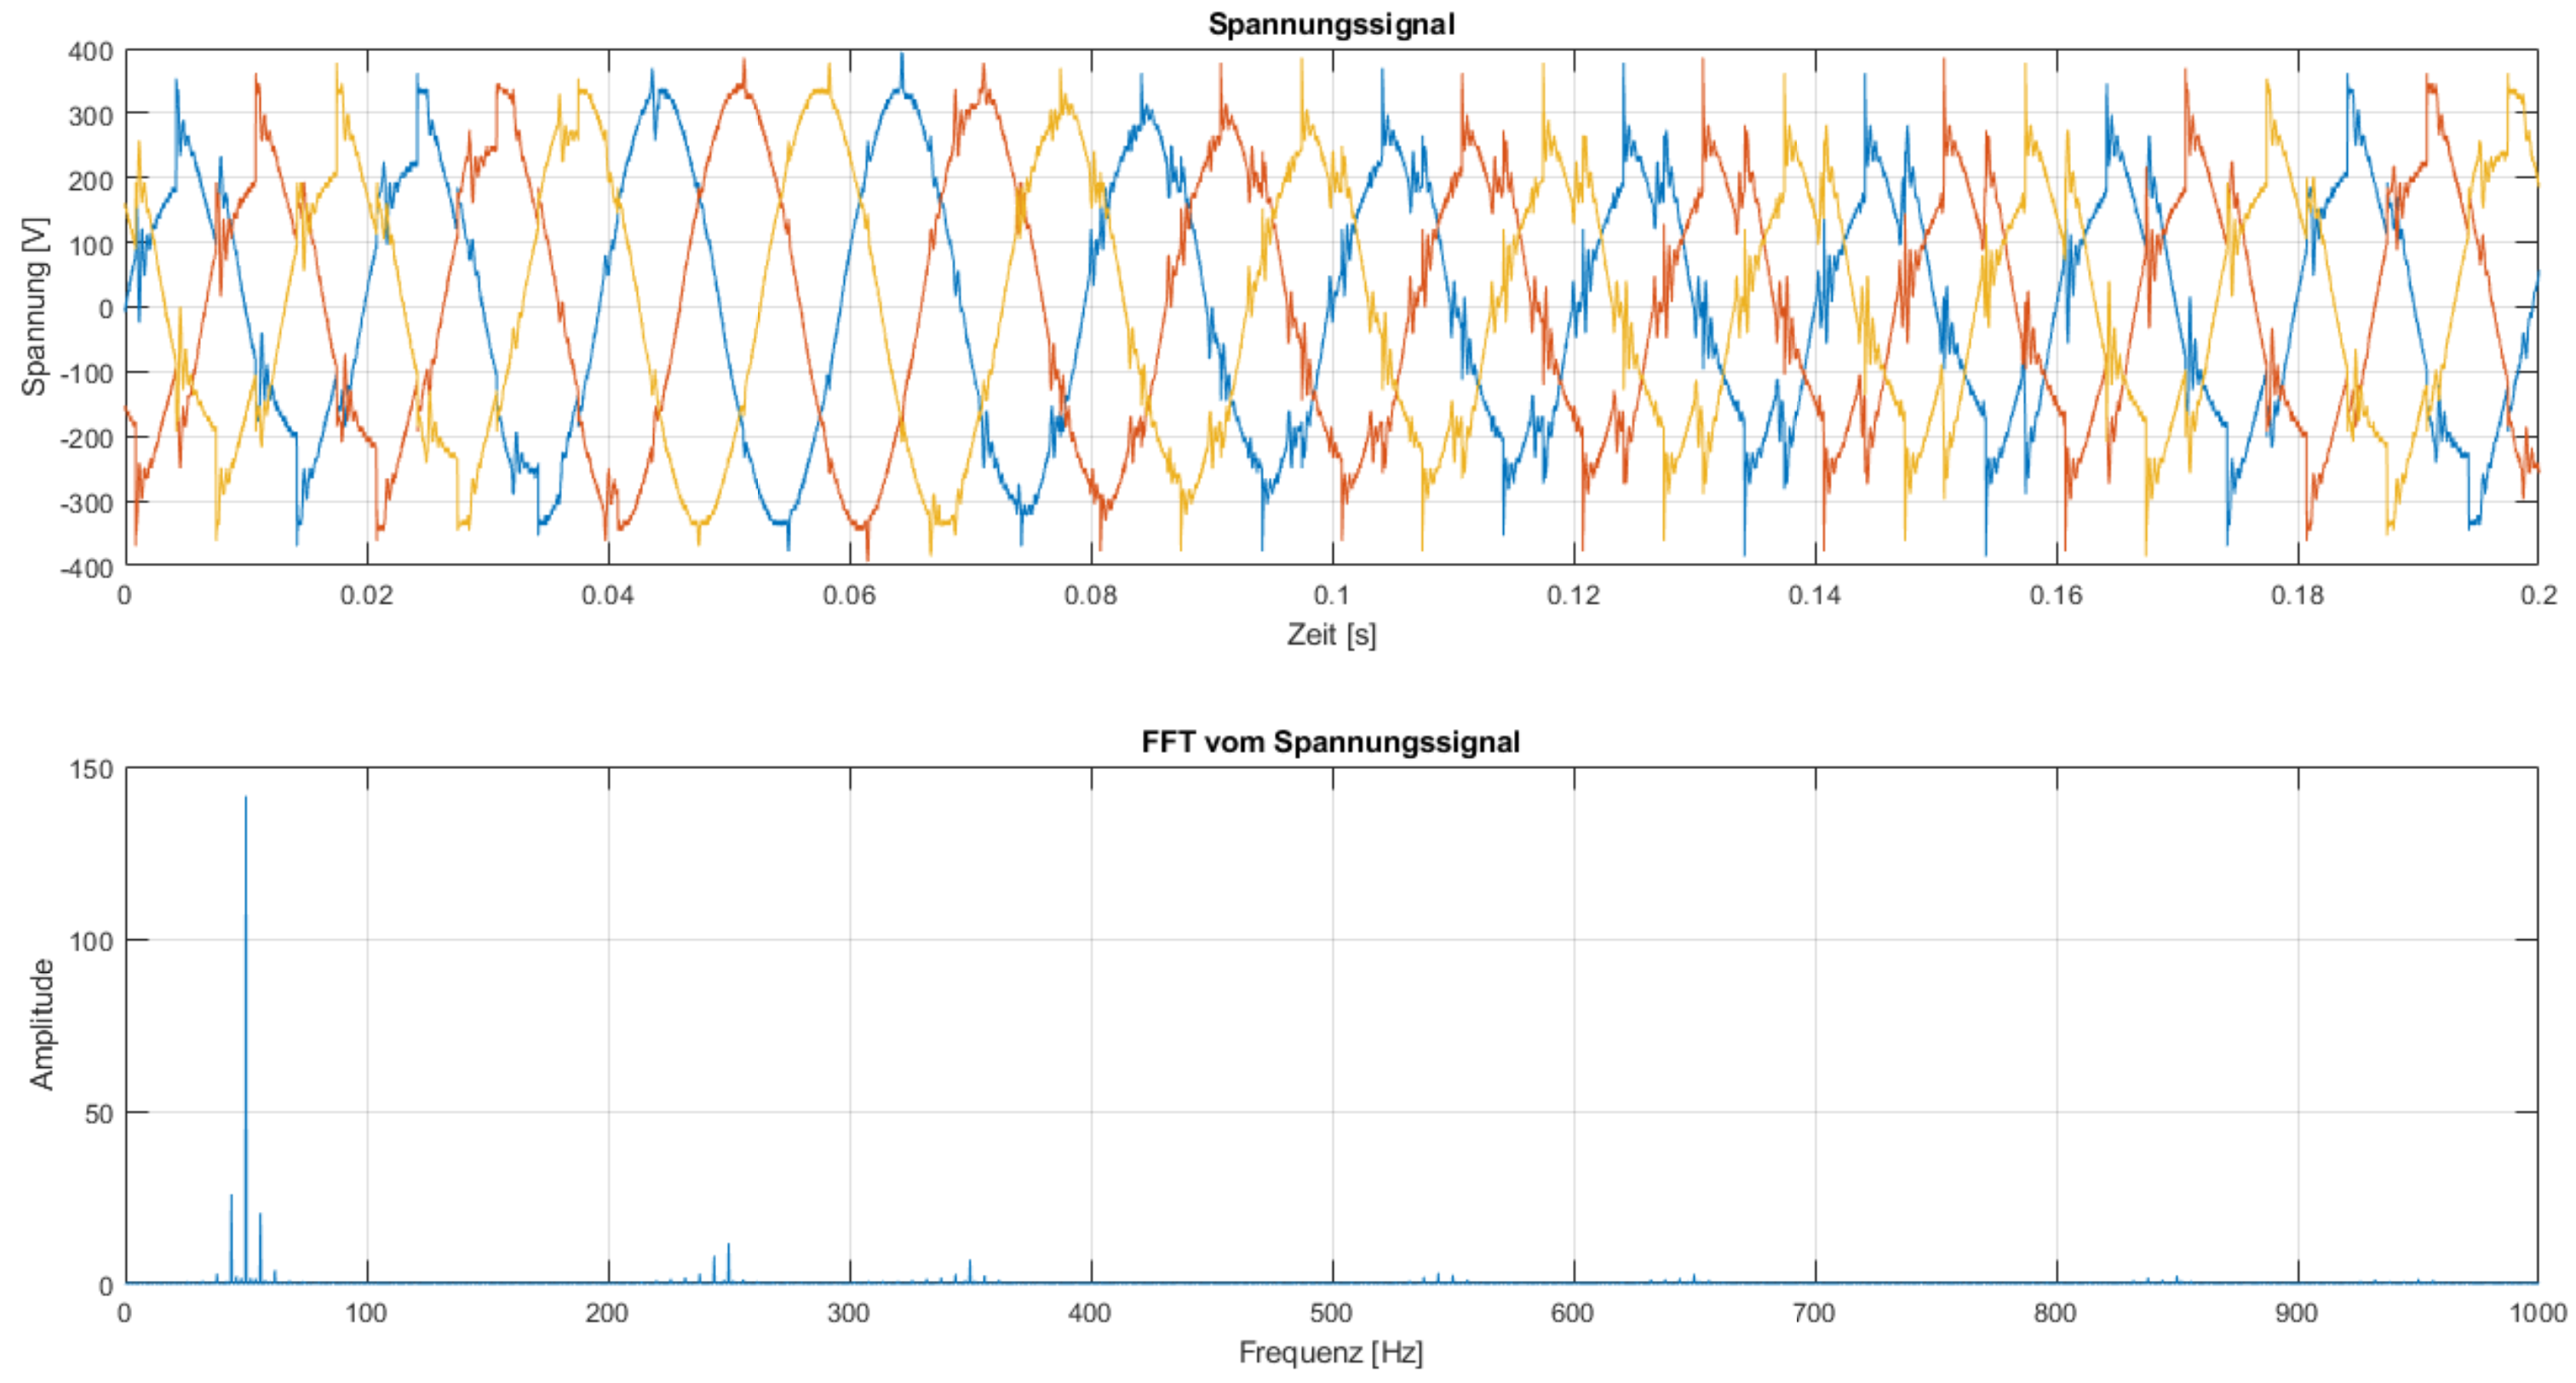
\includegraphics[width=\textwidth]{Messung_ASM_Phas_90grad.png}	
	\caption{Messung mit Phasenanschnitt 90\textdegree}\label{fig:Mess_ASM_Phas90}
\end{figure}

\begin{table}[ht!]
	\centering
	\begin{tabular}{|l|l|l|}
		\hline
		Frequenz {[}Hz{]} & Amplitude {[}V{]} & Verhältnis zur Grundschwingung \\ \hline
		44                & 25.896            & 18.31\%                        \\ \hline
		50                & 141.3976          & 100\%                          \\ \hline
		56                & 20.4508           & 14.46\%                        \\ \hline
		244               & 7.9778            & 5.64\%                         \\ \hline
		250               & 11.6537           & 8.24\%                         \\ \hline
		256               & 1.1655            & 0.82\%                         \\ \hline
		344               & 2.7272            & 1.93\%                         \\ \hline
		350               & 6.8988            & 4.88\%                         \\ \hline
		356               & 2.3509            & 1.66\%                         \\ \hline
	\end{tabular}
\caption{Amplitudenwerte bei der Frequenzen bei Phasenanschnitt 90\textdegree}\label{tab:Mess_Spannung_ASM_Phas90}
\end{table}

Anders als beim Phasenanschnitt mit 60\textdegree, beginnt der Asynchronmotor bei einem Winkel von 90\textdegree \hspace{0.02cm} zu schwingen. Dieses Schwingen ist in der Abbildung \ref{fig:Mess_ASM_Phas90} beim Spannungsverlauf ersichtlich. Wird das FFT betrachtet, sind sub- und zwischenharmonische, sowie harmonische Oberwellen erkennbar. Die Amplitudenwerte und das Verhältnis zur Grundschwingung ist für die 1., 5. und 7. Harmonischen, sowie deren Seitenbänder in der Tabelle \ref{tab:Mess_Spannung_ASM_Phas90} aufgelistet. Betrachtet man die Verhältnisse der harmonischen Oberwellen, sind die deutlich über den Werten der vorgeschriebenen Normen \ref{sec:Spannungsnormen}. Somit kann der Asynchronmotor nicht mit diesem Verfahren betrieben werden.  


\newpage
\subsubsection*{Sanftes Auf- und Absteuern}

Die Abbildung \ref{fig:Mess_ASM_Sanft_langsam} zeigt ein sanftes Auf- und Absteuern der Spannung.

\begin{figure}[ht!]
	\centering
	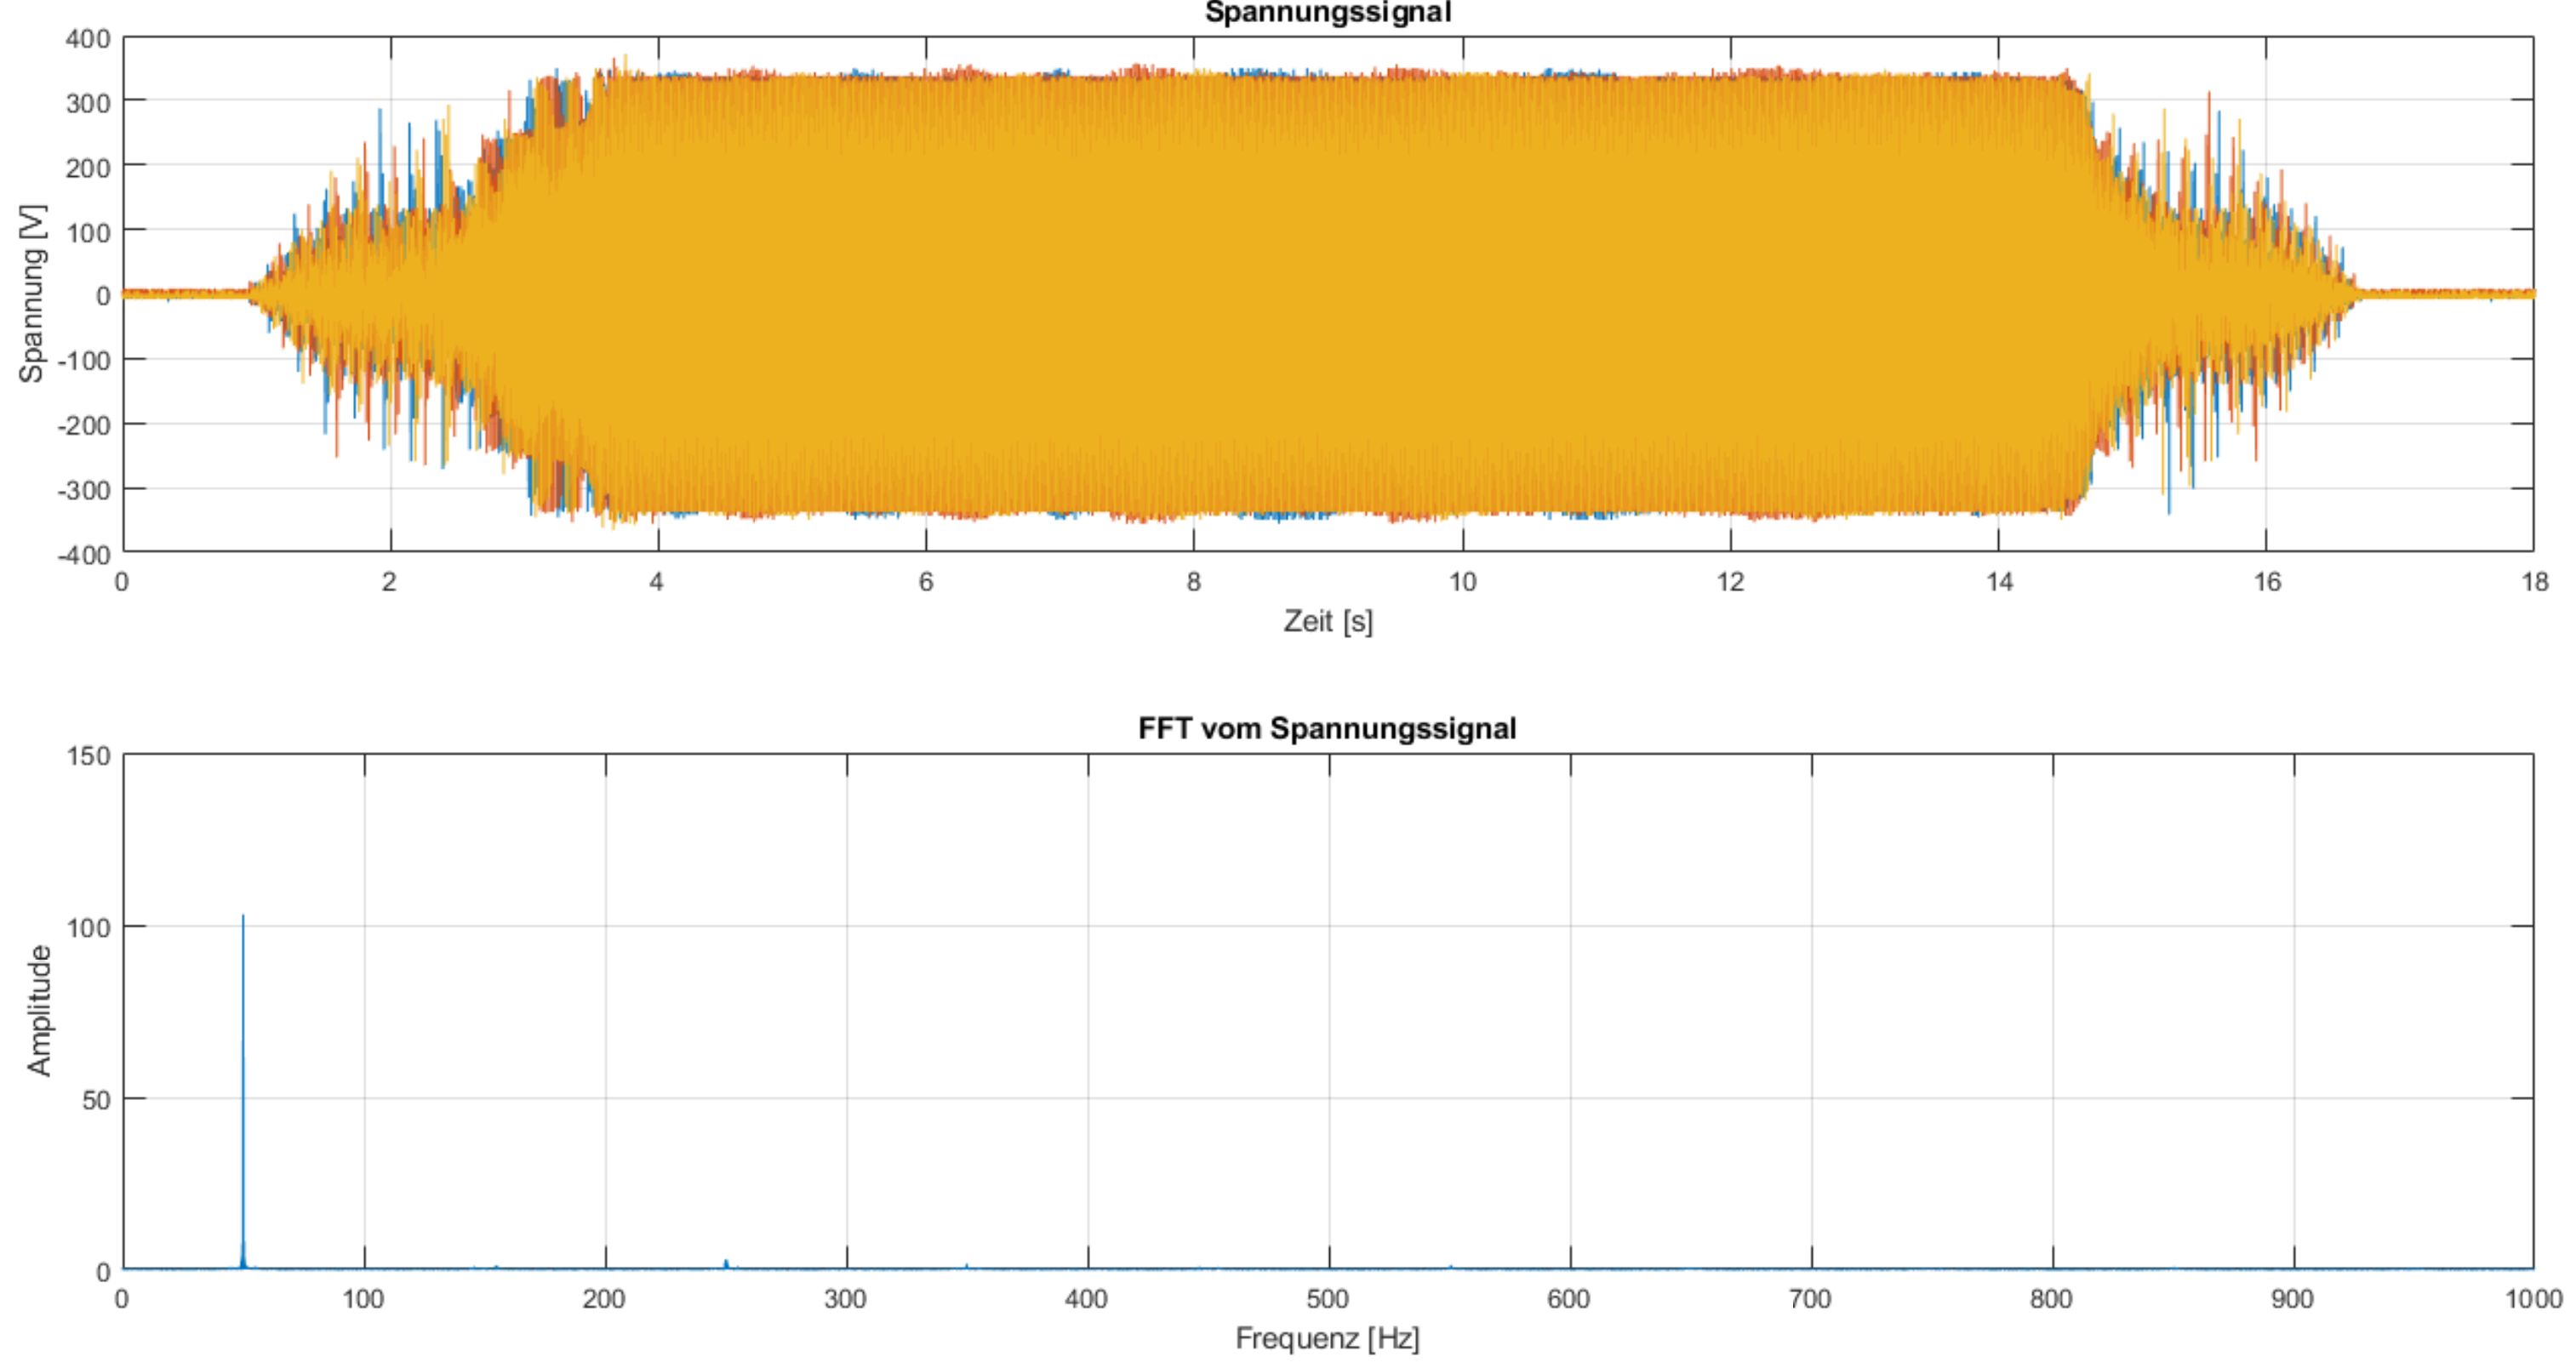
\includegraphics[width=\textwidth]{Messung_ASM_Sanft_langsam.png}	
	\caption{Messung mit sanftem Auf- und Absteuern}\label{fig:Mess_ASM_Sanft_langsam}
\end{figure}


\begin{table}[ht!]
	\centering
	\begin{tabular}{|l|l|l|}
		\hline
		Frequenz {[}Hz{]} & Amplitude {[}V{]} & Verhältnis zur Grundschwingung \\ \hline
		49.85             & 17.3653           & 16.85\%                        \\ \hline
		49.95             & 70.316            & 68.23\%                        \\ \hline
		50                & 103.0639          & 100\%                          \\ \hline
		50.05             & 40.167            & 38.97\%                        \\ \hline
		50.1              & 20.209            & 19.61\%                        \\ \hline
		249.95            & 2.607             & 2.53\%                         \\ \hline
		250               & 1.689             & 1.64\%                         \\ \hline
		250.05            & 2.5084            & 2.43\%                         \\ \hline
	\end{tabular}
\caption{Amplitudenwerte bei der Frequenzen bei sanftem Auf- und Absteuern}\label{tab:Mess_Spannung_ASM_AufAb_sanft}
\end{table}


Bei diesem Steuerungsverfahren sind die harmonischen Schwingungen mit den dazu gehörigen Seitenbänder nur noch minimal erkennbar. Die Resultate der Amplitudenwerte und das Verhältnis zur Grundschwingung befinden sich in der Tabelle \ref{tab:Mess_Spannung_ASM_AufAb_sanft}. Die meisten zwischenharmonischen Schwingungen treten um bei der Grundfrequenz von \SI{50}{Hz} auf. Es ist eine Ähnlichkeit zum Verfahren mit dem Widerstand ersichtlich. Vergleicht man die Werte der harmonischen Schwingungen mit den Normen \ref{sec:Spannungsnormen}, befinden diese sich unter den maximalen Grenzwerten. 



\newpage
\subsection{Sparvariante}
Wie im Kapitel \ref{Spar-Ansteuerung} beschrieben, werden bei der Sparvariante nur ein oder zwei Thyristoren angesteuert. Die Spannungs- und Stromsignale müssen dabei etwa die gleiche Form besitzen wie bei der dreiphasigen Ansteuerung. Da dies bei der Ansteuerung mit einem Thyristor nicht der Fall ist, sind die Messresultate bei diesem Verfahren nicht aufgeführt. Für die Sparvarianten wurden die Verfahren des sanften und harten Auf- und Absteuern betrachtet, da hauptsächlich diese von Interesse sind. Bei den Messungen ist ersichtlich, dass die harmonischen Oberwellen der Spannung des Asynchronmotors die Vorgaben der Normen nicht erfüllt. Das gleiche Verhalten wurde bei der ohmschen Last mit harter Ansteuerung bemerkt. Daher wird nur noch das sanfte Hoch- und Runterfahren beim Widerstand analysiert. Alle anderen Messungen, die nicht den Normen entsprechen, sind im Anhang im Kapitel \ref{sec:Sparvariante_2Thyristoren} ersichtlich. Die Abbildungen \ref{fig:Mess_2Thyristoren_Widerstand_AufAbFahren_langsam_stroeme} und \ref{fig:Mess_2Thyristoren_Widerstand_AufAbFahren_langsam} sind so aufgebaut, dass zuerst das Spannungs- oder Stromsignal ersichtlich ist. Anschliessend werden die FFT der drei Phasen berechnet und dargestellt. Da es sich um eine unsymmetrische Belastung handelt, wurden alle Phasen separat mit den Normen \ref{sec:Normen} verglichen.

\subsubsection{Strommessung Sparvariante mit einem Widerstand und zwei Thyristoren}

In der Abbildung \ref{fig:Mess_2Thyristoren_Widerstand_AufAbFahren_langsam_stroeme} erkennt man ein sanftes Hoch- und Herunterfahren des Stromes, gemessen durch den Widerstand.

\begin{figure}[ht]
	\centering
	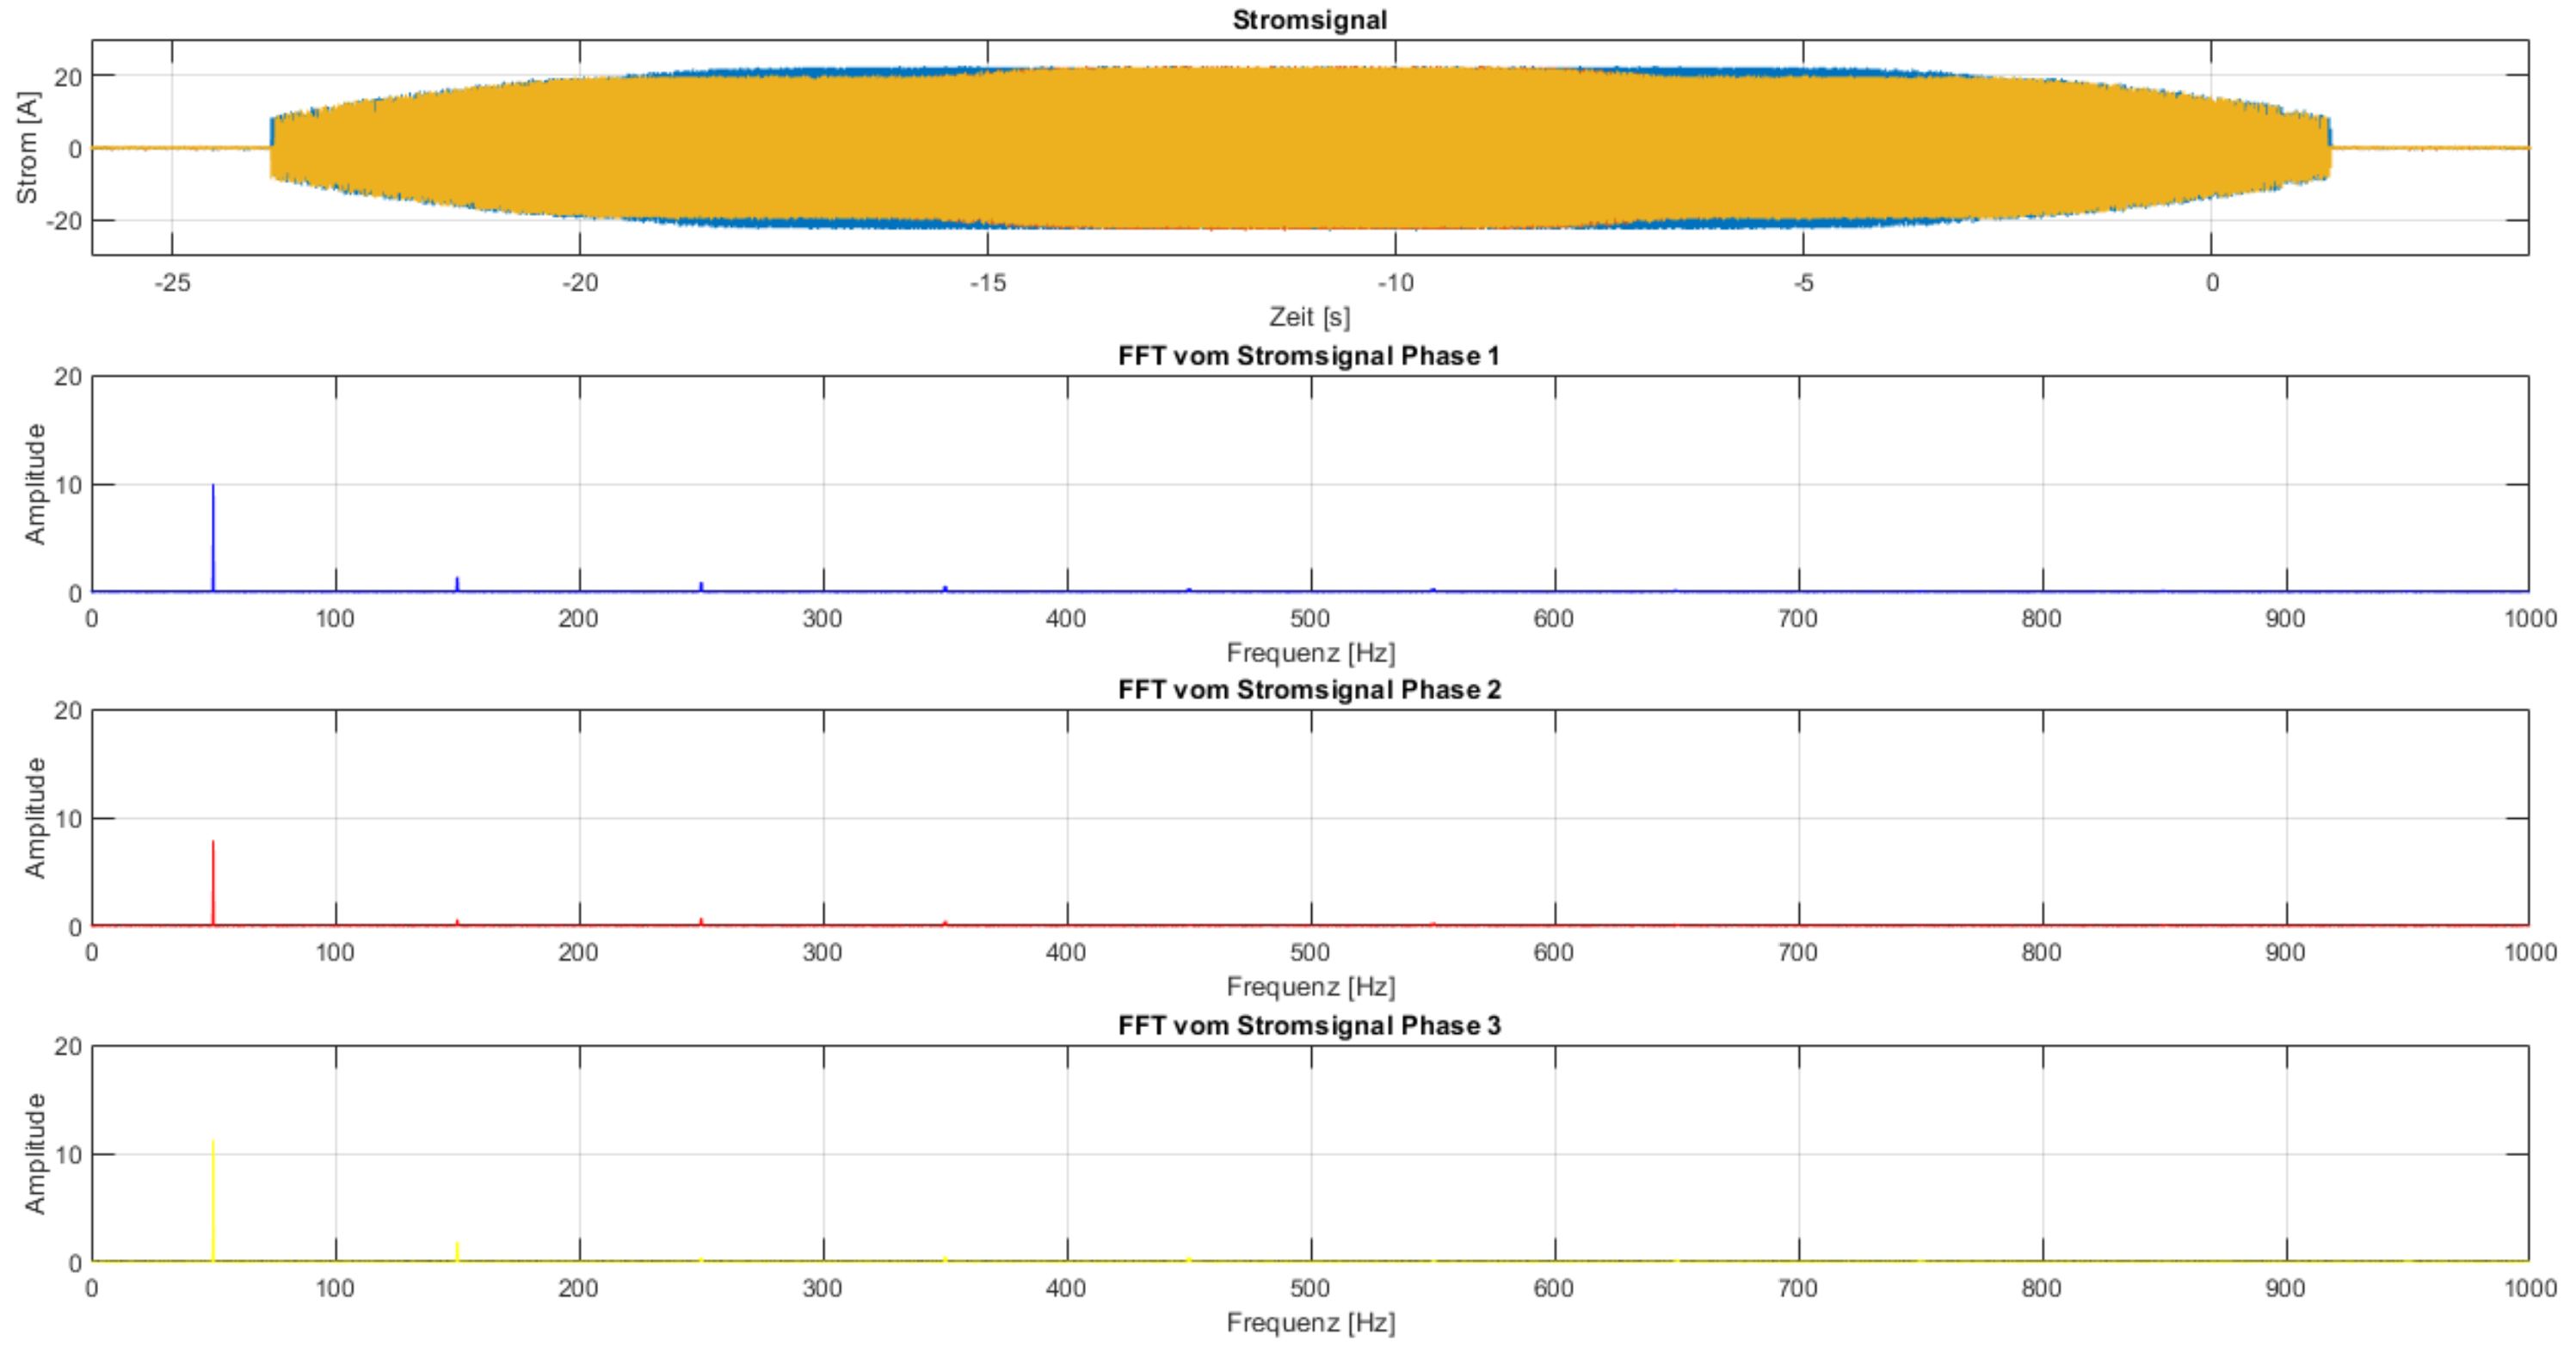
\includegraphics[width=\textwidth]{Messung_Widerstand_2Thyristoren_Stroeme.png}	
	\caption{Strommessung mit dem sanften Auf- und Absteuern und zwei Thyristoren}\label{fig:Mess_2Thyristoren_Widerstand_AufAbFahren_langsam_stroeme}	
\end{figure}

\begin{table}[ht]
	\centering
	\begin{tabular}{|l|l|l|l|}
		\hline
		Frequenz {[}Hz{]} & Amplitude Phase 1 {[}A{]}                                                           & Amplitude Phase 2 {[}A{]}                                                           & Amplitude Phase 3 {[}A{]}                                                           \\ \hline
		49.9              & 4.887                                                                               & 3.749                                                                               & 2.354                                                                               \\ \hline
		49.95             & 9.018                                                                               & 7.485                                                                               & 9.618                                                                               \\ \hline
		50                & 9.951                                                                               & 7.881                                                                               & 11.225                                                                              \\ \hline
		50.05             & 5.193                                                                               & 4.31                                                                                & 3.031                                                                               \\ \hline
		50.1              & 3.057                                                                               & 1.522                                                                               & 1.809                                                                               \\ \hline
		149.93            & 1.381                                                                               & 0.525                                                                               & 1.838                                                                               \\ \hline
		150               & 0.899                                                                               & 0.552                                                                               & 1.103                                                                               \\ \hline
		150.2             & 1.386                                                                               & 0.544                                                                               & 1.829                                                                               \\ \hline
		250		          & 0.372                                                                               & 0.273                                                                               & 0.291                                                                               \\ \hline \hline
		Frequenz {[}Hz{]} & \begin{tabular}[c]{@{}l@{}}Verhältnis zur \\ Grundschwingung\\ Phase 1\end{tabular} & \begin{tabular}[c]{@{}l@{}}Verhältnis zur \\ Grundschwingung\\ Phase 2\end{tabular} & \begin{tabular}[c]{@{}l@{}}Verhältnis zur \\ Grundschwingung\\ Phase 3\end{tabular} \\ \hline
		49.9              & 49.11\%                                                                             & 47.57\%                                                                             & 20.97\%                                                                             \\ \hline
		49.95             & 90.62\%                                                                             & 94.98\%                                                                             & 85.68\%                                                                             \\ \hline
		50                & 100\%                                                                               & 100\%                                                                               & 100\%                                                                               \\ \hline
		50.05             & 52.19\%                                                                             & 54.69\%                                                                             & 27\%                                                                                \\ \hline
		50.1              & 30.72\%                                                                             & 19.32\%                                                                             & 16.12\%                                                                             \\ \hline
		149.95            & 13.88\%                                                                             & 6.66\%                                                                              & 16.37\%                                                                             \\ \hline
		150               & 9.03\%                                                                              & 7\%                                                                                 & 9.83\%                                                                              \\ \hline
		150.05            & 13.93\%                                                                             & 6.9\%                                                                               & 16.29\%                                                                             \\ \hline
		250		          & 3.74\%                                                                             & 3.46\%                                                                               & 2.59\%                                                                             \\ \hline
	\end{tabular}
	\caption{Amplitudenwerte bei der Strommessung mit zwei Thyristoren bei sanftem Auf- und Absteuern}\label{tab:Mess_2Thyristoren_Spannung_Widerstand_AufAb_sanft_stroeme}
\end{table}

Damit die Oberschwingungsströme mit den  Grenzwerten der Normen \ref{sec:Stromnormen} verglichen werden können, wurde der Effektivwert des Stromes auf \SI{16}{A} hochgerechnet. Betrachtet man die verschiedenen FFTs der Phasen sind unterschiedliche Peak-Werte zu erkennen. Dies kommt zustande, da es sich um eine unsymmetrische Belastung handelt und die Phase 3 als Rückleiter fungiert. In der Tabelle \ref{tab:Mess_2Thyristoren_Spannung_Widerstand_AufAb_sanft_stroeme} werden die Werte der Amplituden bei verschiedenen Frequenzen und das Verhältnis zur Grundschwingung aufgelistet. Vergleicht man die Werte der 3. und 5. Harmonischen mit den Normen \ref{sec:Stromnormen}, so halten sie die Grenzwerte bei allen drei Phasen ein. Die anderen harmonischen Schwingungen, die nicht in der Tabelle sind, halten die Normen ebenfalls ein.

\newpage
\subsubsection{Spannungsmessung Sparvariante mit einem Widerstand und zwei Thyristoren}

Die Abbildung \ref{fig:Mess_2Thyristoren_Widerstand_AufAbFahren_langsam} zeigt das Spannungssignal über dem Widerstand. 

\begin{figure}[ht!]
	\centering
	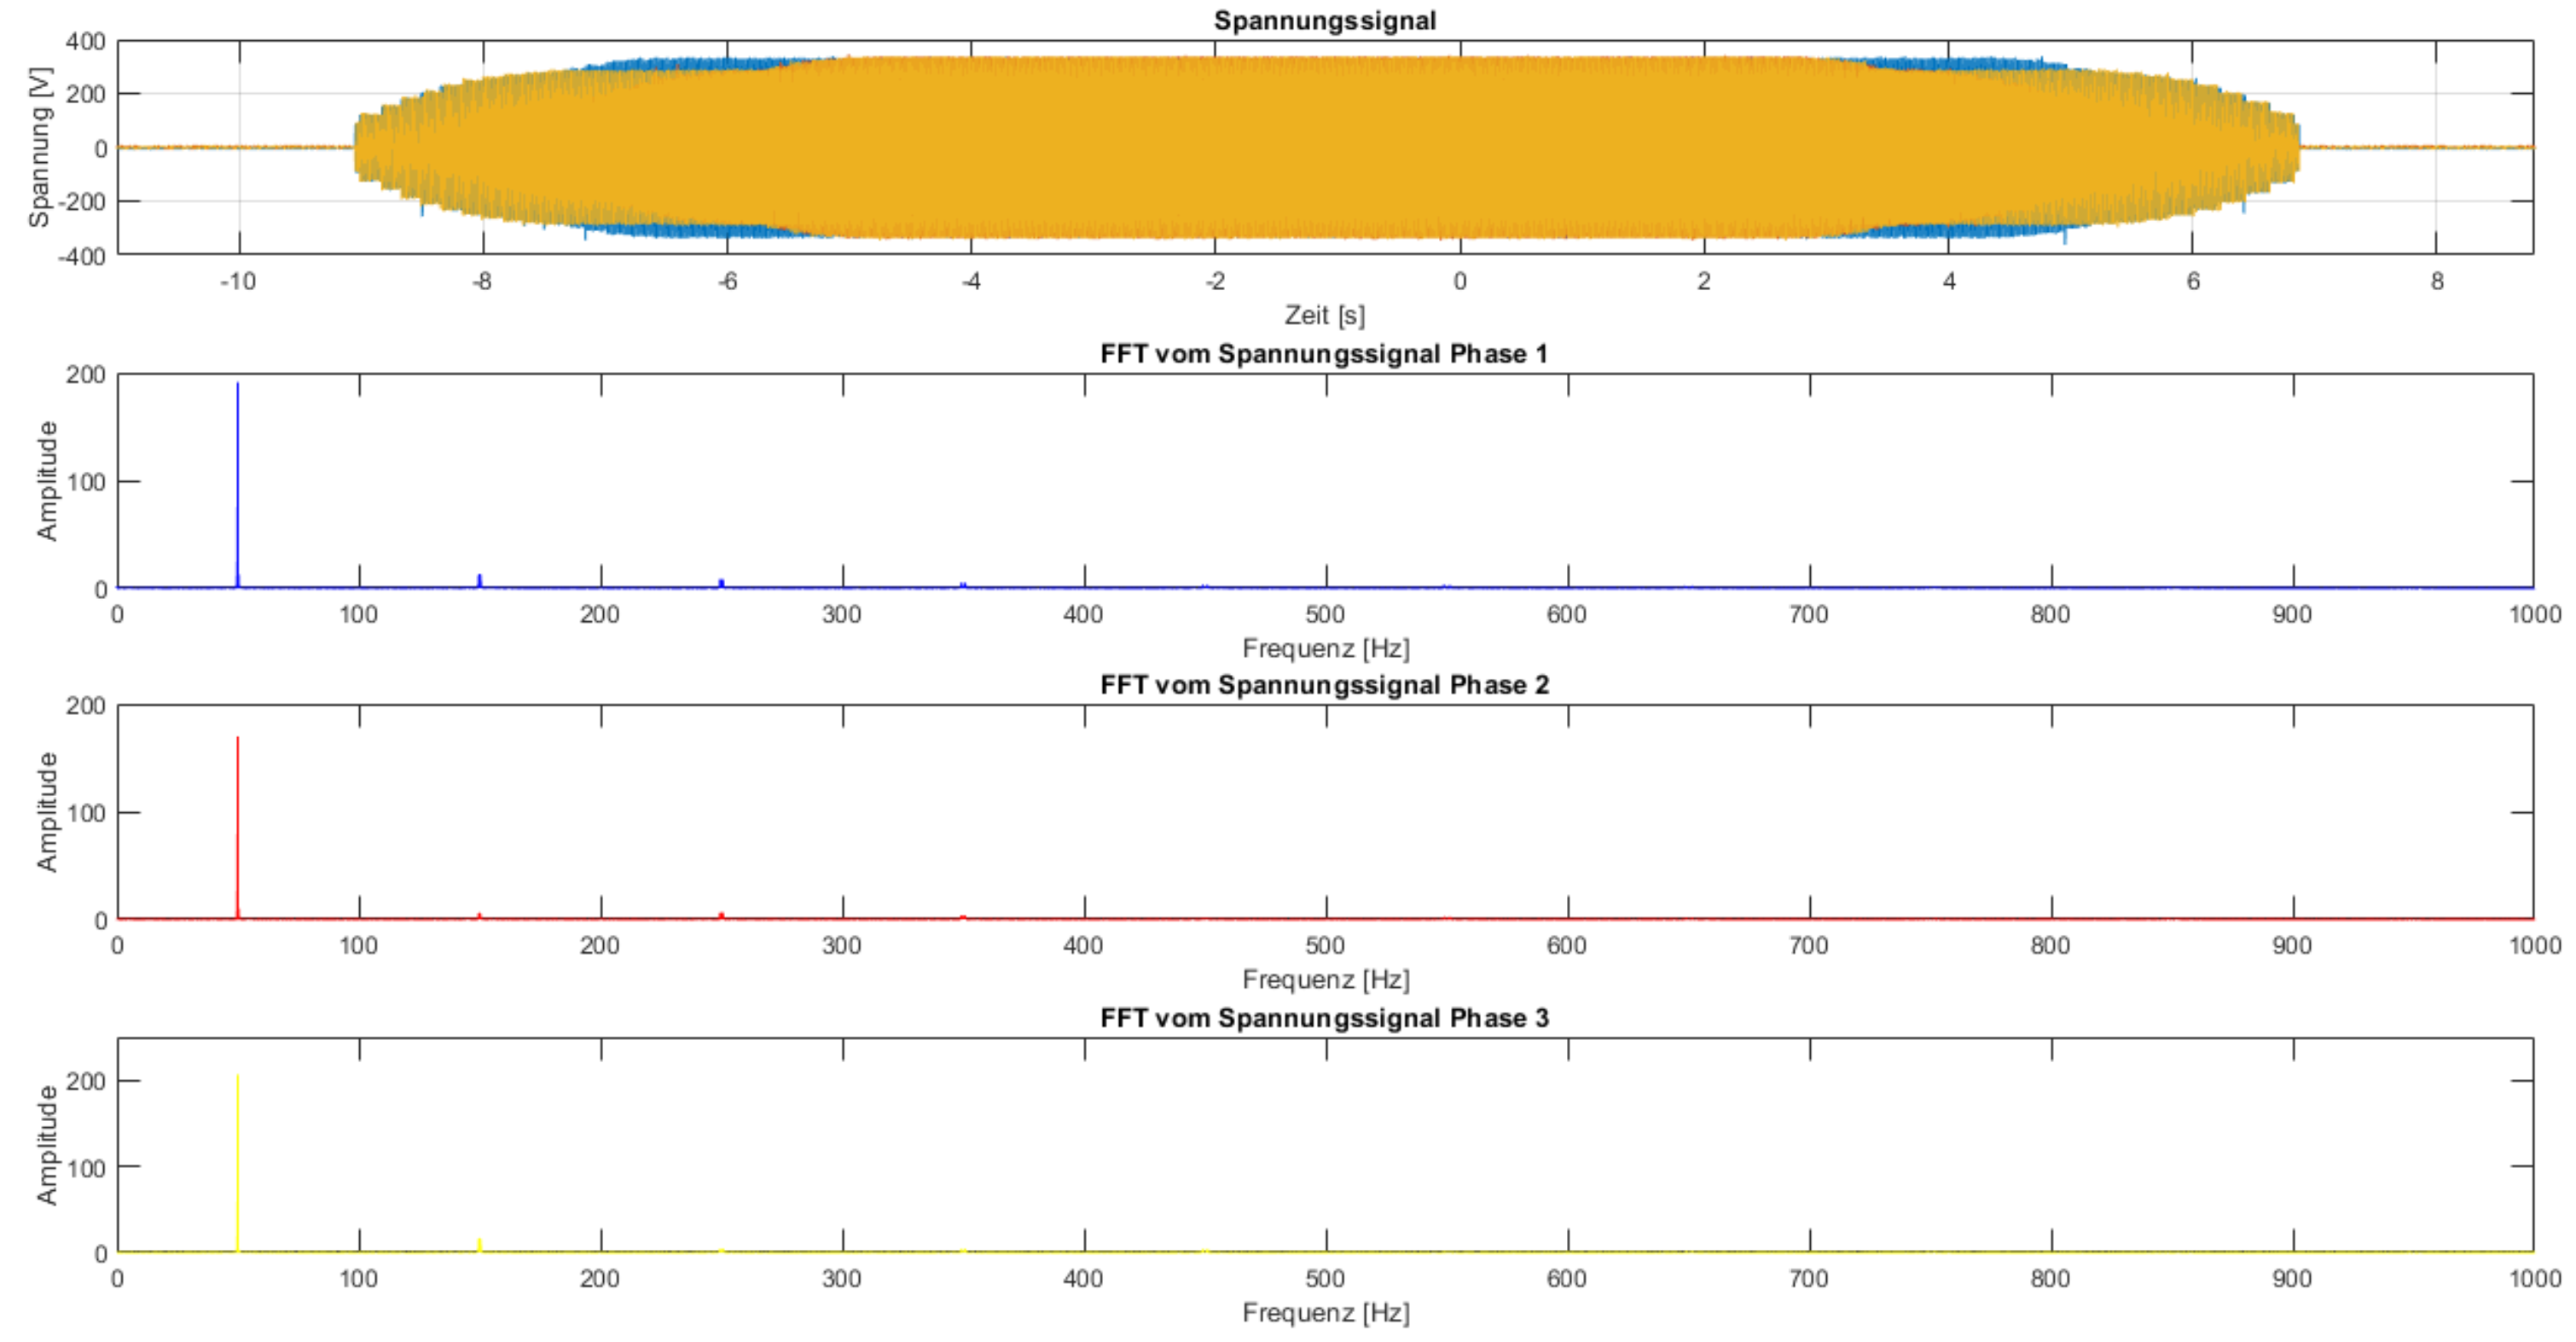
\includegraphics[width=\textwidth]{Mess_2Thyristoren_Widerstand_AufAbFahren_langsam.png}	
	\caption{Messung mit dem sanften Auf- und Absteuern und zwei Thyristoren}\label{fig:Mess_2Thyristoren_Widerstand_AufAbFahren_langsam}	
\end{figure}

Die Spannungsverläufe auf der Abbildung \ref{fig:Mess_2Thyristoren_Widerstand_AufAbFahren_langsam} sehen visuell ähnlich aus wie das sanfte Auf- und Absteuern mit drei Thyristoren, ersichtlich in der Abbildung \ref{fig:Mess_Sanft_langsam}.  Der einziger Unterschied ist, dass beim Hoch- und Runterfahren die drei Phasen nicht alle gleich hoch sind. Dies resultiert in einem FFT mit unterschiedlichen Amplitudenhöhen für die verschiedenen Phasen. Die Werte des FFTs sind in der Tabelle \ref{tab:Mess_2Thyristoren_Spannung_ASM_AufAb_sanft} aufgelistet. \\\\

\begin{table}[ht!]
	\centering
	\begin{tabular}{|l|l|l|l|}
		\hline
		Frequenz {[}Hz{]} & Amplitude Phase 1 {[}V{]}                                                           & Amplitude Phase 2 {[}V{]}                                                           & Amplitude Phase 3 {[}V{]}                                                           \\ \hline
		49.9              & 38.5998                                                                             & 19.6499                                                                             & 34.7131                                                                             \\ \hline
		49.95             & 77.5993                                                                             & 82.1127                                                                             & 60.2946                                                                             \\ \hline
		50                & 191.1857                                                                            & 169.7545                                                                            & 206.7036                                                                            \\ \hline
		50.05             & 125.8716                                                                            & 123.6057                                                                            & 126.0935                                                                            \\ \hline
		50.1              & 42.6127                                                                             & 17.4015                                                                             & 26.3464                                                                             \\ \hline
		149.8             & 12.7189                                                                             & 3.9393                                                                              & 16.14                                                                               \\ \hline
		150               & 2.6765                                                                              & 4.3294                                                                              & 5.5055                                                                              \\ \hline
		150.2             & 9.6611                                                                              & 5.9313                                                                              & 13.152                                                                              \\ \hline
		250             & 2.05                                                                              & 0.641                                                                              & 2.334                                                                              \\ \hline \hline
		Frequenz {[}Hz{]} & \begin{tabular}[c]{@{}l@{}}Verhältnis zur \\ Grundschwingung\\ Phase 1\end{tabular} & \begin{tabular}[c]{@{}l@{}}Verhältnis zur \\ Grundschwingung\\ Phase 2\end{tabular} & \begin{tabular}[c]{@{}l@{}}Verhältnis zur \\ Grundschwingung\\ Phase 3\end{tabular} \\ \hline
		49.9              & 20.19\%                                                                             & 11.58\%                                                                             & 16.79\%                                                                             \\ \hline
		49.95             & 40.59\%                                                                             & 48.37\%                                                                             & 29.17\%                                                                             \\ \hline
		50                & 100\%                                                                               & 100\%                                                                               & 100\%                                                                               \\ \hline
		50.05             & 65.84\%                                                                             & 72.81\%                                                                             & 61\%                                                                                \\ \hline
		50.1              & 22.29\%                                                                             & 10.25\%                                                                             & 12.75\%                                                                             \\ \hline
		149.8             & 6.65\%                                                                              & 2.32\%                                                                              & 7.81\%                                                                              \\ \hline
		150               & 1.4\%                                                                               & 2.55\%                                                                              & 2.66\%                                                                              \\ \hline
		150.2             & 5.05\%                                                                              & 3.49\%                                                                              & 6.36\%                                                                              \\ \hline
		250             & 1.07\%                                                                              & 0.38\%                                                                              & 1.13\%                                                                              \\ \hline
		
	\end{tabular}
\caption{Amplitudenwerte bei der Frequenzen mit zwei Thyristoren bei sanftem Auf- und Absteuern}\label{tab:Mess_2Thyristoren_Spannung_Widerstand_AufAb_sanft}
\end{table}

Das Spannungssignal, welches mit nur zwei Thyristoren angesteuert wurde, hat eine visuelle Ähnlichkeit mit dem sanften Auf- und Absteuern der drei Thyristoren \ref{fig:Mess_Sanft_langsam}. Der einzige Unterschied entsteht beim Hoch- und Runterfahren. Die drei Phasen erreichen wegen der unsymmetrischen Belastung nicht die gleiche Höhe. Dies ist bei den FFT ebenfalls ersichtlich. Es sind unterschiedliche Amplitudenhöhen aufgezeigt. Die Werte der FFTs sind in der Tabelle \ref{tab:Mess_2Thyristoren_Spannung_ASM_AufAb_sanft} aufgelistet. Vergleicht man wiederum die Werte der harmonischen Schwingungen mit den Grenzwerten der Normen, erfüllen sie jedoch den einzuhaltenden Bereich.


\newpage
\subsection{Leistungsfaktor}
Um den Leistungsfaktor für den Phasenanschnitt berechnen zu können, werden die Formeln im Kapitel \ref{sec:Leistungsfaktor} verwendet. Jedoch funktionieren diese Formeln bei der Kombination der verschiedenen Verfahren oder dem Hochfahren durch den Phasenanschnitt nicht. Mit folgender Formel kann der Leistungsfaktor ebenfalls berechnet werden:
\begin{equation}
\lambda = \frac{P}{S}
\end{equation}
Um die Wirkleistung zu erhalten, können die Strom- und Spannungswerte multipliziert werden:
\begin{equation}
P = u(t) \cdot i(t)
\end{equation}
Für die Scheinleistung müssen die Effektivwerte der Spannung und des Stromes multipliziert werden:
\begin{equation}
S = U_{rms} \cdot I_{rms}
\end{equation}
Wobei der Effektivwert des Stromes und der Spannung über die gesamte Zeitdauer berechnet wurde. Der Matlabcode dieser Berechnungen befindet sich im Anhang im Kapitel \ref{sec:Leistungsfaktor_Messungen}. 

Die Resultate der Leistungsfaktorberechnungen sind in der Tabelle \ref{tab:Leistungsfaktor_ASM_Widerstand} aufgeführt.

\begin{table}[ht!]
	\centering
	\begin{tabular}{|l|l|}
		\hline
		Ansteuerungsart ASM                                   		& Leistungsfaktor \\ \hline 
		Sanftes Auf- und Absteuern                          		& 0.2947          \\ \hline
		Sanftes Auf- und Absteuern mit 150$\Omega$ Vorwiderstand 	& 0.3493          \\ \hline
		Phasenanschnitt 90\textdegree                               & 0.4879          \\ \hline
		Phasenanschnitt 60\textdegree                               & 0.4155          \\ \hline \hline
		Ansteuerungsart Widerstand                            		& Leistungsfaktor \\ \hline 
		Sanftes Auf- und Absteuern                          		& 0.9987          \\ \hline
		Hartes Auf- und Absteuern                                   & 0.9988          \\ \hline
		Phasenanschnitt 90\textdegree                         		& 0.9953          \\ \hline
		Phasenanschnitt 60\textdegree                         		& 0.999           \\ \hline
	\end{tabular}
\caption{Leistungsfaktor mit verschiedene Ansteuerungsverfahren bei der ASM und dem Widerstand}\label{tab:Leistungsfaktor_ASM_Widerstand}
\end{table}
Bei der ASM im Leerlauf gilt, je näher der Leistungsfaktor bei 0 ist desto besser. Da der Leistungsfaktor das Verhältnis von Wirk- zu Scheinleistung ist und sich die Maschine im Leerlauf befindet, wird die Wirkleistung nur für die Ummagnetisierungs- und Eisenverluste benötigt. Wenn der Leistungsfaktor höher ist, heisst dies, dass mehr Verlustleistung entsteht. Um dies zu beweisen wurde ein Vorwiderstand mit \SI{150}{\Omega} in den Stromkreis geschaltet. Dabei konnte festgestellt werden, dass sich wie erwartet mit dem Vorwiderstand der Leistungsfaktor erhöht, da zusätzlich Wirkleistung im Widerstand verheizt wird. Wenn die Leistungsfaktoren der verschiedenen Ansteuerungsarten miteinander verglichen werden, kann klar gesagt werden, dass sich das sanfte Auf- und  Absteuern am besten eignet für die ASM.

Bei Ohmschen Lasten gilt jedoch, je näher der Leistungsfaktor bei 1 ist, desto besser. Bei den Messungen mit den verschiedenen Ansteuerungsarten wurde festgestellt, dass der Leistungsfaktor beim Phasenanschnitt mit einem Winkel von 60\textdegree \hspace{0.02cm} am höchsten ist. Jedoch verbieten die Normen den Gebrauch des Phasenanschnittes mit den Winkeln von 90\textdegree \hspace{0.02cm} wegen den erhöhten Werten der Amplituden. Deshalb macht es Sinn, nur das sanfte und harte Auf- und Abfahren zu vergleichen. Bei diesen zwei Ansteuerungsverfahren hat das harte Auf- und Absteuern einen höheren Leistungsfaktor. Jedoch ist der Unterschied von 0.0001 sehr klein und kann praktisch vernachlässigt werden.
 



%\subsubsection{Schwingungspaketsteuerung mit Last in Stern}
%Für die Messung mit der Schwingungspaketsteuerung wurde eine Einschaltzeit von 0.5 Sekunden und eine Ausschaltzeit von 0.2 Sekunden gewählt. Die Ausschaltzeit darf nicht kürzer sein, da die Spannungsverstärkerschaltung und den Thyristorsteller eine Zeitverzögerung darstellen und so die Spannung nicht sofort ein- oder ausgeschaltet wird. Wenn die Ausschaltzeit kürzer ist, geht die Spannung zwischen den Paketen nicht auf \SI{0}{V}. 
%\begin{figure}[ht!]
%	\centering
%	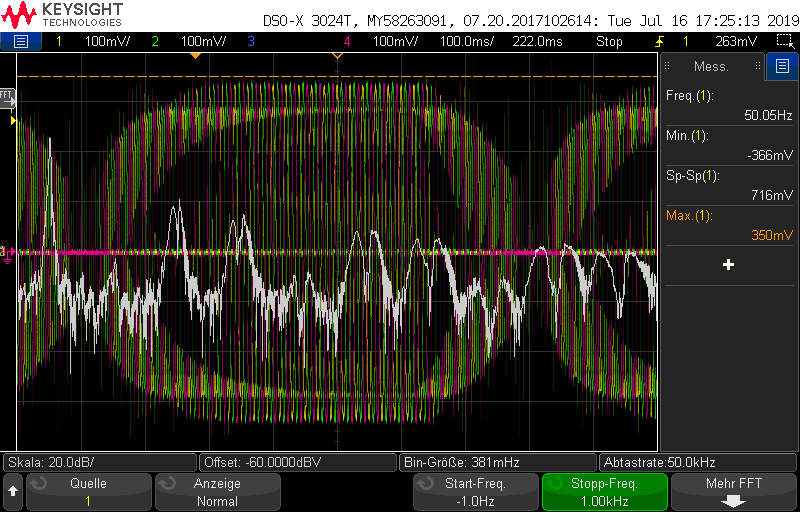
\includegraphics[width=0.7\textwidth]{Schwingungspaket_kurz.png}	
%	\caption{Das Spannungssignal aller Phasen bei Schwingungspaketsteuerung mit FFT}\label{fig:Mess_Schwing_kurz}
%\end{figure}
%
%Das FFT zeigt entgegen den Erwartungen aus der Theorie fast keine Subharmonische auf. Dafür sind Harmonische und Zwischehamrnische sehr ausgeprägt. Sehr gut zu sehen ist die Grundfrequenz von \SI{50}{Hz}, der erste Peak von der linken Seite. Dies ist darauf zurückzuführen, dass nicht direkt ein- und ausgeschaltet wird und so einem Sanft-Anlass ähnelt. Dies dominiert gegenüber dem harten Ein- und Ausschalten, welches die Subharmonische hervorrufen würde.
%\newpage
%\subsection{Phasenanschnittsteuerung mit 2 Thyristoren mit Last in Stern}
%Für die Sparansteuerung wurde ein Winkel von 90\textdegree \hspace{0.02cm} gewählt. 
%
%\begin{figure}[ht!]
%	\centering
%	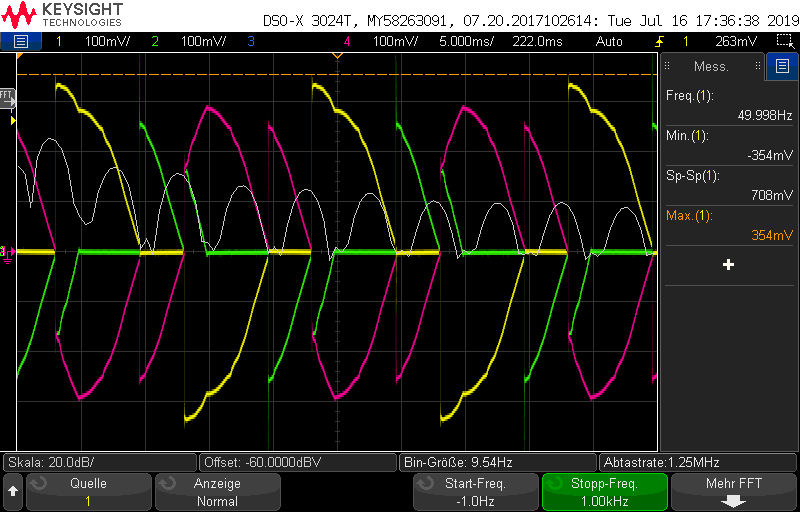
\includegraphics[width=0.7\textwidth]{2phas_90grad_kurz.png}	
%	\caption{Das Spannungssignal aller Phasen bei Schwingungspaketsteuerung mit FFT}\label{fig:Mess_2phas_kurz}
%\end{figure}
%
%
%\subsection{Phasenanschnittsteuerung mit 1 Thyristor mit Last in Stern}
%Für die Sparansteuerung wurde ein Winkel von 90\textdegree gewählt. 
%
%\begin{figure}[ht!]
%	\centering
%	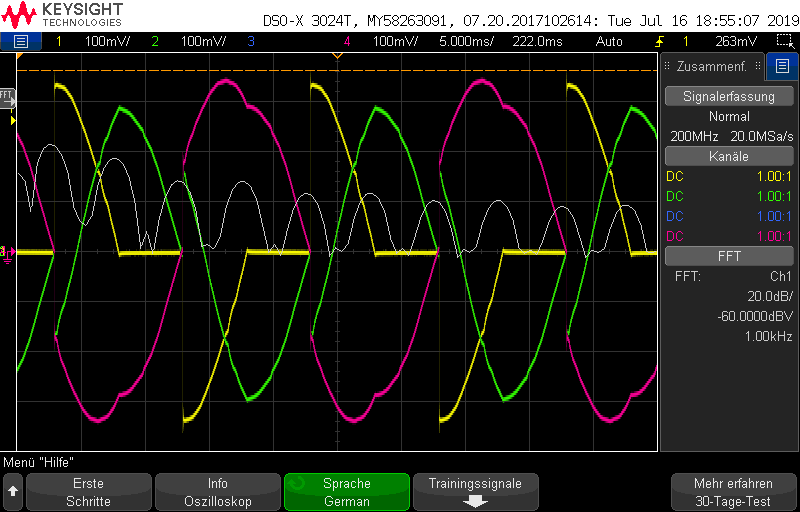
\includegraphics[width=0.7\textwidth]{1phas_90grad_kurz.png}	
%	\caption{Das Spannungssignal aller Phasen bei Schwingungspaketsteuerung mit FFT}\label{fig:Mess_1phas_kurz}
%\end{figure}




